\documentclass[table, 13pt, slidestop,compress,mathserif]{beamer}
%%==========================================================
\usepackage[english]{babel} % 如果去掉,中英文混合会有问题
\usepackage[UTF8, zhmap = true]{ctex} %增加中文处理
\usepackage{tikz} %绘图命令

\usepackage{framed, xcolor} 
\usepackage{tabularx, colortbl, booktabs, multirow, makecell, longtable}
\usepackage{animate}

\usepackage{soul} %for strikeout

\usepackage{amsmath, amsfonts, amssymb} %amssymb for varnothing symbol
\usepackage{blkarray} % support complicated matrix
%\usepackage[thicklines]{cancel} %公式中通过斜线删除部分内容
\usepackage[b]{esvect} %vector

\usepackage{caption, algorithm}
\usepackage[noend]{algpseudocode}

\usepackage{textpos}
\usepackage{adjustbox} %调整大小,例如缩放tikz绘图结果

\usepackage{pgfplots}
\usepackage{tikz, flowchart,times} % tikz绘图
\usepackage{smartdiagram}
\usetikzlibrary{decorations.pathreplacing}
\usetikzlibrary{decorations.markings}
\usetikzlibrary{calc, arrows, arrows.meta, shapes,snakes, shapes.geometric, positioning}
\usetikzlibrary{topaths}
\usetikzlibrary{mindmap, backgrounds}
\usetikzlibrary{shadings}
\usetikzlibrary{shadows}
\usetikzlibrary{graphs}
\usetikzlibrary{matrix}
\usetikzlibrary{patterns}

\usepackage{tkz-graph}
\usepackage{forest}
\forestset{
  default preamble={
    for tree={circle,draw}
  },
  gappy tree/.style={
    for tree={
      circle,
      draw,
      s sep'+=10pt,
      fit=band,
    },
  },
  missed/.style={draw=none, no edge}
}

\usepackage{environ}
\NewEnviron{tikzthm}[1]{
\begin{tikzpicture}
\node [newthemsty] (box){\BODY};
\node[newthemstytitle, right=10pt] at (box.north west) {\textbf{#1}};
\end{tikzpicture}
}

% 新建幻灯片每一小节开始的样式环境
\NewEnviron{sectionbox}[1]{
  \begin{center}
    \tikzstyle{mybox} = [draw=blue, fill=green!20, very thick,
    rectangle, rounded corners, inner sep=10pt, inner ysep=20pt]
    \tikzstyle{fancytitle} =[fill=blue, text=white, ellipse]
    
    \vspace{1.0cm}
    \begin{tikzpicture}[transform shape, rotate=0, baseline=-3.5cm]
      \node [mybox] (box) {%
        \begin{minipage}[t!]{0.75\textwidth}
          \BODY
        \end{minipage}
      };
      \node[fancytitle] at (box.north) {#1};
    \end{tikzpicture}
  \end{center}
}%结束部分定义

\NewEnviron{outlinebox}[1]{
   \tikzstyle{mybox} = [draw=red, fill=blue!5, very thick,
  rectangle, rounded corners, inner sep=10pt, inner ysep=20pt]
  \tikzstyle{fancytitle} =[fill=red, text=white]
  \begin{center}
    \begin{tikzpicture}
      \node [mybox] (box){%
        \begin{minipage}{0.80\textwidth}
          \BODY
        \end{minipage}
      };
      \node[fancytitle, right=10pt] at (box.north west) { #1 };
    \end{tikzpicture}
  \end{center}
}

\usepackage{tcolorbox}
\tcbuselibrary{skins}

\NewEnviron{infobox}[1]{
  \begin{center}
    \begin{tcolorbox}[width=0.9\textwidth, title={#1},enhanced, colframe=red,colback=white,
      arc=1mm,colbacktitle=red!10,
      fonttitle=\bfseries,coltitle=black,
      attach boxed title to top left=
      {xshift=3.2mm,yshift=-0.50mm},
      boxed title style={skin=enhancedfirst jigsaw,
        size=small,arc=1mm,bottom=-1mm,
        interior style={fill=none,
          top color=red!30!white,
          bottom color=red!20!white}}]
      \BODY
    \end{tcolorbox}
  \end{center}
}

\usepackage{minted} %compile: lualatex/xelatex -shell-escape spark.tex
\setminted{encoding=utf-8} %注意字体,如果设置了CJKmonofont,会出现乱码
\usemintedstyle{tango}

\usepackage[ampersand]{easylist}
\newcommand\easyitem{\ListProperties(
  Hide=100, Hang=true, Progressive=1ex,
  Style*=\color{orange}$\bullet$ ,
  Style2*=\color{orange}$\ast$ ,
  Style3*=\color{orange}$\circ$ ,
  Style4*=\tiny$\blacksquare$, Space=-.1em, Space*=-.1em)}

\newcommand*\circled[2][black]{\tikz[baseline=(char.base)]{
  \node[shape=circle,draw=#1,inner sep=1.5pt] (char) {#2};}}
  
% 设置字体信息
\usepackage{fontspec}
\setmainfont{Ubuntu}
\setsansfont{Ubuntu}
\setmonofont{Ubuntu}

\usepackage[T1]{fontenc}
\usepackage{Alegreya}
\setCJKfamilyfont{puhuiti}{YaHeiConsolas.ttf}
\newcommand{\defaultfont}{\CJKfamily{puhuiti}}

% 设置行间距
\linespread{1.25}

% 设置logo
%\logo{\includegraphics[height=1cm,width=1cm]{ruc_logo.png}}
\usetheme{Boadilla}
\usecolortheme{dove}
%\usecolortheme{rose}

\title[Data Structure]{数据结构}
\author[xiat@ruc.edu.cn]{夏天 \\ \url{xiat@ruc.edu.cn}}
\institute[Renmin University]{中国人民大学信息资源管理学院}
\date{}


\begin{document}
\defaultfont
\frame{\titlepage}
\easyitem

%\section{概论}

\subsection{课程简介}
\begin{frame}[fragile]
  \frametitle{概论}

  \begin{easylist}
    & 计算机程序设计和数据处理的理论与技术基础
    & 核心内容:
    && 线性表、栈和队列、字符串、树与森林、图、排序、查找
    & 目标
    && 掌握数据结构的特点、存储方法和基本运算
    && 初步掌握算法的时间和空间分析技术
    && 能够针对不同数据对象的特性,选择适当的数据结构和存储结构以及相应的算法
  \end{easylist}
\end{frame}

\begin{frame}[fragile]
  \frametitle{课程信息}
  \begin{easylist}
    & 教学方式
    && 课堂教学与演示(听讲、看书、练习)
    && 练习
    & 平时成绩:
    && 课程作业:40\%
    && 课程现场展示:40\%
    && 课堂提问与发言:10\%
    && 考勤:10\%
    & 最终成绩:
    && 随堂闭卷考试(50\%) + 平时成绩(50\%)
  \end{easylist}
\end{frame}

\begin{frame}[fragile]
  \frametitle{学习建议}
  \begin{easylist}
    & 教材
    && 严蔚敏,吴伟民. 《数据结构(C语言版)》,清华大学出版社. (国内经典教材,写作严谨,广泛使用。)
    && 算法导论
    && 大话数据结构
    & 在线课程
    & 编程语言
    && 选择一种作为实践语言:Java、Python(根据同学们反馈选择)
    && 能够看懂不同编程语言的代码
    && 伪代码(Pseudocode)
    &&& 一种非正式,类似于英语结构,用于描述模块结构图的语言。
  \end{easylist}
\end{frame}

\begin{frame}[fragile]
  \frametitle{1997年的人机大战}

  \begin{columns}
    \begin{column}[T]{.5\linewidth}
      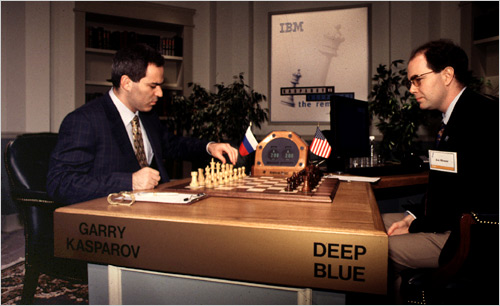
\includegraphics[width=0.8\textwidth]{figs/intro/deep_blue_1.png}

        1997年5月11日,国际象棋世界冠军卡斯帕罗夫与IBM公司的超级电脑深蓝(Deep Blue)对弈。
    \end{column}
    \begin{column}[T]{.5\linewidth}
      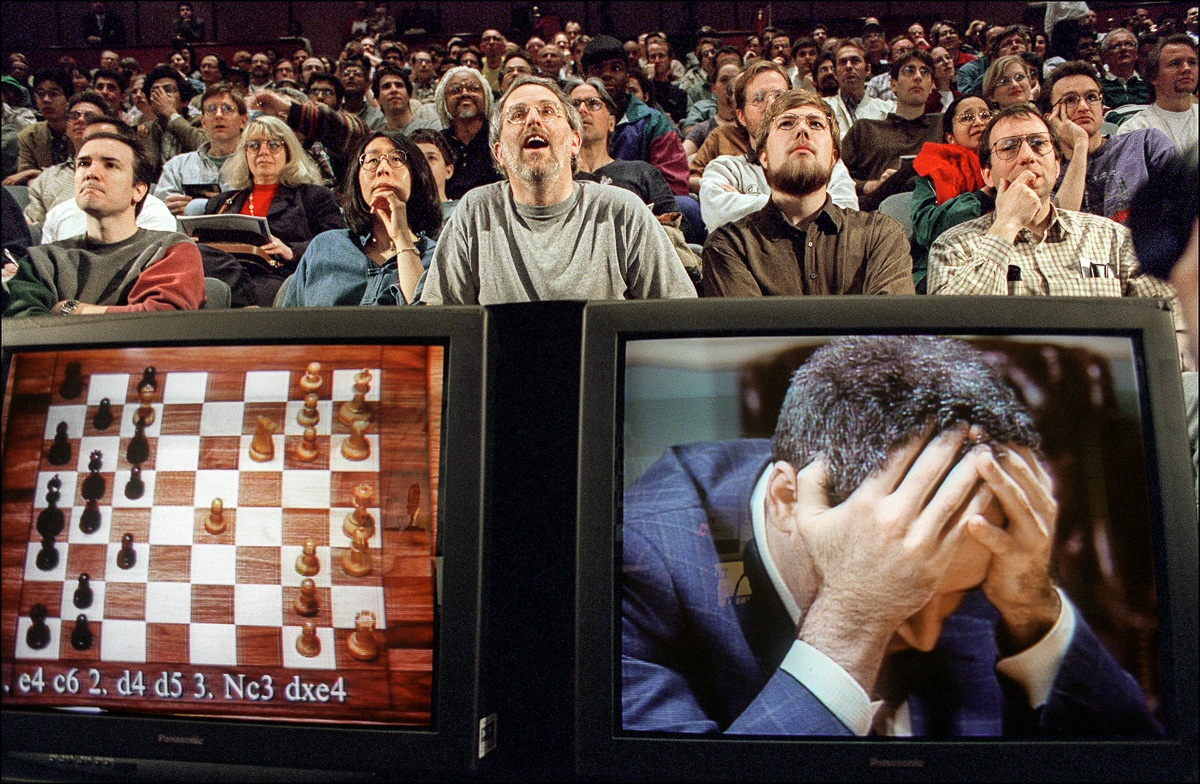
\includegraphics[width=0.8\textwidth]{figs/intro/deep_blue_2.png}

      棋迷在纽约通过电视观战。当日,卡斯帕罗夫在纽约再次负于深蓝,从而在当年的
      “人机大战”中以一胜二负三和的战绩败北。
    \end{column}
  \end{columns}
\end{frame}

\begin{frame}[fragile]
  \frametitle{~}
  \begin{columns}
    \begin{column}[T]{.65\linewidth}
      \begin{enumerate}
      \item 深蓝重量达1.4吨,有32个CPU,每个CPU有8块专门为进行国际象棋对弈设计
        的处理器,平均运算速度为每秒200万步。

        \item 总计256块处理器集成在IBM研制的RS6000/SP并行计算系统中,从而拥有每
          秒超过2亿步的惊人速度。

      \item IBM研制小组向深蓝输入了100年来所有国际特级大师开局和残局的下法。美国
        特级大师本杰明将他对象棋的理解编成程序教给深蓝。虽不会思考,但它无穷无尽
        的计算能力在很大程度上弥补了这一缺陷。
      \end{enumerate}
    \end{column}
    \begin{column}[T]{.3\linewidth}
      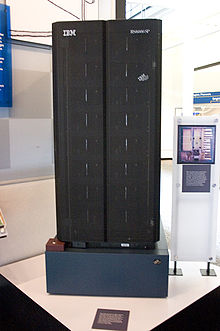
\includegraphics[width=0.8\textwidth]{figs/intro/deep_blue_3.png}
    \end{column}
  \end{columns}
\end{frame}

\begin{frame}[fragile]
  \frametitle{~}
  \begin{columns}
    \begin{column}[T]{.65\linewidth}
      \begin{enumerate}
      \item 模型: 棋盘、棋子的表示
      \item 算法: 对弈的规则和策略
        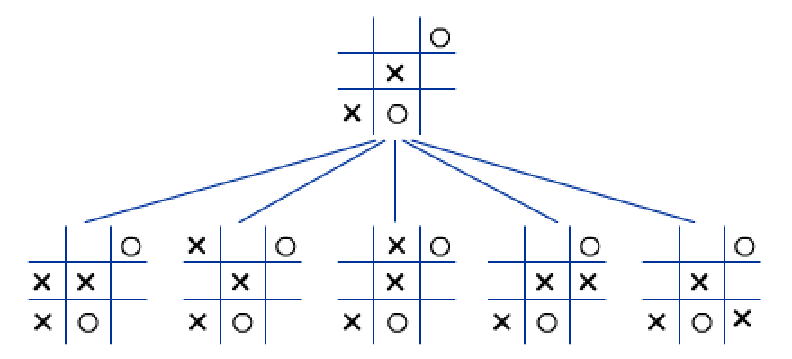
\includegraphics[width=0.8\textwidth]{figs/intro/chess_2.png}
      \item 对弈的本质即在该空间里进行有效的搜索
      \end{enumerate}
    \end{column}
    \begin{column}[T]{.3\linewidth}
      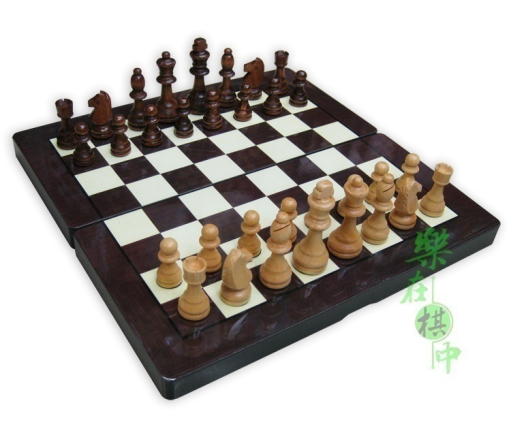
\includegraphics[width=0.8\textwidth]{figs/intro/chess_1.png}
    \end{column}
  \end{columns}
\end{frame}

\begin{frame}[fragile]
  \frametitle{~}

  \begin{columns}
    \begin{column}[T]{.5\linewidth}
      
\includegraphics[width=0.8\textwidth]{figs/intro/alphago_1.png}

      2016年3月9日,Google旗下的AlphaGo电脑击败韩国九段棋手李世石。
    \end{column}
    \begin{column}[T]{.5\linewidth}
      
\includegraphics[width=0.8\textwidth]{figs/intro/alphago_2.png}

      2017年5月27日,世界排名第一的人类棋手柯洁负于AlphaGo,人机大战2.0定格在了0:3。
    \end{column}
  \end{columns}
\end{frame}

\begin{frame}[fragile]
  \frametitle{~}

  \begin{itemize}
  \item 对于擅长于计算的计算机来说,围棋的难度在很大程度上来自于19*19路棋盘背后
    所蕴含的巨大的无法穷尽的变化( 3361种下法),这是基于“穷尽法”的“深蓝”无法在
    围棋上战胜人类的原因。

  \item AlphaGo取得如此成绩,关键是深度学习和类神经网络技术。
  \item AlphaGo将棋盘看作是一个19*19像素构成的图片,利用类似于卷积神经网络的技术
    预测下一步走法。
  \end{itemize}
\end{frame}

\begin{frame}[fragile]
  \frametitle{大语言模型加速技术}
  \begin{easylist}
    & Page Attention
   & Flash Attention
  \end{easylist}

  数据结构与算法的优化,可以解决LLM落地应用的速度问题。
\end{frame}

\begin{frame}[fragile]
  \frametitle{依赖于高效的搜索}
  \begin{easylist}
    & 如何快速的搜索到右方的图例?
  \end{easylist}

    \begin{columns}
    \begin{column}[T]{.6\linewidth}
      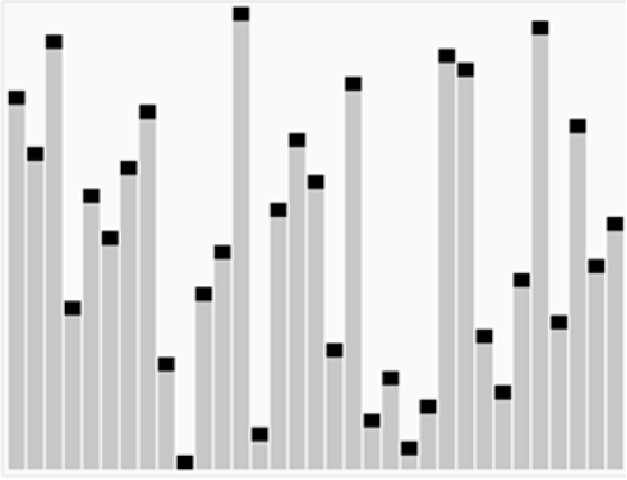
\includegraphics[width=0.8\textwidth]{figs/intro/sort_demo_1.png}
    \end{column}
    \begin{column}[T]{.5\linewidth}
      \vspace{2cm}
      
\includegraphics[width=0.2cm]{figs/intro/sort_demo_2.png}
    \end{column}
  \end{columns}

\end{frame}

\begin{frame}[fragile]
  \frametitle{依赖于高效的搜索}
  \begin{easylist}
    & 如何快速的搜索到右方的图例?
  \end{easylist}

    \begin{columns}
    \begin{column}[T]{.6\linewidth}
      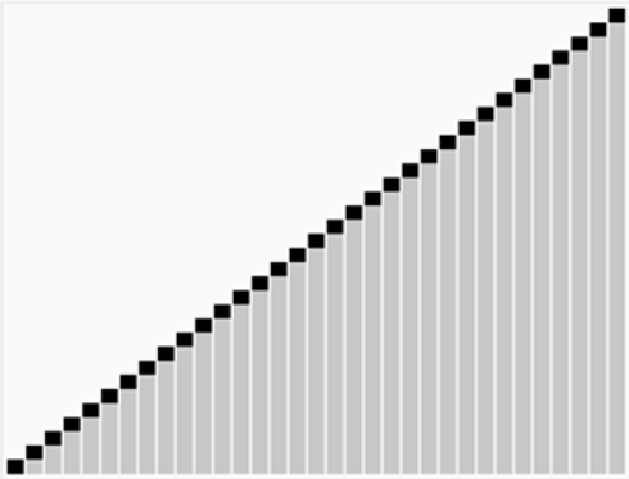
\includegraphics[width=0.8\textwidth]{figs/intro/sort_demo_3.png}
    \end{column}
    \begin{column}[T]{.5\linewidth}
      \vspace{2cm}
      
\includegraphics[width=0.2cm]{figs/intro/sort_demo_2.png}
    \end{column}
  \end{columns}

    数据有序有利于查找。需要对数据进行高效的组织/排序。
\end{frame}

\begin{frame}[fragile]
  \frametitle{Algorithms + Data Structures = Programs}

  \begin{easylist}
    & 算法
    && 处理问题的策略/操作步骤
    & 数据结构
    && 静态数据表示的数学模型(以及必须的操作)
    & 程序
    && 为计算机处理问题编制的一组指令集
  \end{easylist}

  \begin{tcolorbox}[standard jigsaw, opacityback=0, colframe=red]
    数据结构:研究描述现实世界实体的数学模型及其上的操作在计算机中的表示和实现。
  \end{tcolorbox}

\end{frame}

\begin{frame}[fragile]
  \frametitle{FAQ}
  \begin{enumerate}
  \item 数据结构是又一门编程课吗?
  \item 不会C/Java/Python语言怎么办?
  \item 用别的语言学习数据结构可以吗?
  \item 怎样学好数据结构?
  \end{enumerate}
\end{frame}


\subsection{基本概念和术语}
\begin{frame}[fragile]
  \frametitle{基本概念和术语}

  \begin{easylist}
  &  基本概念和术语
  &  抽象数据类型的表示与实现
  &  算法和算法分析
  \end{easylist}
\end{frame}

\begin{frame}[fragile]
  \frametitle{基本概念}

  \begin{easylist}
    & 1、数据 (Data)

    && 对客观事物的符号表示,在计算机科学中特指所有能被输入到计算机中并能被计算
    机程序处理的符号的总称。数据是程序加工的“原料”。

    && 例:一个文字处理程序的处理对象是字符串。

    & 2、数据元素 (Data Element)

    && 数据的基本单位,在计算机程序中通常{\color{red}作为一个整体}被考虑和处理。

    && 例:一本书,一条学生记录。

    && 数据元素可由若干数据项 (Data Item)组成。
  \end{easylist}
\end{frame}

\begin{frame}[fragile]
  \frametitle{基本概念}

  \begin{easylist}
    & 3、数据对象 (Data Object):性质相同的数据元素的集合,是数据的一个子集。

    && 例1: 整数数据对象, $N=\{0, 1, 2, \cdots \}$
    && 例2: 字符数据对象, $C=\{'A', 'B', \cdots \}$

    & 4、数据类型 (Data Type): 一个值的集合和定义在这个值集上的一组操作的总称。

    && 原子类型

    &&& 不可分解的数据类型

    &&& 如:整型、字符型、指针型、空类型…

    && 结构类型

    &&& 可分解为若干成分

    &&& 如:数组由分量组成,分量可以是整型,也可以是数组.
  \end{easylist}
\end{frame}

\begin{frame}[fragile]
  \begin{tcolorbox}[colframe=red, title=数据结构]
      数据结构 (狭义上) 是相互之间存在一种或多种特定关系的数据元素的集合。
  \end{tcolorbox}

  \begin{easylist}
    & 逻辑结构
    && 集合、线性结构、树形结构、图状或网状结构

    & 物理结构:数据结构在计算机中的表示/映像
    && 数据元素的表示是结点 (node),即在计算机内用若干位组合起来表示一个数据元素。
    && 数据关系的表示有顺序映像和非顺序映像两种,由此得到顺序存储结构和链式存储结构。
  \end{easylist}
\end{frame}

\begin{frame}[fragile]
  \frametitle{物理结构}
  \begin{easylist}
    & 顺序映像 (顺序存储结构)

    && 逻辑上相邻的数据元素存储在物理位置上相邻的存储单元中比如在高级语言中的“一
    维数组”。

    & 非顺序映像 (链式存储结构)

    && 数据元素可以存储在计算机内任意位置上,它们的逻辑关系用指针来链接。比如在
    高级语言中的“指针”。
  \end{easylist}
\end{frame}

\begin{frame}[fragile]
  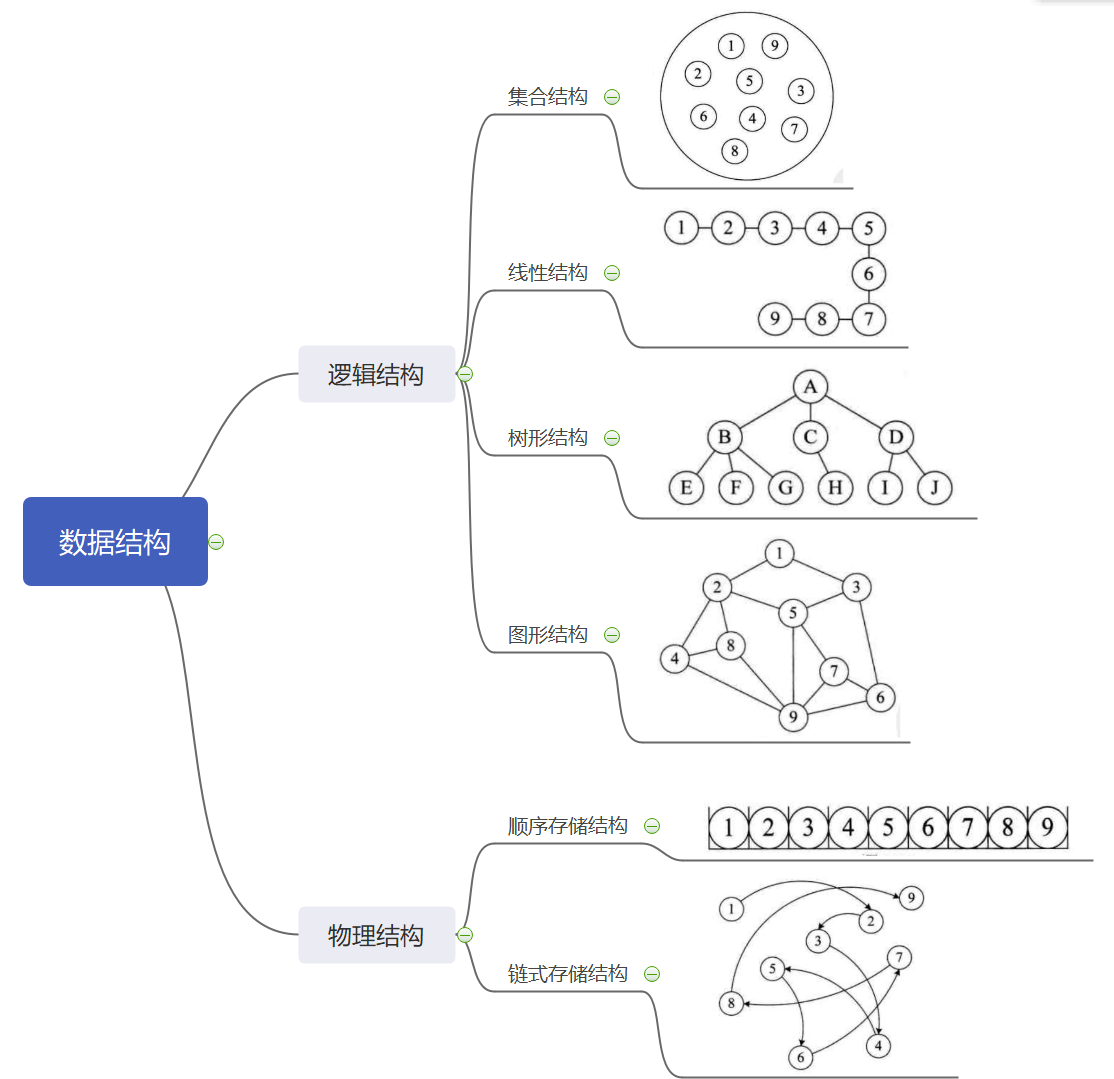
\includegraphics[width=0.7\textwidth]{figs/intro/ds_category.png}
\end{frame}


\subsection{抽象数据类型的表示和实现}
\begin{frame}[fragile]
  \frametitle{抽象数据类型的表示和实现}
  \begin{easylist}
    & 抽象数据类型 (Abstract Data Type)是指一个数学模型以及定义在该模型上的一组操作。

    && 例如,矩阵 +(求转置、加、乘、求逆、求特征值)构成一个矩阵的抽象数据类型

    &&“抽象”在于数据类型的数学抽象特性,与具体表示和实现无关。
  \end{easylist}
\end{frame}

\begin{frame}[fragile]
  \frametitle{抽象数据类型的示例}
  \scriptsize
  \begin{minted}{c}
ADT Complex {
   数据对象:D = {e1,e2 | e1,e2 in RealSet  }
   数据关系:R1 = {<e1,e2> | e1是复数的实数部分,  e2 是复数的虚数部分 }
   基本操作:
       InitComplex( &Z, v1, v2 )
          操作结果:构造复数Z,实部和虚部分别被赋以参数v1和v2的值.
      DestroyComplex( &Z)
          操作结果:复数Z被销毁.
      GetReal( Z, &realPart )
          初始条件:复数已存在。
          操作结果:用realPart返回复数Z的实部值.
     GetImag( Z, &ImagPart )
          初始条件:复数已存在。
          操作结果:用ImagPart返回复数Z的虚部值.
     Add( z1,z2, &sum )
          初始条件:z1,z2是复数。
          操作结果:用sum返回两个复数z1,z2的和值.
} ADT Complex
  \end{minted}
\end{frame}

\subsection{算法和算法分析}
\begin{frame}[fragile]
  \frametitle{算法和算法分析}
  \begin{itemize}
  \item 基本概念和术语
  \item 抽象数据类型的表示与实现
  \item 算法和算法分析
  \end{itemize}
\end{frame}

\begin{frame}[fragile]
  \frametitle{Alkhwarizmi与Algorithm}
  \begin{itemize}
  \item Alkhwarizmi(约780~约850),数学家,代数与算术的整理者。阿拉伯文
    Alkhwarizmi 原意是来自 (al-) 花剌子模 (Khwarizmi) 。
  \item Alkhwarizmi在当时的学问中心巴格达,服务于宫廷。他写了一本有关代数的书,
    这本书转成欧文,书名逐渐简化为algebra(代数)。
  \item 后来Alkhwarizmi又引进了印度数字发展算术,后经 Fibonacci(1170~1250年)
    引入欧洲。欧洲人把 Alkhwarizmi这个字拉丁化,称用十进位印度阿拉伯数字来进行有
    规则可寻的计算的算术为 Algorithm。后来算术转用其它的字(如 arithmetic), 而
    algorithm 则成为计算机科学的行话。
  \end{itemize}
\end{frame}

\begin{frame}[fragile]
  \frametitle{算 法 (Algorithm) }
  \begin{easylist}
    & 算法是对特定问题求解步骤的一种描述,是指令的有限序列,其中每一条指令表示一
    个或多个操作。算法可以看做是从输入到输出的一个映射。

    && Input $\rightarrow$ Ouput

    & 算法的描述

    && 自然语言

    && 程序流程图

    && 伪码: 它忽略高级程序设计语言中一些严格的语法规则与描述细节,因此比程序设
    计语言更容易描述和被人理解,而比自然语言更接近程序设计语言。它虽然不能直接执
    行但很容易被转换成高级语言。

    && 编程语言
  \end{easylist}
\end{frame}

\begin{frame}[fragile]
  \frametitle{试写出[9,2,5,1,6,7,10]经过下列程序处理后的序列。}

  \begin{minted}{c}
//冒泡法
void bubble (int a[], int n) {
  for (i=n-1; i>=1; i - -) {
    for (j=0; j<i; j++)
      if (a[j]>a[j+1]) {
        swap(&a[j],&a[j+1]);
      }
  }
}
  \end{minted}

  \begin{easylist}
    & $i = n - 1 $ $\cdots$

    & $i = n - 2 $ $\cdots$
  \end{easylist}
\end{frame}

\begin{frame}[fragile]
  \frametitle{算法设计的要求}
  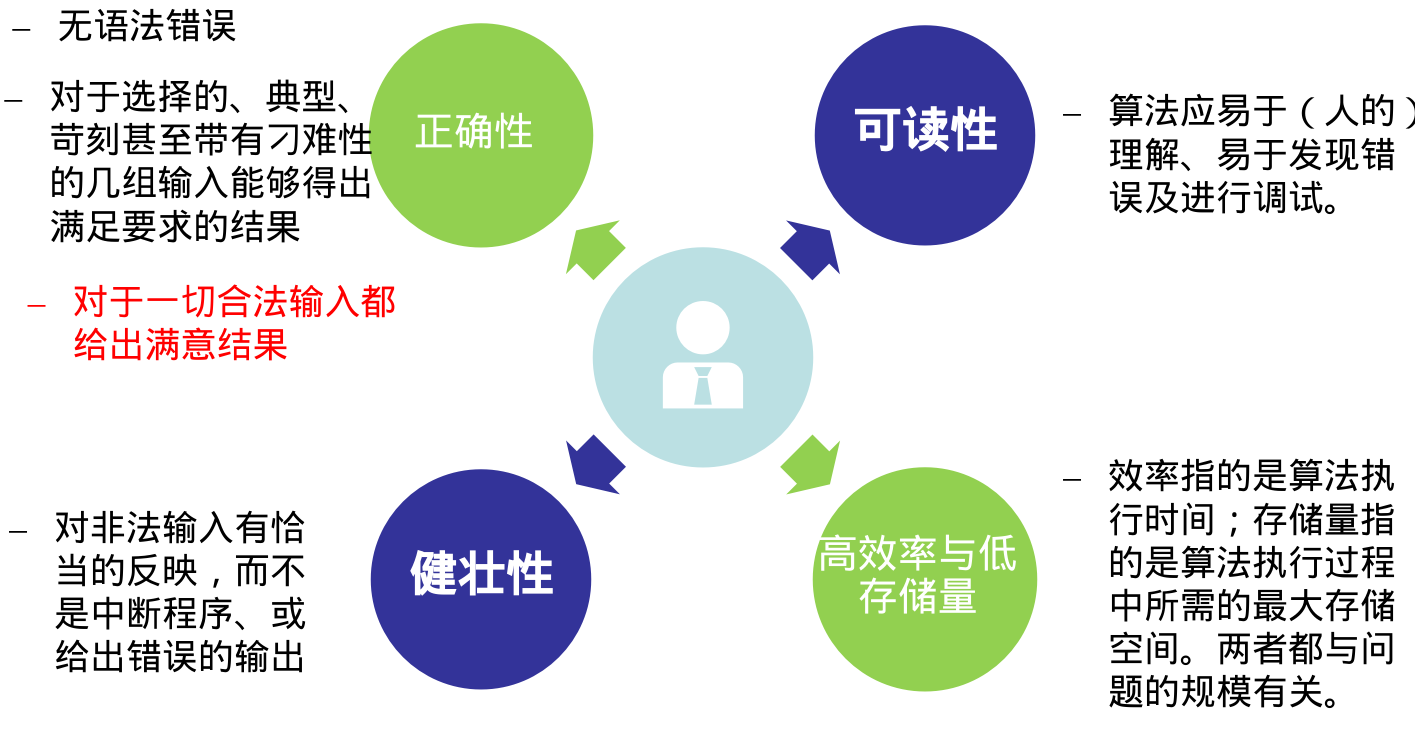
\includegraphics[width=0.9\textwidth]{figs/intro/algorithm_req.png}
\end{frame}

\begin{frame}[fragile]
  \frametitle{算法效率}
  \begin{easylist}
    & 算法执行时间需通过依据该算法编制的程序在计算机上运行时所消耗的时间来度量。

    & 相关影响因素包括:

    && 机器硬件配置直接影响计算机执行指令的速度
    && 编写程序的语言:越高级, 效率越低
    && 算法选用的策略
    && 问题的规模:规模越大, 耗时越久
    && 编译程序产生的机器代码的质量
  \end{easylist}
\end{frame}

\begin{frame}[fragile]
  \frametitle{快递员配送包裹}
  \begin{easylist}
    & 假定快递员以恒定速度行驶,比较下面的方案

    && 方案1:配送n个包裹的总时间为$n^2 + n$

    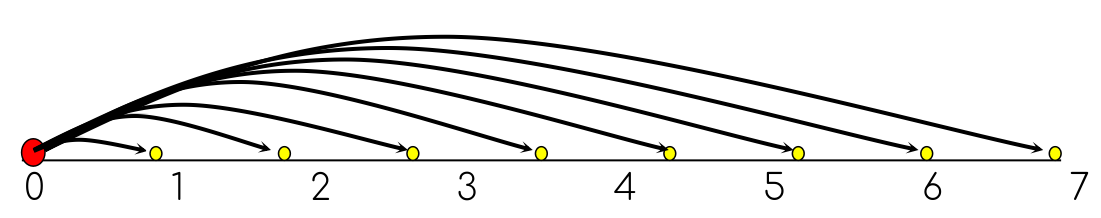
\includegraphics[width=0.8\textwidth]{figs/intro/postman1.png}

    && 方案2:配送n个包裹的总时间为2n

    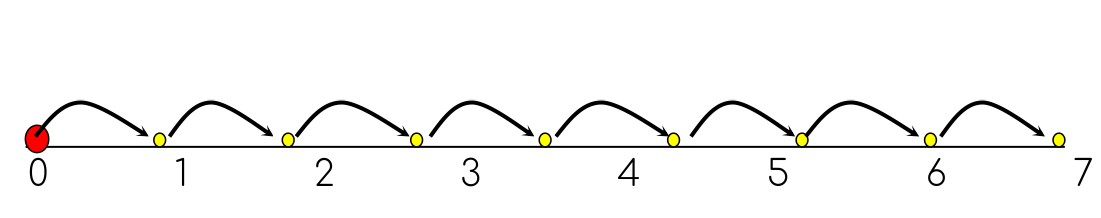
\includegraphics[width=0.8\textwidth]{figs/intro/postman2.png}
  \end{easylist}
\end{frame}

\begin{frame}[fragile]
  \frametitle{各函数的增长率}
  在问题规模增长时,算法执行时间必定也会增长。我们关心的是这个执行次数以什么样的数量级(增长率)增长。

  \begin{center}
    \begin{tabular}{| r | r | r | r | r |}
      \hline
      $n$ & $long_2{n}$ & $n \cdot log_2 n$ & $n^2$ & $2^n$ \\ \hline
      1 & 0 & 0 & 1 & 2 \\ \hline
      2 & 1 & 2 & 2 & 4 \\ \hline
      4 & 2 & 8 & 16 & 16 \\ \hline
      8 & 3 & 24 & 64 & 256 \\ \hline
      16 & 4 & 64 & 256 & 65,536  \\ \hline
      32 & 5 & 160 & 1,024 & 4,294,967,296  \\ \hline
    \end{tabular}
  \end{center}
\end{frame}

\begin{frame}[fragile]
  \frametitle{观察$g(n)$和$f(n)$的相对增长趋势}

  \begin{center}
    \begin{tabular}{| r | r | r |}
      \hline
      $n$ & $g(n)=n^2$ & $f(n)=n^2+4n+20$ \\ \hline
      10 & 300 & 360  \\ \hline
      50 & 2,500 & 2,720  \\ \hline
      100 & 10,000 & 10,420  \\ \hline
      1,000 & 1,000,000 & 1,004,020  \\ \hline
      10,000 & 100,000,000 & 100,040,020  \\ \hline
    \end{tabular}
  \end{center}

  \begin{easylist}
    & 当n变得很大时,$n^2$成为主导项,通过$g(n)$的变化情况就可以预测$f(n)$的变化。

    \[O(c_1 n^k + c_2 n^{k-1} + \cdots + c_k) = O(n^k)\]

    & 例如,$T(n)=3n^ 2+ 4n + 20$,记为$O(n^2)$
  \end{easylist}
\end{frame}

\begin{frame}[fragile]
  \frametitle{Big-O Complexity Chart}
  \begin{columns}
    \begin{column}[T]{.6\linewidth}            %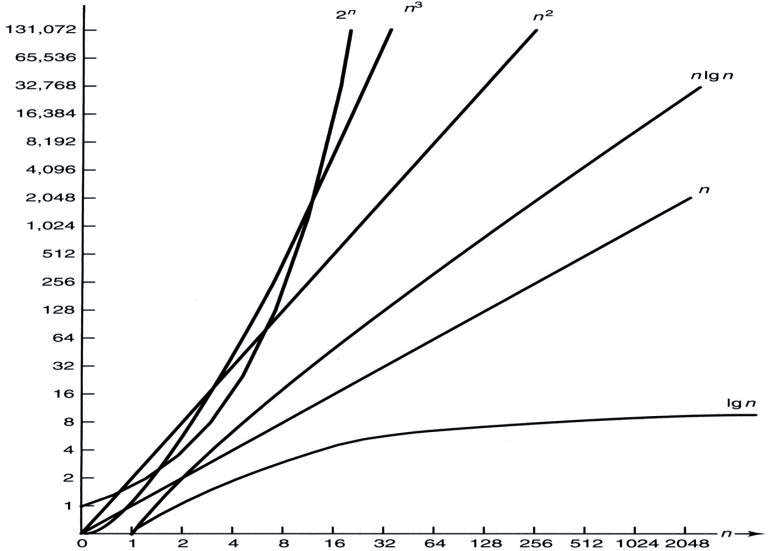
\includegraphics[width=1.0\textwidth]{figs/intro/Growth-Rates-of-Some-Common-Complexity-Functions.png}
        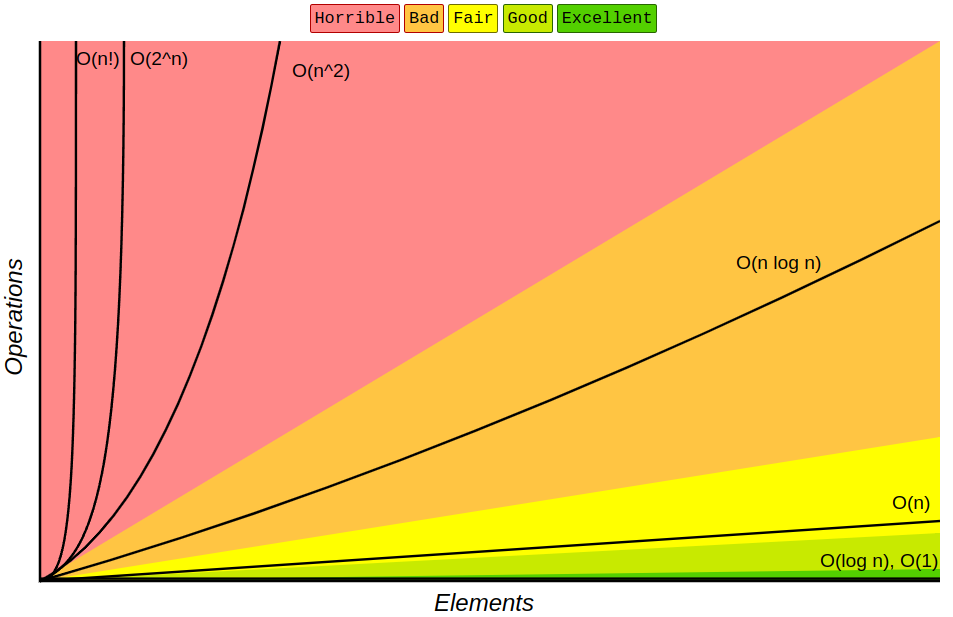
\includegraphics[width=1.0\textwidth]{figs/intro/bigocheatsheet.png}

        From: \url{https://www.bigocheatsheet.com}
    \end{column}
    \begin{column}[T]{.4\linewidth}
      \scriptsize
      From better to worse:

      \begin{tabular}{l l}
        \hline
        $O(1)$ & constant time \\ \hline
        $O(\log n)$ & log time \\ \hline
        $O(n)$ & linear time \\ \hline
        $O(n \log n)$ & log linear time \\ \hline
        $O(n^2)$ & quadratic time \\ \hline
        $O(n^3)$ & cubic time \\ \hline
        $O(2^n)$ & exponential time \\ \hline
      \end{tabular}
    \end{column}
  \end{columns}
\end{frame}

\begin{frame}[fragile]
  \frametitle{大O表示法}
  \begin{easylist}
    & 算法的(渐近)时间复杂度记作: $T(n) = O(f(n))$

    && 表示随问题规模$n$的增大,算法执行时间的增长率和$f(n)$的增长率相同。

    & 通常是从算法中选取一种最基本的元操作,以该操作重复执行的次数(频度)来度量算法效率
  \end{easylist}
\end{frame}

\begin{frame}[fragile]
  \frametitle{例:矩阵相乘 (C代码示例)}
  \begin{minted}{c}
    for (i=1; i<=n; i++)
      for (j=1; j<=n; j++) {
        c[i][j] = 0;
        for (k=1; k<=n; k++)
          c[i][j] =c[i][j]+ a[i][k] * b[k][j]; // 该语句可看作元操作
      }
  \end{minted}

  \begin{tcolorbox}
    整个算法的执行时间与元操作重复执行的次数$n^3$成正比,记作$T(n) = O(n^3)$
  \end{tcolorbox}
\end{frame}

\begin{frame}[fragile]
  \frametitle{例:矩阵相乘 (Python代码示例)}
  \begin{minted}{python}
n = 3
a = [[1,2,3],[4,5,6], [7,8,9]]
b = [[1,2,3],[4,5,6], [7,8,9]]

c = [ [0]*n for _ in range(n) ]
for i in range(n):
    for j in range(n):
        c[i][j] = 0
        for k in range(n):
            c[i][j] = c[i][j] + a[i][k] * b[k][j]
  \end{minted}

  \begin{tcolorbox}
    整个算法的执行时间与元操作重复执行的次数$n^3$成正比,记作$T(n) = O(n^3)$
  \end{tcolorbox}
\end{frame}

\begin{frame}[fragile]
  \frametitle{请观察 [10,9,7,6] 和 [6,7,9,10]在处理上的不同。}
  \begin{minted}{c}
    void bubble(int a[], int n) {
      for (i=n-1; i>=1; i - -) {
        for (j=0; j<i; j++)
          if (a[j]>a[j+1]) {
              swap(&a[j],&a[j+1]);
          }
      }
    }
  \end{minted}

  \pause

  \begin{itemize}
  \item 若初始文件是正序的,一趟扫描即可完成排序。
  \item 若初始文件是反序的,需要进行$n-1$趟排序。
  \item \color{red}计算平均复杂度,或最坏情况下的时间复杂度.
  \end{itemize}
\end{frame}

\begin{frame}[fragile]
  \frametitle{~}
  \begin{itemize}
    \item 最好情况的时间复杂度 (初始文件是正序的)

      [6,7,9,10] --- 一趟扫描即可完成排序,共计$n-1$次比较(0次交换)。

      冒泡排序最好情况的时间复杂度为$O(n)$

   \item 最坏情况的时间复杂度 (初始文件是反序的)

     [10,9,7,6] --- 需要进行n-1趟扫描,每趟进行$i$次比较+交换$(1\leq i \leq n-1)$ ,共计$\dfrac{n (n-1)}{2}$次比较+交换。

     冒泡排序的最坏情况的时间复杂度为$O(n^2)$

  \end{itemize}
\end{frame}

\begin{frame}[fragile]
  \frametitle{算法的存储空间需求 (内存)}
  \begin{easylist}
    & 算法需要为: 输入数据、程序、辅助变量提供存储空间。
    & 算法的空间复杂度: $S(n) = O(g(n))$
    & 随着问题规模增大,算法运行所需存储量的增长率与$g(n)$的增长率相同。
    & 若所需存储量依赖于特定的输入,则通常按最坏情况考虑。
    & 相对于时间复杂度而言,空间复杂度在很多时候不需进行分析。
  \end{easylist}
\end{frame}

\begin{frame}[fragile]
  \frametitle{小结}

  \begin{enumerate}
  \item 数据结构 研究非数值计算的程序设计问题中计算机的操作对象以及它们之间的关系和操作。
  \item 数据、数据元素、数据对象、数据结构的概念
  \item 常见的基本数据结构
  \item 以大O表示法分析算法时间复杂度
  \end{enumerate}
\end{frame}

%\section{线性表 (Linear  List)}

\begin{frame}[fragile]
  \frametitle{线性表 --- Linear  List}
  \begin{enumerate}
  \item 基本概念
  \item 顺序表
  \item 链表
  \end{enumerate}
\end{frame}

\subsection{线性表概述}
\begin{frame}[fragile]
  \frametitle{线性表}

  \begin{easylist}
    & 线性表举例:
    && 英文字母表 $A, B, C, \cdots, Z$
    && 某单位近5年的计算机数量 $(40, 60, 100, 150, 180)$
    && 某产品淘宝的销售记录.
    
    & 特点
    && 数据元素是多样的,但具有相同特性
    && 相邻元素之间有序偶关系<前驱, 后继>    
  \end{easylist}
\end{frame}

\begin{frame}[fragile]
  \frametitle{线性表}

  \begin{tcolorbox}[standard jigsaw, opacityback=0, colframe=red, title=线性表是n个数据元素的有限序列]
    \[
    (a_1, a_2, \cdots, a_i, \cdots, a_n)
    \]
  \end{tcolorbox}

  \begin{itemize}
  \item 存在唯一的{\color{red}第一个}数据元素,存在唯一的的{\color{red}最后一个}数据元素。
  \item 除第一个之外,每个数据元素只有一个前驱;除最后一个之外,每个数据元素只有
    一个后继。
  \item 线性表的长度:线性表中元素的个数,常记作length, len, n. 当空表时,len=0.
  \end{itemize}
\end{frame}

\begin{frame}[fragile]
  \frametitle{线性表的两种存储方式}
  \begin{enumerate}
  \item 方案1:顺序存储 --- 称顺序表
  \item 方案2:链式存储 --- 称链表
  \end{enumerate}
\end{frame}


\subsection{顺序表}
\begin{frame}[fragile]
  \frametitle{方案1: 顺序表 (Sequence List)}
  \begin{columns}
    \begin{column}[T]{.5\linewidth}
      \[
      (a_1, a_2, \cdots, a_i, \cdots, a_n)
      \]
      \begin{easylist}
        & 建一个数组, 用一组地址连续的存储单元依次存储数据元素。

        && 逻辑上相邻的数据元素,其物理存储位置也相邻

      \end{easylist}
    \end{column}
    \begin{column}[T]{.5\linewidth}
      \begin{tcolorbox}[]
        \scalebox{0.7}{
          \begin{tikzpicture}[scale=0.5, box/.style={draw, minimum width=1.2cm, minimum height=0.5cm, fill=yellow!10}]
	          \draw node[box] (a1) {$a_1$}
	          node[box, below=0 of a1] (a2) {$a_2$}
	          node[box, below=0 of a2] (a3) {$\cdots$}
	          node[box, below=0 of a3] (ai) {$a_i$}
	          node[box, below=0 of ai] (a5) {$\cdots$}
	          node[box, below=0 of a5] (an) {$a_n$}
	          node[box, below=0 of an, fill=gray!30] (a7) {}
	          node[box, below=0 of a7, fill=gray!30] (a8) {}
	          node[box, below=0 of a8, fill=gray!30] (a9) {};

	          \draw node[right=0.3 of a1] (p1) {$1$}
	          node[right=0.3 of a2] (p2) {$2$}
	          node[right=0.3 of ai] (pi) {$i$}
	          node[right=0.3 of an] (pn) {$n$}
	          node[right=0.3 of a7] (p7) {空闲}
	          node[right=0.3 of a8] (p8) {空闲}
	          node[right=0.3 of a9] (p9) {空闲};

	          \draw node[left=0.3 of a1] (p1) {$b$}
	          node[left=0.3 of a2] (p2) {$b+l$}
	          node[left=0.3 of ai] (pi) {$b+(i-1)\cdot l$}
	          node[left=0.3 of an] (pn) {$b+(n-1)\cdot l$}
	          node[left=0.3 of a7] (p7) {$b+n\cdot l$}
	          node[left=0.3 of a8] (p8) {$\cdots$}
	          node[left=0.3 of a9] (p9) {$b+(MaxLen-1)\cdot l$};

	          \draw node[above left=0.3 of p1] (tip) {起始地址/基地址};
	          \draw[draw=red, thick, -Latex] (tip) -> (p1);
          \end{tikzpicture}
        }
      \end{tcolorbox}
    \end{column}
  \end{columns}
\end{frame}

\begin{frame}[fragile]
  \frametitle{顺序表 (Sequence List)}
  \begin{columns}
    \begin{column}[T]{.5\linewidth}
      \begin{easylist}
        & 为便于维护处理,记录3个变量

        && 存放表元素的数组list;
        && 表的长度length;
        && 存储容量maxSize;

        & 常用的基本操作
        && 判断是否空: isEmpty()
        && 求长度: length()
        && 取元素: get(i)
        && 插入操作: insert(i,x)
        && 删除操作: remove(i)
        && 查找: indexOf(x)
        && 输出: display()
      \end{easylist}
    \end{column}
    \begin{column}[T]{.5\linewidth}
      \begin{tcolorbox}[]
        \scalebox{0.7}{
          \begin{tikzpicture}[scale=0.5, box/.style={draw, minimum width=1.2cm, minimum height=0.5cm, fill=yellow!10}]
	          \draw node[box] (a1) {$a_1$}
	          node[box, below=0 of a1] (a2) {$a_2$}
	          node[box, below=0 of a2] (a3) {$\cdots$}
	          node[box, below=0 of a3] (ai) {$a_i$}
	          node[box, below=0 of ai] (a5) {$\cdots$}
	          node[box, below=0 of a5] (an) {$a_n$}
	          node[box, below=0 of an, fill=gray!30] (a7) {}
	          node[box, below=0 of a7, fill=gray!30] (a8) {}
	          node[box, below=0 of a8, fill=gray!30] (a9) {};

	          \draw node[right=0.3 of a1] (p1) {$1$}
	          node[right=0.3 of a2] (p2) {$2$}
	          node[right=0.3 of ai] (pi) {$i$}
	          node[right=0.3 of an] (pn) {$n$}
	          node[right=0.3 of a7] (p7) {空闲}
	          node[right=0.3 of a8] (p8) {空闲}
	          node[right=0.3 of a9] (p9) {空闲};

	          \draw node[left=0.3 of a1] (p1) {$b$}
	          node[left=0.3 of a2] (p2) {$b+l$}
	          node[left=0.3 of ai] (pi) {$b+(i-1)\cdot l$}
	          node[left=0.3 of an] (pn) {$b+(n-1)\cdot l$}
	          node[left=0.3 of a7] (p7) {$b+n\cdot l$}
	          node[left=0.3 of a8] (p8) {$\cdots$}
	          node[left=0.3 of a9] (p9) {$b+(MaxLen-1)\cdot l$};
          \end{tikzpicture}
        }
      \end{tcolorbox}
    \end{column}
  \end{columns}
\end{frame}

\begin{frame}[fragile]
  \frametitle{补充:常用命名规则之驼峰与蛇形命名法}
  \begin{center}
    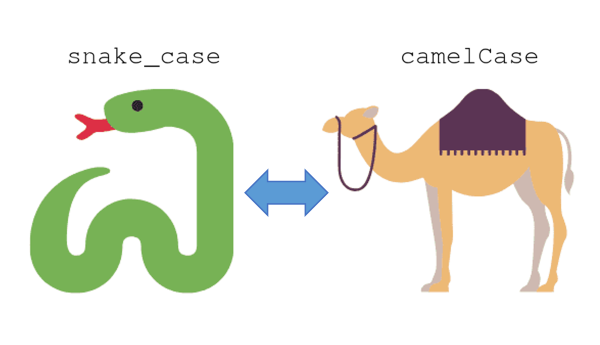
\includegraphics[width=0.5\textwidth]{figs/list/snake_case_camel_case.png}
    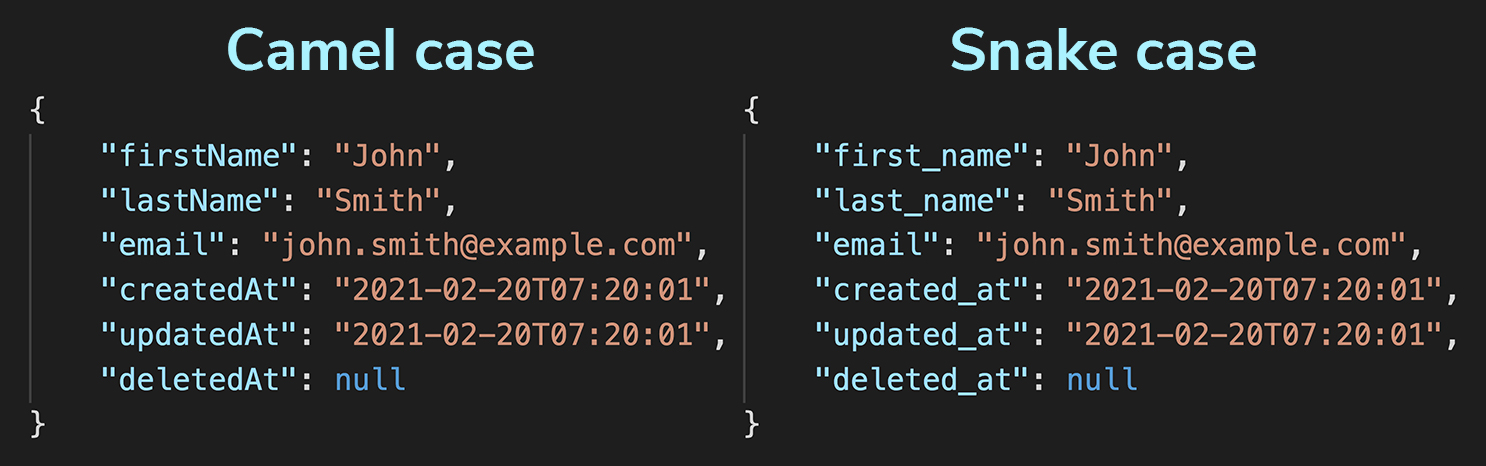
\includegraphics[width=0.85\textwidth]{figs/list/snake_vs_camel.jpg}
  \end{center}
\end{frame}

\begin{frame}[fragile]
  %\frametitle{线性表}
  \begin{minted}{java}
public class SequenceList {
    int maxSize; //最大长度
    int length; //当前长度
    Elem[] list; //对象数组

    public bool isEmpty()
    public int length()
    public Elem get(i) throws Exception
    public void insert(i,e)
    public void remove(i) throws Exception
    public int indexOf(e)
    public void display()
    public void clear()
}
  \end{minted}
\end{frame}

\begin{frame}[fragile]
  %\frametitle{线性表}
  \begin{minted}{python}
class SequenceList:
    def __init__(self, max_size, elements):
        self.max_size = max_size
        self.length = len(elements)
        self.elements = [0]*max_size
        for idx, value in enumerate(elements):
            self.elements[idx] = value

    def __len__(self):
        return self.length

    def __getitem__(self, i):
        return self.elements[i]

    def __setitem__(self, i, value):
        self.elements[i] = value

    def __delitem__(self, i):
        del self.elements[i]
        self.length = self.length - 1
  \end{minted}
\end{frame}

\begin{frame}[fragile]
  \frametitle{初始化顺序表}
  Java/C Example

  \begin{minted}{java}
//初始化空表
void initList(int size) {
    list = new Elem[size];
    maxSize = size; //初始存储容量
    length = 0; //空表长度为0
}
  \end{minted}

  Python Example:

  \begin{minted}{python}
    self.elements = [0]*max_size
  \end{minted}
\end{frame}

\begin{frame}[fragile]
  \frametitle{在index位置上插入元素e}
  \begin{minted}{java}
boolean insert(int index, Elem e) {
  if (length== maxSize)    //当前线性表已满
     {print("顺序表已满!");  return false;}
  if (index < 0 || index > length)    //插入位置编号不合法
    {print("参数错误!");  return false;}

  for (int j = length- 1; j >= index; j--)   //向后移动元素
     list[j + 1] = list[j];

  list[index] = e;    //插入元素
  length ++;
  return true;
}
  \end{minted}
\end{frame}


\begin{frame}[fragile]
  \frametitle{插入元素的时间复杂度}

  \scalebox{0.75} {
    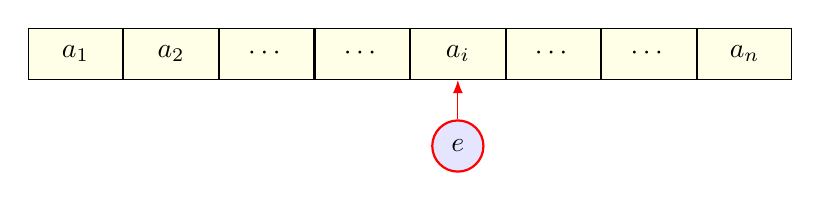
\begin{tikzpicture}[box/.style={draw, minimum width=1.2cm, minimum height=0.65cm, fill=yellow!10}]
	    \draw node[box] (a1) {$a_1$}
	    node[box, right=0 of a1] (a2) {$a_2$}
	    node[box, right=0 of a2] (a3) {$\cdots$}
	    node[box, right=0 of a3] (a4) {$\cdots$}
	    node[box, right=0 of a4] (ai) {$a_i$}
	    node[box, right=0 of ai] (a6) {$\cdots$}
	    node[box, right=0 of a6] (a7) {$\cdots$}
	    node[box, right=0 of a7] (an) {$a_n$}
		  node[draw=red, ellipse, minimum width=0.65cm, minimum height=0.65cm, thick, fill=blue!10, below=0.5 of ai] (cur) {$e$};
		  \draw[draw = red, -Latex] (cur) -- (ai);
    \end{tikzpicture}
  }

  \begin{easylist}
    & 在长为n的线性表中插入一个元素,所需移动元素次数的平均次数为?

    && 有多少种可能的插入位置?$n+1$

    && 假设这些位置以同等概率出现,每个概率$\dfrac{1}{n+1}$。每个情形下分别移动
    $n, n-1, \cdots, 0$次。求加权和为$n/2$。

    && 平均时间复杂度:$T(n)=O(n)$
  \end{easylist}
\end{frame}

\begin{frame}[fragile]
  \frametitle{删除index位置上的元素}
  \scalebox{0.7}{
    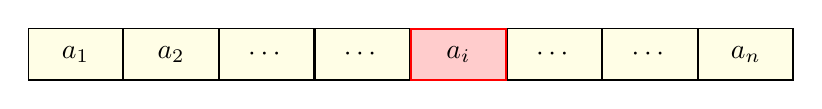
\begin{tikzpicture}[scale=0.5, box/.style={draw, minimum width=1.2cm, minimum height=0.65cm, fill=yellow!10}]
	    \draw node[box] (a1) {$a_1$}
	    node[box, right=0 of a1] (a2) {$a_2$}
	    node[box, right=0 of a2] (a3) {$\cdots$}
	    node[box, right=0 of a3] (a4) {$\cdots$}
	    node[box, draw=red, thick, fill=red!20, right=0 of a4] (ai) {$a_i$}
	    node[box, right=0 of ai] (a6) {$\cdots$}
	    node[box, right=0 of a6] (a7) {$\cdots$}
	    node[box, right=0 of a7] (an) {$a_n$};
    \end{tikzpicture}
  }

  \begin{minted}{java}
boolean remove(int index) {
    if(index<0||index>=length)  
          return false;
    if(getLength()==0)
          return false;
    for (int j=index;j<length-1; j++)    //前移
          Elem[j]=elem[j+1];
    length--;
}
  \end{minted}
\end{frame}

\begin{frame}[fragile]
  \frametitle{删除元素的时间复杂度}
  \scalebox{0.7}{
    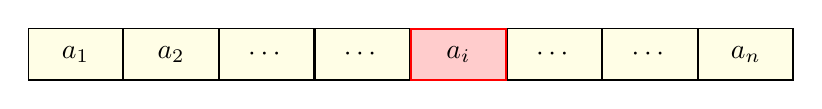
\begin{tikzpicture}[scale=0.5, box/.style={draw, minimum width=1.2cm, minimum height=0.65cm, fill=yellow!10}]
	    \draw node[box] (a1) {$a_1$}
	    node[box, right=0 of a1] (a2) {$a_2$}
	    node[box, right=0 of a2] (a3) {$\cdots$}
	    node[box, right=0 of a3] (a4) {$\cdots$}
	    node[box, draw=red, thick, fill=red!20, right=0 of a4] (ai) {$a_i$}
	    node[box, right=0 of ai] (a6) {$\cdots$}
	    node[box, right=0 of a6] (a7) {$\cdots$}
	    node[box, right=0 of a7] (an) {$a_n$};
    \end{tikzpicture}
  }

  \begin{itemize}
  \item 在长度为n的线性表中删除一个元素:
    \begin{itemize}
    \item 共有n个可能的位置,每个有1/n的概率。每个情形下分别移动n-1, …, 0次。求加权和为(n-1)/2。
    \item $T(n)=O(n)$
    \end{itemize}
  \end{itemize}

  \pause

  \begin{tcolorbox}[standard jigsaw, opacityback=0, colframe=red, title=结论]
    在顺序表中插入或删除一个元素时,平均移动一半元素,当$n$很大时,效率很低.
  \end{tcolorbox}
\end{frame}

\begin{frame}[fragile]
  \frametitle{顺序表特点:地址连续}
  \begin{columns}
    \begin{column}[T]{.5\linewidth}
      \begin{tcolorbox}[]
      \scalebox{0.7}{
        \begin{tikzpicture}[scale=0.5, box/.style={draw, minimum width=1.2cm, minimum height=0.5cm, fill=yellow!10}]
	        \draw node[box] (a1) {$a_1$}
	        node[box, below=0 of a1] (a2) {$a_2$}
	        node[box, below=0 of a2] (a3) {$\cdots$}
	        node[box, below=0 of a3] (ai) {$a_i$}
	        node[box, below=0 of ai] (a5) {$\cdots$}
	        node[box, below=0 of a5] (an) {$a_n$}
	        node[box, below=0 of an, fill=gray!30] (a7) {}
	        node[box, below=0 of a7, fill=gray!30] (a8) {}
	        node[box, below=0 of a8, fill=gray!30] (a9) {};

	        \draw node[right=0.3 of a1] (p1) {$1$}
	        node[right=0.3 of a2] (p2) {$2$}
	        node[right=0.3 of ai] (pi) {$i$}
	        node[right=0.3 of an] (pn) {$n$}
	        node[right=0.3 of a7] (p7) {空闲}
	        node[right=0.3 of a8] (p8) {空闲}
	        node[right=0.3 of a9] (p9) {空闲};

	        \draw node[left=0.3 of a1] (p1) {$b$}
	        node[left=0.3 of a2] (p2) {$b+l$}
	        node[left=0.3 of ai] (pi) {$b+(i-1)\cdot l$}
	        node[left=0.3 of an] (pn) {$b+(n-1)\cdot l$}
	        node[left=0.3 of a7] (p7) {$b+n\cdot l$}
	        node[left=0.3 of a8] (p8) {$\cdots$}
	        node[left=0.3 of a9] (p9) {$b+(MaxLen-1)\cdot l$};
        \end{tikzpicture}
      }
      \end{tcolorbox}
    \end{column}
    \begin{column}[T]{.5\linewidth}
      \begin{easylist}
        & 优点
        && 直观
        && 随机存储效率高
        \pause
        & 缺点
        && 移动元素代价大
      \end{easylist}
    \end{column}
  \end{columns}
\end{frame}


\subsection{链表}
\begin{frame}[fragile]
  \frametitle{方案2: 链式存储---链表}
  \begin{columns}
    \begin{column}[T]{.4\linewidth}
      \scalebox{0.5}{    \begin{tikzpicture}[fill=red, box/.style={draw, minimum width=2cm, minimum height=0.85cm, fill=yellow!10}]
	      \draw node[box] (dh) {数据域}  node[box, right=0 of dh] (ph) {指针域}
	 node[box, below=0.5 of dh] (d_li) {LI}  node[box, right=0 of d_li] (p_li) {43} node[left=0.2 of d_li] {1}
	 node[box, below=0.5 of d_li] (d_qian) {QIAN}  node[box, right=0 of d_qian] (p_qian) {13} node[left=0.2 of d_qian] {7}
	 node[box, below=0.5 of d_qian] (d_sun) {SUN}  node[box, right=0 of d_sun] (p_sun) {1} node[left=0.2 of d_sun] {13}
	 node[box, below=0.5 of d_sun] (d_wang) {WANG}  node[box, right=0 of d_wang] (p_wang) {?} node[left=0.2 of d_wang] {19}
	 node[box, below=0.5 of d_wang] (d_wu) {WU}  node[box, right=0 of d_wu] (p_wu) {37} node[left=0.2 of d_wu] {25}
	 node[box, below=0.5 of d_wu] (d_zhao) {ZHAO}  node[box, right=0 of d_zhao] (p_zhao) {7} node[left=0.2 of d_zhao] {31}
	 node[box, below=0.5 of d_zhao] (d_zheng) {ZHENG}  node[box, right=0 of d_zheng] (p_zheng) {?} node[left=0.2 of d_zheng] {37}
	 node[box, below=0.5 of d_zheng] (d_zhou) {ZHOU}  node[box, right=0 of d_zhou] (p_zhou) {25} node[left=0.2 of d_zhou] {43}
	node[box, minimum width=0.85cm, draw=red, fill=red!20, left=1 of d_li] (h) {31};

	\path[draw=red] (h.center) edge[out=270, in=155, -Latex, draw=red, thick] (d_zhao.west);
	\path[draw=blue] (p_zhao.east) edge[out=0, in=225, -Latex] (d_qian.west);
	\path[draw=blue] (p_qian.east) edge[out=0, in=225, -Latex] (d_sun.west);
	\path[draw=blue] (p_sun.east) edge[out=0, in=225, -Latex] (d_li.west);
\end{tikzpicture}

}
    \end{column}
    \begin{column}[T]{.6\linewidth}
      用一组任意的存储单元存储线性表的数据元素,利用指针指向直接后继的存储位置
    \end{column}
  \end{columns}
\end{frame}

\begin{frame}[fragile]
  \frametitle{单链表的类型定义}
  \begin{columns}
    \begin{column}[T]{.4\linewidth}
      \scalebox{0.5}{    \begin{tikzpicture}[fill=red, box/.style={draw, minimum width=2cm, minimum height=0.85cm, fill=yellow!10}]
	      \draw node[box] (dh) {数据域}  node[box, right=0 of dh] (ph) {指针域}
	 node[box, below=0.5 of dh] (d_li) {LI}  node[box, right=0 of d_li] (p_li) {43} node[left=0.2 of d_li] {1}
	 node[box, below=0.5 of d_li] (d_qian) {QIAN}  node[box, right=0 of d_qian] (p_qian) {13} node[left=0.2 of d_qian] {7}
	 node[box, below=0.5 of d_qian] (d_sun) {SUN}  node[box, right=0 of d_sun] (p_sun) {1} node[left=0.2 of d_sun] {13}
	 node[box, below=0.5 of d_sun] (d_wang) {WANG}  node[box, right=0 of d_wang] (p_wang) {?} node[left=0.2 of d_wang] {19}
	 node[box, below=0.5 of d_wang] (d_wu) {WU}  node[box, right=0 of d_wu] (p_wu) {37} node[left=0.2 of d_wu] {25}
	 node[box, below=0.5 of d_wu] (d_zhao) {ZHAO}  node[box, right=0 of d_zhao] (p_zhao) {7} node[left=0.2 of d_zhao] {31}
	 node[box, below=0.5 of d_zhao] (d_zheng) {ZHENG}  node[box, right=0 of d_zheng] (p_zheng) {?} node[left=0.2 of d_zheng] {37}
	 node[box, below=0.5 of d_zheng] (d_zhou) {ZHOU}  node[box, right=0 of d_zhou] (p_zhou) {25} node[left=0.2 of d_zhou] {43}
	node[box, minimum width=0.85cm, draw=red, fill=red!20, left=1 of d_li] (h) {31};

	\path[draw=red] (h.center) edge[out=270, in=155, -Latex, draw=red, thick] (d_zhao.west);
	\path[draw=blue] (p_zhao.east) edge[out=0, in=225, -Latex] (d_qian.west);
	\path[draw=blue] (p_qian.east) edge[out=0, in=225, -Latex] (d_sun.west);
	\path[draw=blue] (p_sun.east) edge[out=0, in=225, -Latex] (d_li.west);
\end{tikzpicture}

}
    \end{column}
    \begin{column}[T]{.6\linewidth}
      \begin{easylist}
        & 单链表:每个结点有一个指针域
        & 单链表可由头指针唯一确定,头指针指向第一个结点。
        & Java Code:

        \scriptsize

        \begin{minted}{java}
          class Node {
            Object data;
            Node next;
          }
        \end{minted}

      \end{easylist}
    \end{column}
  \end{columns}
\end{frame}

\begin{frame}[fragile]
  \frametitle{单链表的类型定义}
  \begin{columns}
    \begin{column}[T]{.4\linewidth}
      \scalebox{0.5}{    \begin{tikzpicture}[fill=red, box/.style={draw, minimum width=2cm, minimum height=0.85cm, fill=yellow!10}]
	      \draw node[box] (dh) {数据域}  node[box, right=0 of dh] (ph) {指针域}
	 node[box, below=0.5 of dh] (d_li) {LI}  node[box, right=0 of d_li] (p_li) {43} node[left=0.2 of d_li] {1}
	 node[box, below=0.5 of d_li] (d_qian) {QIAN}  node[box, right=0 of d_qian] (p_qian) {13} node[left=0.2 of d_qian] {7}
	 node[box, below=0.5 of d_qian] (d_sun) {SUN}  node[box, right=0 of d_sun] (p_sun) {1} node[left=0.2 of d_sun] {13}
	 node[box, below=0.5 of d_sun] (d_wang) {WANG}  node[box, right=0 of d_wang] (p_wang) {?} node[left=0.2 of d_wang] {19}
	 node[box, below=0.5 of d_wang] (d_wu) {WU}  node[box, right=0 of d_wu] (p_wu) {37} node[left=0.2 of d_wu] {25}
	 node[box, below=0.5 of d_wu] (d_zhao) {ZHAO}  node[box, right=0 of d_zhao] (p_zhao) {7} node[left=0.2 of d_zhao] {31}
	 node[box, below=0.5 of d_zhao] (d_zheng) {ZHENG}  node[box, right=0 of d_zheng] (p_zheng) {?} node[left=0.2 of d_zheng] {37}
	 node[box, below=0.5 of d_zheng] (d_zhou) {ZHOU}  node[box, right=0 of d_zhou] (p_zhou) {25} node[left=0.2 of d_zhou] {43}
	node[box, minimum width=0.85cm, draw=red, fill=red!20, left=1 of d_li] (h) {31};

	\path[draw=red] (h.center) edge[out=270, in=155, -Latex, draw=red, thick] (d_zhao.west);
	\path[draw=blue] (p_zhao.east) edge[out=0, in=225, -Latex] (d_qian.west);
	\path[draw=blue] (p_qian.east) edge[out=0, in=225, -Latex] (d_sun.west);
	\path[draw=blue] (p_sun.east) edge[out=0, in=225, -Latex] (d_li.west);
\end{tikzpicture}

}
    \end{column}
    \begin{column}[T]{.6\linewidth}
      \begin{easylist}
        & 单链表:每个结点有一个指针域
        & 单链表可由头指针唯一确定,头指针指向第一个结点。
        & Python Code:
        \scriptsize

        \begin{minted}{python}
          class Node:
            def __init__(self, data, next=None):
              self.data = data
              self.next = next

          first = Node(1)
          second = Node(2)
          last = Node(3)
          first.next=second
          second.next = last
          print(first.next.next.data)
        \end{minted}

      \end{easylist}
    \end{column}
  \end{columns}
\end{frame}

\begin{frame}[fragile]
  \frametitle{单链表上的常见操作}
  \begin{enumerate}
  \item 建立单链表create()
  \item 求表长length()
  \item 查找index(value)
  \item 插入insert(i,e)
  \item 删除remove(i)
  \item 获取元素get(index)
  \item 显示display()
  \end{enumerate}
\end{frame}

\begin{frame}[fragile]
  \frametitle{建立单链表}
  \begin{itemize}
  \item 链表是{\color{red}动态管理}的:链表中的每个结点占用的存储空间不是预先分
    配,而是运行时系统根据需求而生成的。
  \item 建立单链表从空表开始,每读入一个数据元素则申请一个结点,插入链表。
  \end{itemize}
\end{frame}

\begin{frame}[fragile]
  \frametitle{建立单链表:两种不同方式}
  如依次读入  25, 45, 18…

  \begin{columns}
    \begin{column}[T]{.5\linewidth}
      头部插入:

      \begin{tcolorbox}[]
        \scalebox{0.5}{
          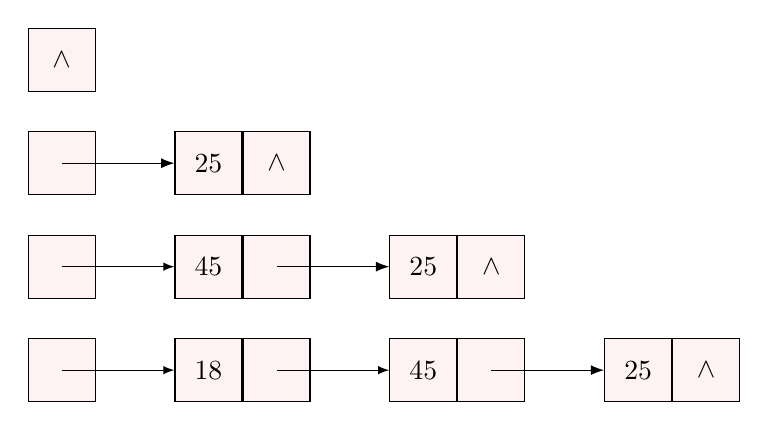
\begin{tikzpicture}[fill=red, box/.style={draw, minimum width=0.85cm, minimum height=0.8cm, fill=red!5}]
	          \draw node[box] (h) {$\wedge$};

	          \draw node[box, below=0.5 of h] (h) {} node[box, right=of h] (d25) {25}  node[box, right=0 of d25] (p25) {$\wedge$};
	          \draw[draw, -Latex] (h.center) -- (d25);

	          \draw node[box, below=0.5 of h] (h) {}
            node[box, right=of h] (d45) {45}  node[box, right=0 of d45] (p45) {}
            node[box, right=of p45] (d25) {25}  node[box, right=0 of d25] (p25) {$\wedge$};
	          \draw[draw, -Latex] (h.center)  edge[-latex] (d45) (p45.center) -- (d25);

	          \draw node[box, below=0.5 of h] (h) {}
            node[box, right=of h] (d18) {18}  node[box, right=0 of d18] (p18) {}
            node[box, right=of p18] (d45) {45}  node[box, right=0 of d45] (p45) {}
            node[box, right=of p45] (d25) {25}  node[box, right=0 of d25] (p25) {$\wedge$};
	          \path[draw, -Latex] (h.center) edge[-latex] (d18) (p18.center)  edge[-latex] (d45)  (p45.center) -- (d25);
          \end{tikzpicture}
        }
      \end{tcolorbox}

    \end{column}
    \begin{column}[T]{.5\linewidth}
      尾部插入:

      \begin{tcolorbox}[]
        \scalebox{0.5}{
          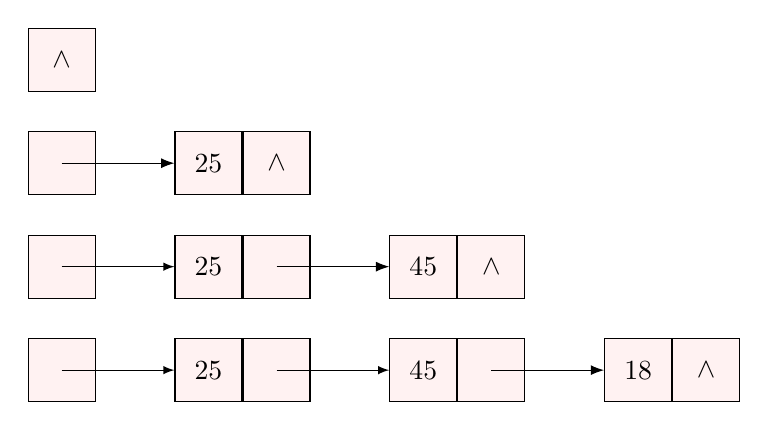
\begin{tikzpicture}[fill=red, box/.style={draw, minimum width=0.85cm, minimum height=0.8cm, fill=red!5}]
	          \draw node[box] (h) {$\wedge$};

	          \draw node[box, below=0.5 of h] (h) {} node[box, right=of h] (d25) {25}  node[box, right=0 of d25] (p25) {$\wedge$};
	          \draw[draw, -Latex] (h.center) -- (d25);

	          \draw node[box, below=0.5 of h] (h) {}
            node[box, right=of h] (d45) {25}  node[box, right=0 of d45] (p45) {}
            node[box, right=of p45] (d25) {45}  node[box, right=0 of d25] (p25) {$\wedge$};
	          \draw[draw, -Latex] (h.center)  edge[-latex] (d45) (p45.center) -- (d25);

	          \draw node[box, below=0.5 of h] (h) {}
            node[box, right=of h] (d18) {25}  node[box, right=0 of d18] (p18) {}
            node[box, right=of p18] (d45) {45}  node[box, right=0 of d45] (p45) {}
            node[box, right=of p45] (d25) {18}  node[box, right=0 of d25] (p25) {$\wedge$};
	          \path[draw, -Latex] (h.center) edge[-latex] (d18) (p18.center)  edge[-latex] (d45)  (p45.center) -- (d25);
          \end{tikzpicture}
        }
      \end{tcolorbox}

    \end{column}
  \end{columns}
\end{frame}

\begin{frame}[fragile]
  \frametitle{建立单链表:头部插入}

  \begin{center}
    \begin{tcolorbox}[]
        \scalebox{0.5}{
          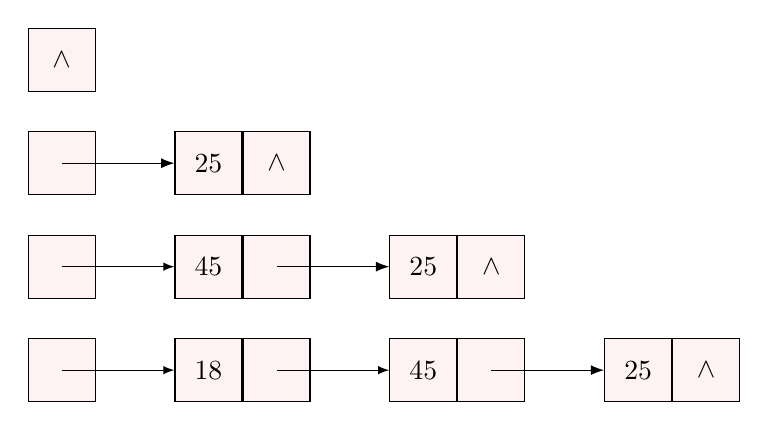
\begin{tikzpicture}[fill=red, box/.style={draw, minimum width=0.85cm, minimum height=0.8cm, fill=red!5}]
	          \draw node[box] (h) {$\wedge$};

	          \draw node[box, below=0.5 of h] (h) {} node[box, right=of h] (d25) {25}  node[box, right=0 of d25] (p25) {$\wedge$};
	          \draw[draw, -Latex] (h.center) -- (d25);

	          \draw node[box, below=0.5 of h] (h) {}
            node[box, right=of h] (d45) {45}  node[box, right=0 of d45] (p45) {}
            node[box, right=of p45] (d25) {25}  node[box, right=0 of d25] (p25) {$\wedge$};
	          \draw[draw, -Latex] (h.center)  edge[-latex] (d45) (p45.center) -- (d25);

	          \draw node[box, below=0.5 of h] (h) {}
            node[box, right=of h] (d18) {18}  node[box, right=0 of d18] (p18) {}
            node[box, right=of p18] (d45) {45}  node[box, right=0 of d45] (p45) {}
            node[box, right=of p45] (d25) {25}  node[box, right=0 of d25] (p25) {$\wedge$};
	          \path[draw, -Latex] (h.center) edge[-latex] (d18) (p18.center)  edge[-latex] (d45)  (p45.center) -- (d25);
          \end{tikzpicture}
        }
      \end{tcolorbox}

  \end{center}

  \begin{minted}[]{java}
Node s = new Node(val);//s指向新结点
s.next = head;//新结点后继为当前头结点
head = s;//头指针指向新结点
  \end{minted}

  \pause
  \color{red} 在空表时是否可行?
\end{frame}


\begin{frame}[fragile]
  \frametitle{建立单链表:尾部插入}

  \begin{center}
    \begin{tcolorbox}[]
        \scalebox{0.5}{
          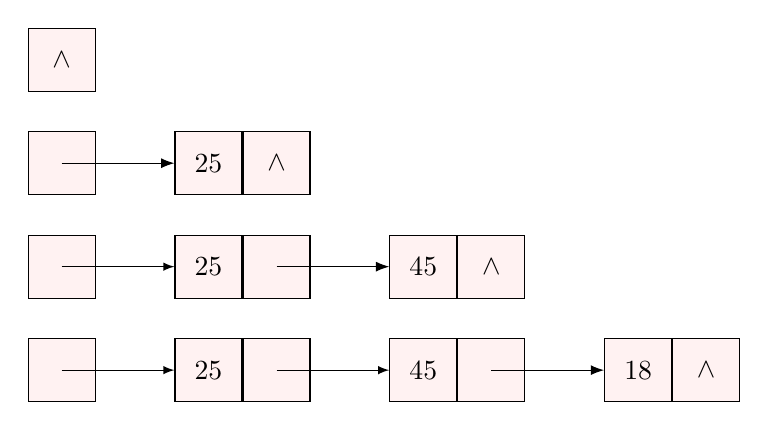
\begin{tikzpicture}[fill=red, box/.style={draw, minimum width=0.85cm, minimum height=0.8cm, fill=red!5}]
	          \draw node[box] (h) {$\wedge$};

	          \draw node[box, below=0.5 of h] (h) {} node[box, right=of h] (d25) {25}  node[box, right=0 of d25] (p25) {$\wedge$};
	          \draw[draw, -Latex] (h.center) -- (d25);

	          \draw node[box, below=0.5 of h] (h) {}
            node[box, right=of h] (d45) {25}  node[box, right=0 of d45] (p45) {}
            node[box, right=of p45] (d25) {45}  node[box, right=0 of d25] (p25) {$\wedge$};
	          \draw[draw, -Latex] (h.center)  edge[-latex] (d45) (p45.center) -- (d25);

	          \draw node[box, below=0.5 of h] (h) {}
            node[box, right=of h] (d18) {25}  node[box, right=0 of d18] (p18) {}
            node[box, right=of p18] (d45) {45}  node[box, right=0 of d45] (p45) {}
            node[box, right=of p45] (d25) {18}  node[box, right=0 of d25] (p25) {$\wedge$};
	          \path[draw, -Latex] (h.center) edge[-latex] (d18) (p18.center)  edge[-latex] (d45)  (p45.center) -- (d25);
          \end{tikzpicture}
        }
      \end{tcolorbox}

  \end{center}

  \begin{minted}[]{java}
Node s=new Node(val);//s指向新结点
Node r=Findlast(Head);//找到尾结点
r.next=s;//新结点成为尾结点的后继
r=s;
  \end{minted}

  \pause
  \color{red} 在空表时是否可行?
\end{frame}


\begin{frame}[fragile]
  \frametitle{建立单链表:尾部插入}
  \begin{center}
    \begin{tcolorbox}[]
        \scalebox{0.5}{
          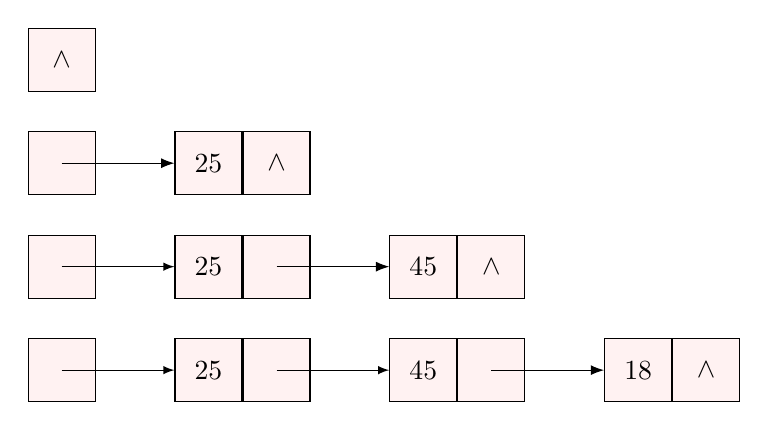
\begin{tikzpicture}[fill=red, box/.style={draw, minimum width=0.85cm, minimum height=0.8cm, fill=red!5}]
	          \draw node[box] (h) {$\wedge$};

	          \draw node[box, below=0.5 of h] (h) {} node[box, right=of h] (d25) {25}  node[box, right=0 of d25] (p25) {$\wedge$};
	          \draw[draw, -Latex] (h.center) -- (d25);

	          \draw node[box, below=0.5 of h] (h) {}
            node[box, right=of h] (d45) {25}  node[box, right=0 of d45] (p45) {}
            node[box, right=of p45] (d25) {45}  node[box, right=0 of d25] (p25) {$\wedge$};
	          \draw[draw, -Latex] (h.center)  edge[-latex] (d45) (p45.center) -- (d25);

	          \draw node[box, below=0.5 of h] (h) {}
            node[box, right=of h] (d18) {25}  node[box, right=0 of d18] (p18) {}
            node[box, right=of p18] (d45) {45}  node[box, right=0 of d45] (p45) {}
            node[box, right=of p45] (d25) {18}  node[box, right=0 of d25] (p25) {$\wedge$};
	          \path[draw, -Latex] (h.center) edge[-latex] (d18) (p18.center)  edge[-latex] (d45)  (p45.center) -- (d25);
          \end{tikzpicture}
        }
      \end{tcolorbox}

  \end{center}

  \begin{minted}[]{java}
Node s=new Node(val);
if(!head)  // 空表,插入第一个结点
    head=s; //新结点作为第一个结点
else // 非空表
    r.next=s;//新结点作为最后一个结点的后继

r=s; // 尾指针r 指向新的尾结点
  \end{minted}
\end{frame}

\begin{frame}[fragile]
  \frametitle{头结点问题}
  \begin{easylist}
    & 在上面的算法中,空表和非空表的处理是不同的

    && 当链表为空,新结点作为第一个结点,地址放在链表头指针变量中(第一个结点没
      有前驱,其地址就是整个链表的地址);

    && 否则,新结点地址放在其前驱的指针域。

    & 上述问题在很多操作中都会遇到,为方便操作,可在链表头部加一个“头结点”。
  \end{easylist}

\end{frame}

\begin{frame}[fragile]
  \frametitle{头结点问题}
  \begin{easylist}
    & 头结点的类型与数据结点一致,其数据域无定义,指针域中存放的是第一个数据结点
    的地址,空表时为空。头结点的数据域可以为空,也可存放线性表长度等附加信息,但
    此结点不能计入链表长度值。

    & 加入头结点完全是为了运算的方便。有了头结点,即使是空表,头指针变量head(或
      记作h,或者hp: head pointer)也不为空,空表和“非空表”的处理成为一致。

    & 注意区分:头节点和指向头节点的指针
  \end{easylist}

  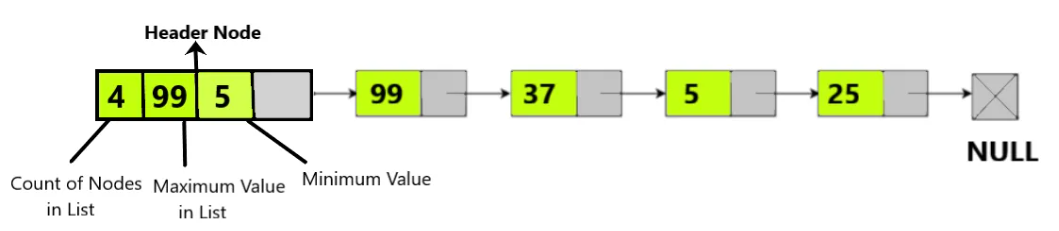
\includegraphics[width=0.8\textwidth]{figs/list/header_node_1.png}
\end{frame}

\begin{frame}[fragile]
  \frametitle{求表长}
  \begin{center}
    \scalebox{0.65}{
      \begin{tikzpicture}[fill=red, box/.style={draw, minimum width=0.85cm, minimum height=0.8cm, fill=red!5}]
	      \draw node[box, dashed] (h) {$hp$}
        node[box, thick, double, pattern=north west lines, right=of h] (d18) { }  node[box, thick, double, right=0 of d18] (p18) {}
        node[box, right=of p18] (d45) {45}  node[box, right=0 of d45] (p45) {}
        node[box, right=of p45] (d25) {25}  node[box, right=0 of d25] (p25) {$\wedge$}
	      node[below=1 of h] (tip1) {指向头节点的指针} node[below=1.5 of p18] (tip2) {头节点};
	      \path[draw, -Latex] (h) edge[-latex] (d18) (p18.center)  edge[-latex] (d45)  (p45.center) -- (d25);
	      \path (tip1) edge[draw=red,  thick, ->, out=45, in=270] (h) (tip2) edge[draw=red, thick, in=270, ->] (d18);
      \end{tikzpicture}
    }
  \end{center}

  \scriptsize
  \begin{columns}
    \begin{column}[T]{0.5\linewidth}
      \begin{minted}{c}
        int GetLength() {
          Node p= hp.next; // hp: head pointer
          int  len=0;
          while (p){
            p=p.next;
            len++;
          }
          return  len;
        }
      \end{minted}
    \end{column}
    \begin{column}[T]{0.5\linewidth}
      \pause
      \begin{minted}{python}
class Node:
    def __init__(self, data, next=None):
        self.data = data
        self.next = next

def get_length(hp):
    p = hp.next
    len = 0
    while(p!=None):
        p = p.next
        len = len + 1
    return len

hp = Node(None, Node(45, Node(25)))
print(get_length(hp))
      \end{minted}
    \end{column}
  \end{columns}
\end{frame}

\begin{frame}[fragile]
  \frametitle{单链表的查找}
  \begin{center}
    \scalebox{0.65}{
      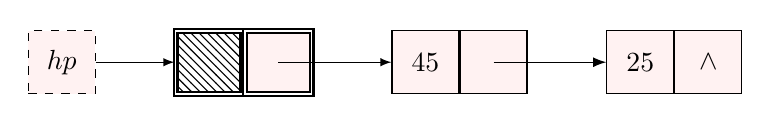
\begin{tikzpicture}[fill=red, box/.style={draw, minimum width=0.85cm, minimum height=0.8cm, fill=red!5}]
	      \draw node[box, dashed] (h) {$hp$}
        node[box, thick, double, pattern=north west lines, right=of h] (d18) { }  node[box, thick, double, right=0 of d18] (p18) {}
        node[box, right=of p18] (d45) {45}  node[box, right=0 of d45] (p45) {}
        node[box, right=of p45] (d25) {25}  node[box, right=0 of d25] (p25) {$\wedge$};
	      \path[draw, -Latex] (h) edge[-latex] (d18) (p18.center)  edge[-latex] (d45)  (p45.center) -- (d25);
      \end{tikzpicture}
    }
  \end{center}

  \begin{itemize}
  \item 按值查找index(value): 是否存在数据元素X?序号是?
  \item 算法思路:“顺藤摸瓜”——从第一个结点开始,判断当前结点的值是否等于x,若是
    则返回该结点的指针,否则继续检查下一个,直到表尾。如果找不到则返回空。
  \end{itemize}

  \begin{minted}{c}
public int index(value){   //在L中查找值为x的结点
  Node  p=hp.next;  int j=0;
  while ( p && p.data !=value){
    p=p->next; j++;
  }
  if(p) return j; else return -1;
}
  \end{minted}
\end{frame}

\begin{frame}[fragile]
  \frametitle{插入新结点:在给定结点的前后}
  \begin{itemize}
  \item 新结点插入到p的后面
    \scalebox{0.65}{
      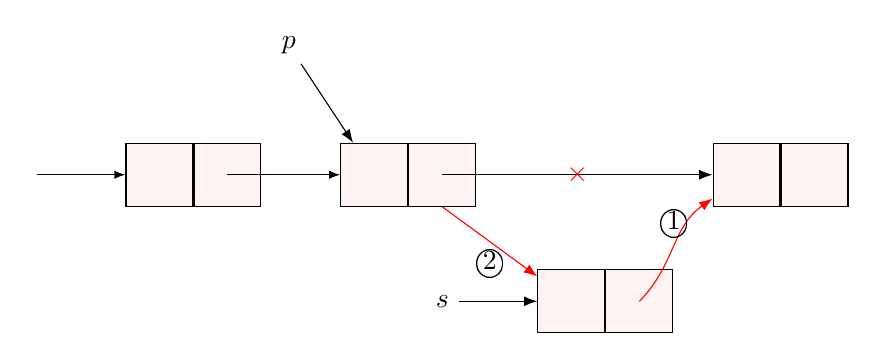
\begin{tikzpicture}[fill=red, box/.style={draw, minimum width=0.85cm, minimum height=0.8cm, fill=red!5}]
        \draw node[] (h) {}
        node[box, right=of h] (d1) { }  node[box, right=0 of d1] (p1) { ~ }
        node[box, right=of p1] (d2) {}  node[box, right=0 of d2] (p2) { ~ }
        node[box, right=3cm of p2] (d3) {}  node[box, right=0 of d3] (p3) {};

        \path[] (h.center) edge[-latex] (d1) (p1.center) edge[-latex] (d2) (p2.center) edge[draw, -Latex] node[color=red] {$\times$} (d3);

        \draw node[above right=of d1](p) {$p$};
        \draw[draw, -Latex] (p) --(d2);

        \draw node[below=of p2] (s) {$s$}
        node[box, right=of s] (ds) { }  node[box, right=0 of ds] (ps) { ~ };
        \draw[draw, -Latex] (s) --(ds);

        \path[] (p2.south) edge[draw=red, -Latex] node[below, align=center] {\textcircled{2}} (ds);
        \path[] (ps.center) edge[draw=red, -Latex, in=215] node[above, align=center] {\textcircled{1}} (d3);
      \end{tikzpicture}
    }

    \begin{minted}{c}
      s.next = p.next;
      p.next = s;
    \end{minted}

  \end{itemize}
\end{frame}

\begin{frame}[fragile]
  \frametitle{插入新结点:在给定结点的前后}
  \begin{itemize}
  \item 新结点插入到p的前面
    \scalebox{0.65}{
      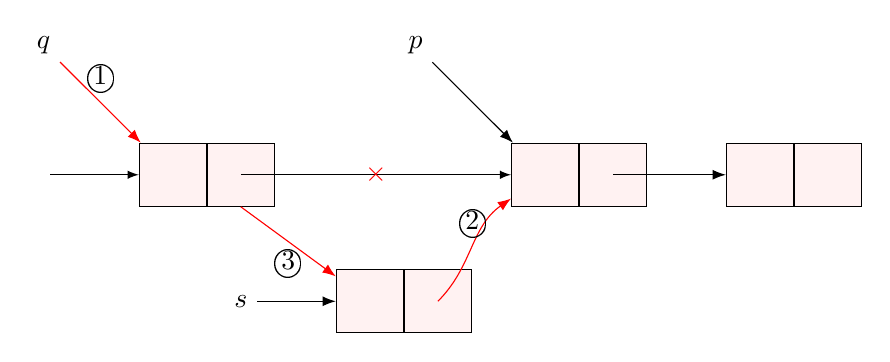
\begin{tikzpicture}[fill=red, box/.style={draw, minimum width=0.85cm, minimum height=0.8cm, fill=red!5}]
        \draw node[] (h) {}
        node[box, right=of h] (d1) { }  node[box, right=0 of d1] (p1) { ~ }
        node[box, right=3cm of p1] (d2) {}  node[box, right=0 of d2] (p2) { ~ }
        node[box, right=of p2] (d3) {}  node[box, right=0 of d3] (p3) {};

        \path[] (h.center) edge[-latex] (d1) (p1.center) edge[-latex] node[color=red] {$\times$} (d2) (p2.center) edge[draw, -Latex]  (d3);

        \draw node[above left=of d2](p) {$p$};
        \draw[draw, -Latex] (p) --(d2);

        \draw node[above left=of d1](q) {$q$};
        \path (q)  edge[draw=red, -Latex] node[above] {\textcircled{1}} (d1);

        \draw node[below=of p1] (s) {$s$}
        node[box, right=of s] (ds) { }  node[box, right=0 of ds] (ps) { ~ };
        \draw[draw, -Latex] (s) --(ds);

        \path[] (p1.south) edge[draw=red, -Latex] node[below, align=center] {\textcircled{3}} (ds);
        \path[] (ps.center) edge[draw=red, -Latex, in=215] node[above, align=center] {\textcircled{2}} (d2);
      \end{tikzpicture}
    }

    找到p的前驱q,在q之后插入s。

    \begin{minted}{c}
q=head;
while (q.next!=p) q=q.next;
s.next=q.next;
q.next=s;
    \end{minted}
  \end{itemize}
\end{frame}

\begin{frame}[fragile]
  \frametitle{插入新结点}
  \begin{easylist}
    & 时间复杂度
    && 后插操作为$O(1)$: 不受$n$的影响
    && 前插操作因为要先找到$p$的前驱,时间性能为$O(n)$。

    \pause
    & 一个小技巧:
    && 将$s$插入到 $p$ 的后面,然后把$p.data$与$s.data$交换,这样能使得时间复杂性为$O(1)$。
  \end{easylist}
\end{frame}

\begin{frame}[fragile]
  \frametitle{删除结点}
  \begin{itemize}
  \item 删除p指向的结点 \\

    \scalebox{0.6}{
      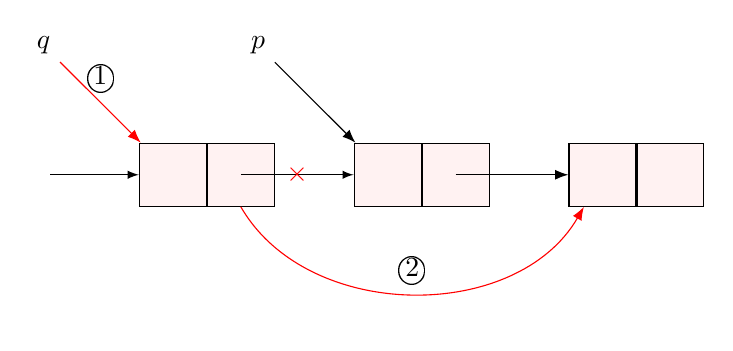
\begin{tikzpicture}[fill=red, box/.style={draw, minimum width=0.85cm, minimum height=0.8cm, fill=red!5}]
        \draw node[] (h) {}
        node[box, right=of h] (d1) { }  node[box, right=0 of d1] (p1) { ~ }
        node[box, right=of p1] (d2) {}  node[box, right=0 of d2] (p2) { ~ }
        node[box, right=of p2] (d3) {}  node[box, right=0 of d3] (p3) {};

        \path[] (h.center) edge[-latex] (d1) (p1.center) edge[-latex] node[color=red] {$\times$} (d2) (p2.center) edge[draw, -Latex]  (d3);

        \draw node[above left=of d2](p) {$p$};
        \draw[draw, -Latex] (p) --(d2);

        \draw node[above left=of d1](q) {$q$};
        \path (q)  edge[draw=red, -Latex] node[above] {\textcircled{1}} (d1);

        \path (p1.south)  edge[draw=red, -Latex, in=240, out=300] node[above]{\textcircled{2}} (d3);
      \end{tikzpicture}
    }

    q.next=q.next.next;
  \item 首先要找到$p$的前驱结点$q$,其时间复杂性为$O(n)$。

  \item 若要删除$p$的后继结点(假设存在),则可以直接完成:\\
    p.next=p.next.next;
  \item 该操作的时间复杂性为$O(1)$ 。
  \end{itemize}
\end{frame}

\begin{frame}[fragile]
  \frametitle{删除第i个结点}
  \begin{minted}{c}
    int  Del(LinkList  L, int i)  //删除链表L第i个结点
    {
      p=get(L, i-1);  //查找第i-1个结点
      if (p==NULL) {
        printf("第i-1个结点不存在");   return -1;
      } else{
        if (!p->next)
          return 0; //第i个结点不存在
        else {
          p.next=p.next.next; //从链表中删除i
          return 1;
        }
      }
    }
  \end{minted}

  算法时间复杂度是$O(n)$
\end{frame}

\begin{frame}[fragile]
  \frametitle{单链表操作小结}
  \begin{itemize}
  \item 在单链表上当前结点之前插入、删除一个结点,必须知道其前驱结点。
  \item 单链表不具有按序号随机访问的特点,只能从头指针开始一个个顺序进行。
  \end{itemize}
\end{frame}

\begin{frame}[fragile]
  \frametitle{单循环链表}
  \begin{easylist}
    & 链表头尾结点相连

    \begin{center}
      \scalebox{0.65}{
        \begin{tikzpicture}[fill=red, box/.style={draw, minimum width=0.85cm, minimum height=0.8cm, fill=red!5}]
	        \draw node[box, dashed] (hp) {$hp$}
          node[box, thick, double, pattern=north west lines, right=of hp] (dh) { }  node[box, thick, double, right=0 of dh] (ph) {}
          node[box, right=of ph] (da1) {$a_1$}  node[box, right=0 of da1] (pa1) {}
          node[box, draw=none, right=of pa1] (dai) {$\cdots$}  node[box, draw=none,  right=0 of dai] (pai) {$\cdots$}
          node[box, right=of pai] (dan) {$a_n$}  node[box, right=0 of dan] (pan) {};

	        \path[draw, -Latex] (hp) edge[-latex] (dh) (ph.center)  edge[-Latex] (da1)
			    (pa1.center) edge[-Latex] (dai)
			    (pai.east) edge[-Latex] (dan)
			    (pan.center)  |- ++(0,-1) -| (dh);

          \draw node[box, dashed, right=1cm of pan] (hp) {$hp$}
          node[box, thick, double, pattern=north west lines, right=of hp] (dh) { }  node[box, thick, double, right=0 of dh] (ph) {};

          \path[draw, -Latex] (hp) edge[-latex] (dh) (ph.center)
			    (ph.center)  |- ++(0,-1) -| (dh);

          \draw node[below=1cm of pa1] {(a) 非空表} node[below=1cm of dh] {(b) 空表};
        \end{tikzpicture}
      }
    \end{center}

    & 结点的定义有什么变化?

    & 链表操作有什么变化?比如:

    && 原来用头结点的next是否为NULL (None)判断空表,现在呢?

    && 原来用结点的next是否为NULL (None)判断尾结点,现在呢?
  \end{easylist}
\end{frame}

\begin{frame}[fragile]
  \frametitle{双向链表}

  \begin{center}
    \scalebox{0.5}{
      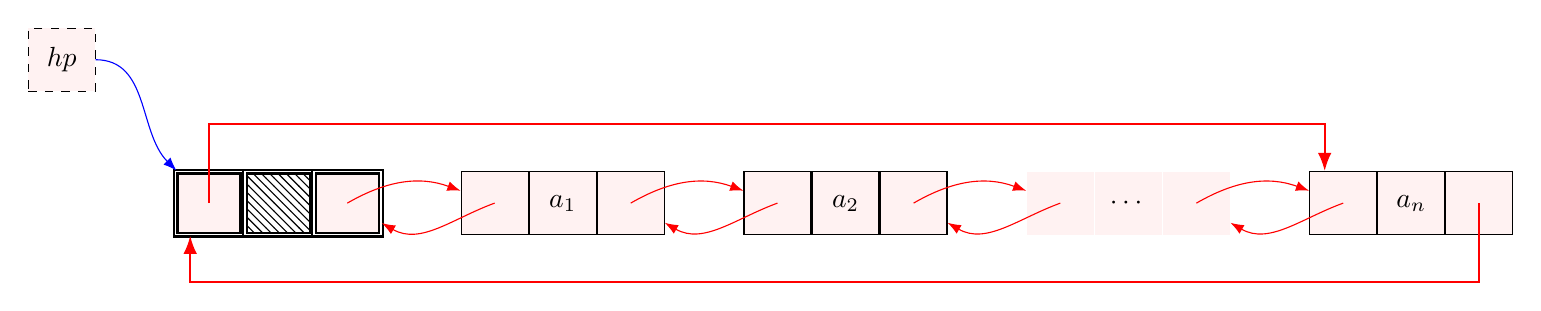
\begin{tikzpicture}[fill=red, box/.style={draw, minimum width=0.85cm, minimum height=0.8cm, fill=red!5},
          e1/.style={draw=red, -Latex, in=160, out=30},
          e2/.style={draw=red, -Latex, in=-30, out=200}
        ]
	      \draw node[box, dashed] (hp) {$hp$}
		    node[box, thick, double,below right=of hp] (prevh) { }
        node[box, thick, double, pattern=north west lines, right=0 of prevh] (datah) { }  node[box, thick, double, right=0 of datah] (nexth) {}

		    node[box, right=of nexth] (prev1) {}   node[box, right=0 of prev1] (data1) {$a_1$}  node[box, right=0 of data1] (next1) {}

		    node[box, right=of next1] (prev2) {}   node[box, right=0 of prev2] (data2) {$a_2$}  node[box, right=0 of data2] (next2) {}

		    node[box, right=of next2, draw=none] (previ) {}   node[box, right=0 of previ, draw=none] (datai) {$\cdots$}  node[box, right=0 of datai, draw=none] (nexti) {}

		    node[box, right=of nexti] (prevn) {}   node[box, right=0 of prevn] (datan) {$a_n$}  node[box, right=0 of datan] (nextn) {};

        \path (hp) edge[out=0, -Latex, draw=blue] (prevh)
	      (nexth.center) edge[e1] (prev1)
        (next1.center) edge[e1] (prev2)
        (next2.center) edge[e1] (previ)
        (nexti.center) edge[e1] (prevn)
	      (prev1.center) edge[e2] (nexth)
        (prev2.center) edge[e2] (next1)
        (previ.center) edge[e2] (next2)
        (prevn.center) edge[e2] (nexti);

        \path[draw=red, thick, -Latex]  (nextn.center)  |- ++(0,-1) -| (prevh.240);
        \path[draw=red, thick, -Latex]  (prevh.center)  |- ++(0,1) -| (prevn.120);
      \end{tikzpicture}
    }

    \scriptsize (a) 有多个节点时的双向链表
  \end{center}

  \begin{columns}
    \begin{column}[T]{0.65\linewidth}
      \scriptsize
      \begin{itemize}
      \item 为什么需要双向链表?
      \item 在单链表中查找后继的时间性能是$O(1)$,查找前驱的时间性能是$O(n)$,如果也
        希望找前驱的时间性能达到$O(1)$,则需要在空间上付出代价 —— 每个结点再加一个指
        向前驱的指针域。
      \item 结点的定义和链表的操作有什么变化?

        \begin{minted}{java}
          class Node {
            Object data;
            Node prior, next;
          }
        \end{minted}
      \end{itemize}
    \end{column}
    \begin{column}[T]{0.35\linewidth}
      \begin{center}
        \scalebox{0.5}{
          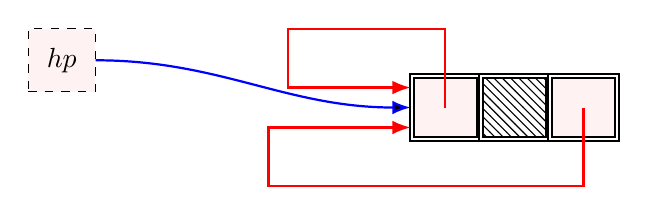
\begin{tikzpicture}[fill=red, box/.style={draw, minimum width=0.85cm, minimum height=0.8cm, fill=red!5},
              e1/.style={draw=red, -Latex, in=160, out=30},
              e2/.style={draw=red, -Latex, in=-30, out=200}
            ]
	          \draw node[box, dashed] (hp) {$hp$}
		        node[box, thick, double, right=4cm of hp, yshift=-0.6cm] (prevh) { }
            node[box, thick, double, pattern=north west lines, right=0 of prevh] (datah) { }  node[box, thick, double, right=0 of datah] (nexth) {};

            \path[draw=blue, thick, -Latex]  (hp)  edge[out=0, in=180] (prevh.180);
            \path[draw=red, thick, -Latex]  (nexth.center)  |- ++(0,-1) -- ++(-4,0) |- (prevh.210);
            \path[draw=red, thick, -Latex]  (prevh.center)  |- ++(0,1) -- ++(-2,0)  |- (prevh.150);
          \end{tikzpicture}
        }

      \scriptsize (b) 只有头节点的情况
      \end{center}
    \end{column}
  \end{columns}
\end{frame}

\begin{frame}[fragile]
  \frametitle{链表特点}
  \begin{center}
    \scalebox{0.65}{
      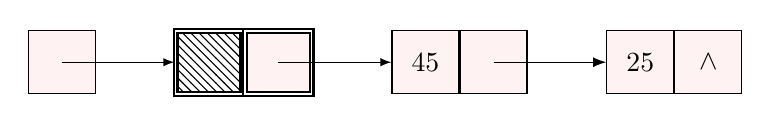
\begin{tikzpicture}[fill=red, box/.style={draw, minimum width=0.85cm, minimum height=0.8cm, fill=red!5}]
	      \draw node[box] (h) {}
        node[box, thick, double, pattern=north west lines, right=of h] (d18) { }  node[box, thick, double, right=0 of d18] (p18) {}
        node[box, right=of p18] (d45) {45}  node[box, right=0 of d45] (p45) {}
        node[box, right=of p45] (d25) {25}  node[box, right=0 of d25] (p25) {$\wedge$};
	      \path[draw, -Latex] (h.center) edge[-latex] (d18) (p18.center)  edge[-latex] (d45)  (p45.center) -- (d25);
      \end{tikzpicture}
    }
  \end{center}

  \begin{easylist}
    & 优点

    && 插入删除方便

    && 动态分配

    \pause

    & 缺点

    && 随机访问效率低
  \end{easylist}
\end{frame}

\begin{frame}[fragile]
  \frametitle{顺序表 VS 链表}
  \begin{columns}
    \begin{column}[T]{0.5\linewidth}
      \begin{tcolorbox}[colframe=red, title=顺序表优点]
        \begin{itemize}
        \item 直观
        \item 随机访问效率高
        \item 没有为表达结点间的逻辑关系增加的额外开销
        \end{itemize}
      \end{tcolorbox}

      \begin{tcolorbox}[colframe=red, title=顺序表缺点]
        \begin{itemize}
        \item 插入删除时效率低
        \item 需要预先分配足够大的存储空间
        \end{itemize}
      \end{tcolorbox}
    \end{column}
    \begin{column}[T]{0.5\linewidth}
\begin{tcolorbox}[colframe=red, title=链表优点]
        \begin{itemize}
        \item 插入删除方便
        \item 动态分配
        \end{itemize}
      \end{tcolorbox}

      \begin{tcolorbox}[colframe=red, title=链表缺点]
        \begin{itemize}
        \item 为表达结点间的逻辑关系增加“指针域”
        \item 随机访问效率低
        \end{itemize}
      \end{tcolorbox}
    \end{column}
  \end{columns}
\end{frame}

\begin{frame}[fragile, allowframebreaks]
  \frametitle{选取恰当的存储结构}
  \begin{enumerate}
  \item 基于存储的考虑

    \begin{itemize}
    \item 使用顺序表,在程序执行之前要明确规定它的存储规模(对MAXSIZE要有合适的
      设定),过大造成浪费,过小造成溢出。可见对线性表的长度或存储规模难以估计时,
      不宜采用顺序表。
    \item 链表不用事先估计存储规模,但链表的存储密度较低。存储密度是指一个结点中
      数据元素所占的存储单元和整个结点所占的存储单元之比。显然链式存储结构的存储
      密度是小于1的。
    \end{itemize}

   \newpage

 \item 基于运算的考虑
   \begin{itemize}
   \item 在顺序表中按序号访问$a_i$的时间性能时$O(1)$,而链表中按序号访问的时间性
     能$O(n)$,所以如果经常做的运算是按序号访问数据元素,显然顺序表优于链表;
   \item 在顺序表中做插入、删除时平均移动表中一半的元素,如果数据元素的信息量较
     大且表较长,不可忽视这一点;
   \item 在链表中作插入、删除,虽然也要找插入位置,但操作主要是比较操作,从这个
     角度考虑优于顺序表。
   \end{itemize}

   \newpage

 \item 其它
   \begin{itemize}
   \item 顺序表容易实现,任何高级语言中都有数组类型,相对来讲简单直观,也是用户
     考虑的一个因素。
   \end{itemize}
  \end{enumerate}

  总之,两种存储结构各有长短,选择那一种由实际问题中的主要因素决定。通常“较稳定”
  的线性表选择顺序存储,而频繁做插入删除的话宜选择链式存储。
\end{frame}

\begin{frame}[fragile]
  \frametitle{本堂小结}
  \begin{enumerate}
  \item 线性表的概念和两种存储方式.
  \item 顺序线性表的特征、基本操作.
  \item 链表的特征、基本操作.
  \item 循环链表和双向链表
  \item 顺序表与链表大PK
  \item 顺序表和链表适用的场合
  \end{enumerate}
\end{frame}

\subsection{作业}
\begin{frame}[fragile]
  \frametitle{约瑟夫环}

  在罗马人占领乔塔帕特后,约瑟夫(Joseph)及他的40个战友躲到一个洞中,这些犹太人
  宁死也不想被敌人抓到,于是决定了一个自杀方式:

  \begin{itemize}
    \item 41个人排成一个圆圈,由第1个人开始报数,每报数到第3人该人就必须自杀,然
      后再由下一个重新报数,直到所有人都自杀身亡为止。
  \item 约瑟夫说他和另一个人逃过了这场死亡游戏: by luck or by the hand of God.
  \item 请问约瑟夫在这个圆圈中的位置是?
  \end{itemize}
\end{frame}

\begin{frame}[fragile]
  \frametitle{约瑟夫环}

  \begin{itemize}
  \item 已知$n$个人 (以编号$1, 2, 3 \cdots n$ 分别表示) 围坐在一张圆桌周围。从
    编号为$k$ 的人开始报数,数到$m$的那个人出列;他的下一个人又从1 开始报数,数
    到$m$的那个人又出列;依此规律重复下去,直到圆桌周围的人全部出列。

  \item 例如:n = 9, k = 1, m = 5;出局顺序如下

  \end{itemize}
  \begin{center}
    \scalebox{0.6} {
      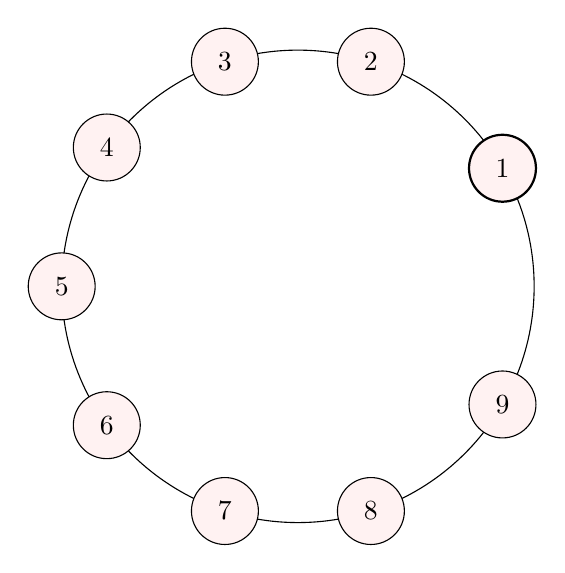
\begin{tikzpicture}[fill=red, ns/.style={draw, circle, minimum width=0.85cm, minimum height=0.8cm, fill=red!5}]
	      \node [draw, minimum size=6cm, circle] {};
        \node (n1) at (30:3cm) [ns, thick]   {1};
        \node (n2) at (72:3cm) [ns]   {2};
        \node (n3) at (108:3cm) [ns]   {3};
        \node (n4) at (144:3cm) [ns]   {4};
        \node (n5) at (180:3cm) [ns]   {5};
        \node (n6) at (216:3cm) [ns]   {6};
        \node (n7) at (252:3cm) [ns]   {7};
        \node (n8) at (288:3cm) [ns]   {8};
        \node (n9) at (330:3cm) [ns]   {9};
      \end{tikzpicture}
    }

    5, 1, 7, 4, 3, 6, 9, 2, 8
  \end{center}
\end{frame}

\begin{frame}[fragile]
  \frametitle{约瑟夫环动画演示}
  见PPT动画
\end{frame}

%\section{字符串}
\begin{frame}[fragile]
  \frametitle{字符串}
  计算机非数值处理的对象经常是字符串数据。如文本检索、文本聚类、文本理解等。

  \begin{itemize}
  \item 串的定义及表示
  \item 串的模式匹配
  \end{itemize}
\end{frame}

\begin{frame}[fragile]
  \frametitle{串 (String)的定义}

  \begin{itemize}
  \item 串是由零个或多个任意字符组成的字符序列。它也是一种特殊的线性表,其数据元
    素仅由一个字符组成,而且它通常是作为一个整体来处理。

例:s="Renmin University",s是串名, Renmin University为串值,其中一个个的字符称
为串的元素。

  \item 请思考如何实现上述串的存储?
  \end{itemize}
\end{frame}

\begin{frame}[fragile]
  \frametitle{字符串的存储}
  \begin{itemize}
  \item 顺序存储: 用一组地址连续的存储单元存储串值中的字符序列。
  \item 链式存储: 考虑到存储密度,可以按块分配。
  \item 在C++/Java等语言中,String就是字符串。在C语言中没有string类型变量,字符串用字符数组表示。
  \end{itemize}
\end{frame}

\begin{frame}[fragile]
  \frametitle{串的模式匹配}
  \begin{itemize}
  \item 设s和t是给定的两个串,在主串s中寻找等于子串t的部分的过程称为模式匹配, t也称为模式。
  \item 如果在s中找到等于t的子串,则称匹配成功,返回t在s中的首次出现的存储位置,否则匹配失败。
  \item 例:

    s="ababcabcacbab"

    t="abcac"
  \end{itemize}
\end{frame}

\begin{frame}[fragile]
  \frametitle{简单的模式匹配}
  \begin{columns}
    \begin{column}[T]{0.5\linewidth}
      s="ababcabcacbab" \\ t="abcac"

      \begin{itemize}
      \item Brute-Force算法
      \end{itemize}
    \end{column}
    \begin{column}[T]{0.5\linewidth}
      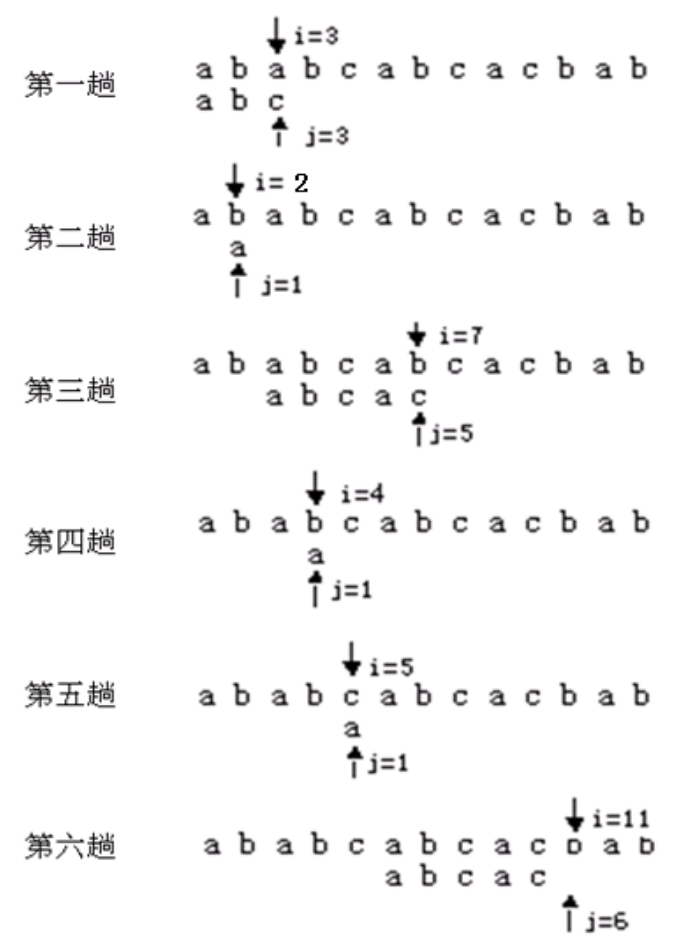
\includegraphics[width=0.9\textwidth]{figs/string/pattern-match.png}
    \end{column}
  \end{columns}
\end{frame}

\begin{frame}[fragile]
  \frametitle{BF算法时间复杂度分析}
  \begin{itemize}
  \item 设串s长度为n,串t长度为m。匹配成功的情况下,考虑两种极端情况。
    \begin{itemize}
    \item 在最好情况下,即每趟不成功的匹配都发生在第一对字符比较时。
    \item 例如:s=“aaaaaaaaaabc”,t=“bc”,设匹配成功发生在$s_i$处。
    \item 在前面i-1趟不成功的匹配中共比较了i-1次,第i趟成功的匹配共比较了m次,所
      以总共比较了i-1+m次。
    \item 所有匹配成功的可能共有n-m+1种,设从si开始与t串匹配成功的概率为$p_i$,
      在等概率情况下$p_i=1/(n-m+1)$,因此最好情况下平均比较的次数是:
      \[\sum_{i=1}^{n-m+1} p_i \times (i-1+m) = \sum_{i=1}^{n-m+1} \dfrac{1}{n-m+1} \times (i-1+m) = \dfrac{(n+m)}{2}\]

    \item 即最好情况下的时间复杂度是$O(n+m)$
    \end{itemize}
  \end{itemize}
\end{frame}

\begin{frame}[fragile]
  \begin{itemize}
  \item 在最坏情况下,即每趟不成功的匹配都发生在t的最后一个字符。
  \item 例如:s=“aaaaaaaaaaab”,t=“aaab”,设匹配成功发生在$s_i$处.
  \item 在前面$i-1$趟匹配中共比较了$(i-1) \times m$次,第$i$趟成功的匹配共比较了
    $m$次,所以总共比较了$i \times m$次,因此最坏的情况下平均比较的次数是:
    \[\sum_{i=1}^{n-m+1} p_i \times (i \times m) = \sum_{i=1}^{n-m+1} \dfrac{1}{n-m+1} \times (i \times m) = \dfrac{m \times (n-m+2)}{2}\]
  \item 即最坏情况下的时间复杂度是$O(n×m)$
  \end{itemize}

  \begin{tcolorbox}[title=为什么BF算法时间性能低?]
    在每趟匹配不成功时存在大量回溯 (每次移动一位开始新的比较)
  \end{tcolorbox}
\end{frame}

\begin{frame}[fragile]
  \frametitle{改进算法}

  \begin{tikzpicture}[box/.style={draw, minimum width=1cm, minimum height=0.8cm}]
    \draw node[minimum width=2cm] (a0) {主串};
    \foreach \i in {1,...,7} {
      \pgfmathtruncatemacro{\x}{\i - 1};
      \draw node[box, right=0 of a\x] (a\i) {A} ;
    }

		\draw node[box, right=0 of a7] (a8) {B}  node[box, right=0 of a8] (a9) {A}  node[box, right=0 of a9] (a10) {A} ;

		\draw node[below=of a0] (b0) {子串}
		node[box, below=of a1] (b1) {A}
		node[box, below=of a2] (b2) {A}
		node[box, below=of a3] (b3) {A}
		node[box, below=of a4, fill=red!50] (b4) {B} ;

	  \draw[draw=red, very thick, <-] (a4) -- ++(0,1);
	  \draw[draw=red, very thick, <-] (b4) -- ++(0,-1);

    \path (a4) edge[draw=red, in=90, out=115, ->, dotted, thick]  (a2);
    \path (b4) edge[draw=red, in=-90, out=-115, ->, dotted, thick]  (b1);
  \end{tikzpicture}

  \begin{itemize}
  \item 改进算法的目的是在每一趟匹配过程中出现不匹配时,向右“滑动”尽可能远的一段
    距离后,继续进行比较。那么,应当滑动多远呢?这正是各个算法各显神通之处!

  \item KMP算法: 由D. E. Knuth,J. H. Morris和V. R. Pratt同时发现

    % \item Boyer-Moore算法
  \end{itemize}
\end{frame}

\begin{frame}[fragile]
  \frametitle{KMP算法}
  利用已经得到的“部分匹配”的结果将模式向右滑动

  视频讲解:\url{https://www.bilibili.com/video/BV1AY4y157yL/}

\end{frame}

\begin{frame}[fragile]
  \frametitle{KMP算法}
  利用ChatGPT来完成代码,已经变得非常方便,参见string.ipynb文件。

\end{frame}

\begin{frame}[fragile]
  \frametitle{练习}
  \begin{itemize}
  \item 从《红楼梦》中,统计主要人物出现的次数,并按照频次高低输出。

  \item 文件位置:ipynb/honglou.txt

  \item 人物列表:ipynb/honglou\_person.txt
  \end{itemize}
\end{frame}


\begin{frame}[fragile]
  \frametitle{多模式串匹配与AC自动机}
    \begin{itemize}
    \item BM、KMP为单模匹配,即模式串只有一个。假设主串$T[1, \cdots, m]$,
    模式串有k个$P={P_1,\cdots,P_k}$,且模式串集合的总长度为$n$。
    如果采用KMP来匹配多模式串,则算法复杂度为:

    \[O(|P_1|+m+\cdots+|P_k|+m)=O(n+km)\]
  
    \item KMP并没有利用到模式串之间的重复字符结构信息,每一次模式串的匹配都需要将主串从头至尾扫描一遍。

    \item 贝尔实验室的Aho与Corasick于1975年基于有限状态机(finite state machines)提出AC自动机算法
  \footnote{AC算法比KMP提出要早,KMP于1977年提出}。
  \end{itemize}
  % https://www.cnblogs.com/en-heng/p/5247903.html
\end{frame}

\begin{frame}[fragile]
  \frametitle{AC自动机}
  \begin{itemize}
  \item 自动机由状态(数字标记的圆圈)和转换(带标签的箭头)组成,每一次转换对应一个字符。AC算法的核心包括三个函数:goto、failure、output;这三个函数构成了AC自动机。对于模式串{he, his, hers, she},goto函数表示字符按模式串的转移,暗含了模式串的共同前缀的字符结构信息\footnote{\url{from: https://www.cnblogs.com/en-heng/p/5247903.html}}。
  \end{itemize}

  \begin{center}
  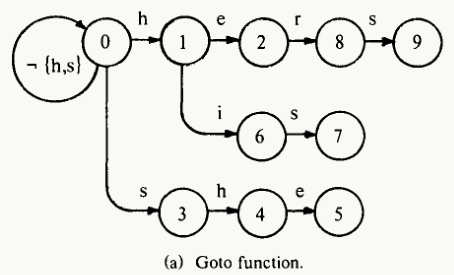
\includegraphics[width=0.55\textwidth]{figs/string/ac_goto.png}
  \end{center}
\end{frame}

\begin{frame}[fragile]
  \frametitle{AC自动机}
  \begin{itemize}
  \item failure函数表示匹配失败时退回的状态:
  \end{itemize}

  \begin{center}
  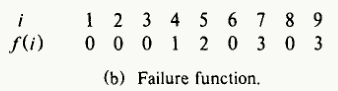
\includegraphics[width=0.6\textwidth]{figs/string/ac_failure.png}
  \end{center}
\end{frame}

\begin{frame}[fragile]
  \frametitle{AC自动机}
  \begin{itemize}
  \item output函数表示模式串对应于自动机的状态:
  \end{itemize}

  \begin{center}
  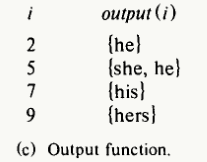
\includegraphics[width=0.4\textwidth]{figs/string/ac_output.png}
  \end{center}
\end{frame}

\begin{frame}[fragile]
  \frametitle{AC自动机}
  \begin{itemize}
  \item 完整的AC自动机如下:
  \end{itemize}

  \begin{center}
  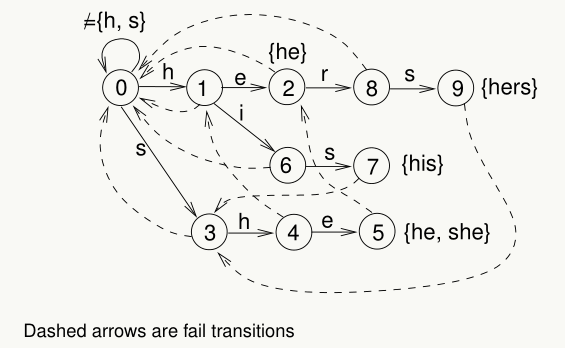
\includegraphics[width=0.8\textwidth]{figs/string/ac.png}
  \end{center}
\end{frame}

\begin{frame}[fragile]
  \frametitle{AC自动机匹配过程}
  AC算法根据自动机匹配模式串,过程比较简单:从主串的首字符、自动机的初始状态0开始,

  \begin{itemize}
  \item 若字符匹配成功,则按自动机的goto函数转移到下一状态;且若转移的状态对应有output函数,则输出已匹配上的模式串;
  \item 若字符匹配失败,则递归地按自动机的failure函数进行转移
  \end{itemize}
\end{frame}


\section{Tree}


\begin{frame}[fragile]{树和二叉树}
  \begin{columns}[T]
    \column{0.5\textwidth}

    树型结构是结点之间有分支,并且具有层次关系的结构,类似于自然界中的树。树有很多
    应用,比如Unix等操作系统中的目录结构。

    \column{0.4\textwidth}
    \includegraphics[width=0.9\textwidth]{figs/linux-tree.png}
  \end{columns}
\end{frame}

\begin{frame}[fragile]
  \frametitle{例子}
\begin{forest}
 [CEO, for tree={rectangle, minimum width=2cm}, fill=red!10
    [CFO [财务人员] ]
    [CTO [工程师] ]
    [CMO [销售人员] ]
 ]
 \node at (current bounding box.south)
 [below=1ex,draw,cloud,aspect=6,cloud puffs=30]
 {\emph{Simple Company Hierarchy}};
\end{forest}
\end{frame}

\begin{frame}[fragile, plain]
  \scalebox{0.7}{
    \begin{forest}
      [学院, for tree={draw=none, rectangle, minimum width=1cm}, fill=red!10, circle
       [社会学部, grow=west [信息资源管理学院, fill=red!10] [新闻学院] [农业与农村发展学院] [社会与人口学院]
       [公共管理学院] [教育学院]]
       [$\cdots$]
       [ 人文学部,grow=east [哲学院] [文学院] [历史学院] [国学院] [艺术学院] [外国语学院] [清史研究所]]
       ]
       \node at (current bounding box.south)
       [below=1ex,draw,cloud,aspect=6,cloud puffs=30]
       {\emph{人民大学学院设置}};
    \end{forest}
  }
\end{frame}

\begin{frame}[fragile]{内容}
  \begin{easylist} \easyitem
    & 树的基本术语
    & 二叉树
    & 遍历二叉树与线索二叉树
    & 树和森林
    & 哈夫曼树
  \end{easylist}
\end{frame}

\subsection{基本术语}

\begin{frame}[fragile]
  \frametitle{树(TREE)}树(Tree)是$n(n \geq 0)$个结点的有限集$T$。 $T$为空时称为空
  树。当$n>0$时,树有且仅有一个特定的称为根(Root)的结点,其余结点可分为$m(m \geq
  0)$个互不相交的子集$T_1, T_2, \cdots, T_m$,其中每个子集又是一棵树,称为子
  树(Subtree)。
  \begin{columns}[T]
    \column{0.55\textwidth}
    \begin{easylist}
    & 各子树是互不相交的集合。
    & 除根结点,其它结点有唯一前驱。
    & 一个结点可以有零个或多个后继。
    \end{easylist}

    \column{0.4\textwidth}
    \begin{forest}
      [R, for tree={color=white,fill=black}, fill=red!85
      [A [C] [D] [E]]
      [B [F]]
      ]
    \end{forest}
  \end{columns}
\end{frame}

\begin{frame}[fragile]
  \frametitle{判断哪些是树结构}
  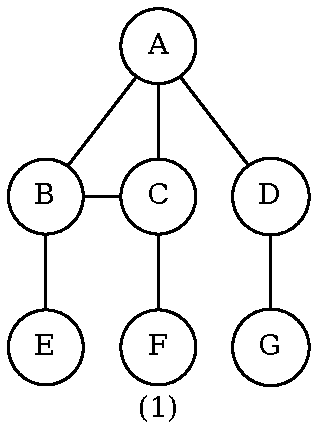
\includegraphics[width=0.3\textwidth]{dot/tree-judge1.pdf} ~~~~~
  \pause
  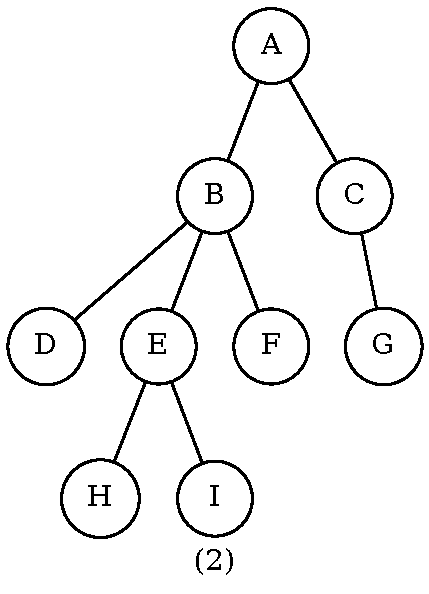
\includegraphics[width=0.4\textwidth]{dot/tree-judge2.pdf}
\end{frame}

\begin{frame}[fragile]
  \frametitle{判断哪些是树结构}
  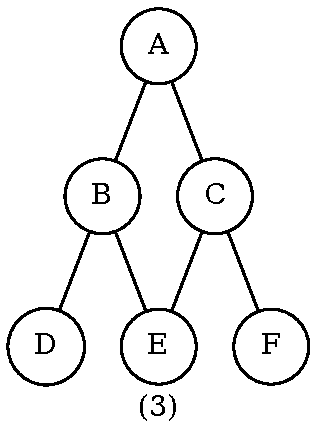
\includegraphics[width=0.35\textwidth]{dot/tree-judge3.pdf} ~~~~~
  \pause
  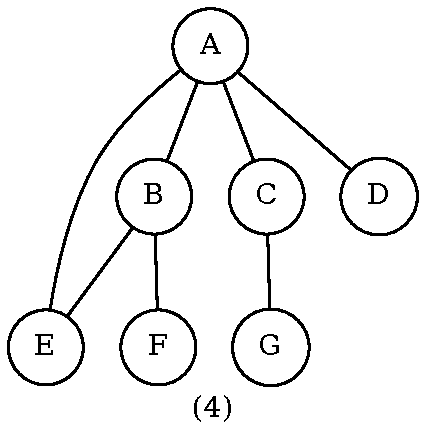
\includegraphics[width=0.4\textwidth]{dot/tree-judge4.pdf}
\end{frame}

\begin{frame}[fragile]
  \frametitle{树的表示形式}
  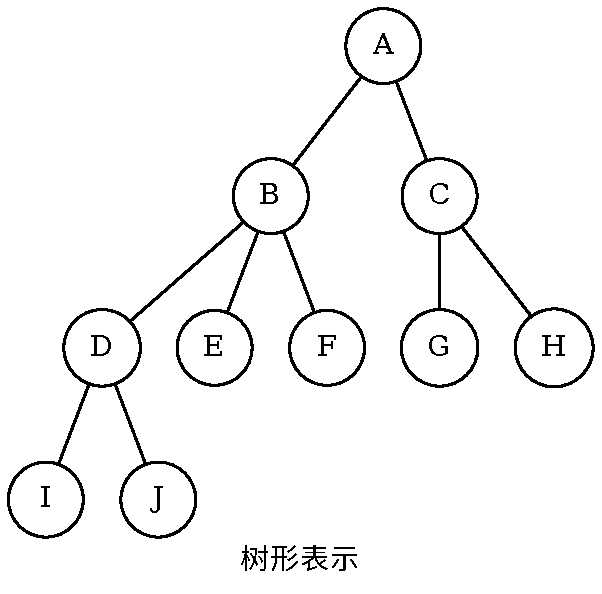
\includegraphics[width=0.36\textwidth]{dot/tree-represent1.pdf}  \pause
  \scalebox{0.75}{
    \begin{tikzpicture}[b/.style={fill=black!50},n/.style={minimum width=1cm}]
      \draw node[n] (a) {A} node[b, right=0 of a, minimum width=5cm, fill=red!50]{};  

      \draw node[minimum width=0.5cm, below=0.1 of a](bh){} 
      node[n, right=0 of bh] (b) {B} node[b,fill=blue!50, minimum width=4.3cm,right=0 of b]{};  

      \draw node[minimum width=2cm, below=0.2 of bh](dh){} 
      node[n, right=0 of dh] (d) {D} node[b, minimum width=3.5cm,right=0 of d]{}; 

      \draw node[minimum width=3.5cm, below=0.2 of dh](ih){} 
      node[n, right=0 of ih] (i) {I} node[b, fill=green!50, minimum width=2.8cm,right=0 of i]{};  

      \draw node[minimum width=3.5cm, below=0.2 of ih](jh){} 
      node[n, right=0 of jh] (j) {J} node[b, fill=green!50, minimum width=2.8cm,right=0 of j]{};  

      \draw node[minimum width=2cm, below=1.2 of dh](eh){} 
      node[n, right=0 of eh] (e) {E} node[b, minimum width=3.5cm,right=0 of e]{}; 

      \draw node[minimum width=2cm, below=1.8 of dh](fh){} 
      node[n, right=0 of fh] (f) {F} node[b, minimum width=3.5cm,right=0 of f]{};   


      \draw node[minimum width=0.5cm, below=3.2 of a](ch){} 
      node[n, right=0 of ch] (c) {C} node[b, fill=blue!50, minimum width=4.3cm,right=0 of c]{}; 

      \draw node[minimum width=2cm, below=2.8 of dh](gh){} 
      node[n, right=0 of gh] (g) {G} node[b, minimum width=3.5cm,right=0 of g]{}; 
      \draw node[minimum width=2cm, below=3.2 of dh](hh){} 
      node[n, right=0 of hh] (h) {H} node[b, minimum width=3.5cm,right=0 of h]{}; 

      \draw node[below=0.1 of h] {凹入表表示法};
    \end{tikzpicture}
  } \pause
  
  \begin{columns}[T]
    \begin{column}{0.4\textwidth}
      \centering
      \vspace{2cm}
      (A(B(D(I,J),E, F),C(G,H)))
      
      广义表表示 \\
      
      \pause
    \end{column}
    \begin{column}{0.5\textwidth}
\scalebox{0.65}{
    \begin{tikzpicture}[n/.style={ellipse,draw}]
      \draw node[n, minimum width=7.8cm, minimum height=3.5cm, fill=red!5]{}
      node[n, minimum width=4.5cm, minimum height=2.5cm, xshift=-1.2cm, fill=blue!5]{}
      node[n, minimum width=2.5cm, minimum height=1.8cm, xshift=2.5cm, fill=blue!5]{}
      node[n, minimum width=2cm, minimum height=1.8cm, xshift=-2cm, fill=yellow!5]{}
      node[n, circle,xshift=-2.5cm, fill=green!5]{I}
      node[n, circle,xshift=-1.7cm, fill=green!5]{J}
      node[n, circle,xshift=-0.5cm, fill=yellow!5]{E}
      node[n, circle,xshift=0.4cm, fill=yellow!5]{F}
      node[n, circle,xshift=2cm, fill=yellow!5]{G}
      node[n, circle,xshift=3cm, fill=yellow!5]{H}
      node[yshift=1.35cm]{A}
      node[xshift=-0.8cm,yshift=0.8cm]{B}
      node[xshift=2.5cm, yshift=0.6cm]{C}
      node[xshift=-2cm,yshift=0.6cm]{D};
      \draw node[yshift=-2.2cm] {嵌套集合表示};
    \end{tikzpicture}
  }
    \end{column}
  \end{columns}
\end{frame}

\begin{frame}[fragile]
  \frametitle{基本术语}
  \begin{columns}[t]
    \begin{column}{0.5\textwidth}
      \begin{itemize}
      \item 树(tree)
      \item 子树(sub-tree)
      \item 结点(node)
      \item 结点的度(degree)
      \item 叶子(leaf)
      \item 孩子(child)
      \item 父亲(parents)
      \item 兄弟(sibling)
      \item 祖先
      \item 子孙
      \end{itemize}
    \end{column}
    \begin{column}{0.5\textwidth}
      \begin{itemize}
      \item 树的度(degree)
      \item 结点的层次(level)
      \item 树的深度(depth)
      \item 有序树
      \item 无序树
      \item 森林
      \end{itemize}

      \scalebox{0.8} {
      \begin{forest}
        [R, for tree={color=white,fill=black}, fill=red!85
          [A [C] [D]]
          [B [E]]
        ]
      \end{forest}
      }
    \end{column}
  \end{columns}
\end{frame}

\begin{frame}[fragile, plain]
~
\end{frame}

\subsection{二叉树}
\begin{frame}[fragile]
  \frametitle{二叉树(Binary Tree)}
  \begin{itemize}
  \item 二叉树是一种树型结构,它的每个结点至多只有两个子树,分别称为左子树和右子树。
    二叉树是有序树。
  \item 二叉树是$n(n \geq 0)$个结点构成的有限集合。二叉树或为空,或是由一个根结点及
    两棵互不相交的左右子树组成,并且左右子树都是二叉树。
  \item 在二叉树中要区分左子树和右子树,即使只有一棵子树。这是二叉树与树的最主要的
    差别。
  \end{itemize}

  二叉树的一个重要应用是在查找中的应用。当然,它还 有许多与搜索无关的重要应用,比如
  在编译器的设计领域。
\end{frame}

\begin{frame}[fragile]
  \frametitle{二叉树的五种形态}
  \begin{enumerate}
  \item 空二叉树;
  \item 只有根结点(左右子树都为空);
  \item 只有左子树(右子树为空);
  \item 只有右子树(左子树为空);
  \item 左右子树均不空。
  \end{enumerate}

  \scalebox{0.8}{
    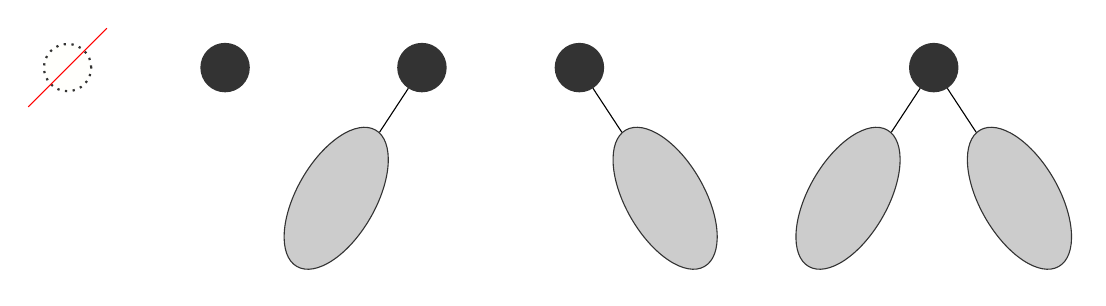
\begin{tikzpicture}[n/.style={draw=black!80, thick,fill=black!80, circle, minimum size=0.6cm},
      t/.style={draw=black!80, ellipse, minimum height=2cm,minimum width=1cm, fill=black!20}]
      \draw node[n,dotted, fill=yellow!1] (t1) at (0,0) {};
      \draw[draw=red] (0.5,0.5) -- (-0.5,-0.5);

      \draw node[n] (t2) at (2,0) {};

      \draw node[n] (t3) at (4.5,0) {} node[t, below left=of t3,xshift=0.8cm, rotate=-30] (t31) {};
      \draw[draw] (t3) -- (t31);

      \draw node[n] (t4) at (6.5,0) {} node[t, below right=of t4,xshift=-0.8cm, rotate=30] (t41) {};
      \draw[draw] (t4) -- (t41);

      \draw node[n] (t5) at (11,0) {} node[t, below left=of t5,xshift=0.8cm, rotate=-30] (t51) {} node[t, below right=of t5,xshift=-0.8cm, rotate=30] (t52) {};
      \draw[draw] (t5) -- (t51);
      \draw[draw] (t5) -- (t52);
    \end{tikzpicture}
  }
\end{frame}

\begin{frame}[fragile]
  \frametitle{请观察二叉树, 并回答下列问题}

  \scalebox{0.7} {
    \begin{forest}
      [A, name=A
      [B, name=B [D [H] [I]] [E [J] [K]]]
      [C, name=C [F [L] [M]] [G [N] [O]]]
      ];
     \draw[draw, dotted, thick] (B.north) ++(-2cm, 0.2cm)-- ++(9cm, 0cm)
     node[above, right, yshift=0.5cm]{1};
     \draw[draw, dotted, thick] (B.south) ++(-2cm, -0.2cm)-- ++(9cm, 0cm)
     node[above, right, yshift=0.5cm]{2};
     \draw[draw, dotted, thick] (B.south) ++(-2cm, -1.6cm)-- ++(9cm, 0cm)
     node[above, right, yshift=0.5cm]{3} node[below, right, yshift=-0.5cm] {4};
    \end{forest}
  }

  \begin{enumerate}
  \item 二叉树的第$i$层最多有多少个结点?
  \item 二叉树深度为k,则它最多有多少个结点?
  \item 二叉树有n个节点,请问它最小深度是几?
  \item 二叉树叶子的数目和度为2的节点的数目是否相等?如果不等,又是什么关系?
  \end{enumerate}
\end{frame}

\begin{frame}[fragile]
  \frametitle{二叉树的性质}
  \begin{itemize}
  \item 性质1: 二叉树的第$i$层至多有$2^{i-1}$个结点。
  \item 性质2: 深度为$k$的二叉树至多有$2^k-1$个结点($k \geq 1$)。
  \item \color{red} 性质3: 二叉树中终端结点数为$n_0$,度为2的结点数为$n_2$,则有$n_0 = n_2 + 1$
    (试证明)
  \end{itemize}
\end{frame}

\begin{frame}[fragile]
  \frametitle{二叉树的性质}
  二叉树中终端结点数为$n_0$,度为2的结点数为$n_2$,则有$n_0 = n_2 + 1$

  \begin{columns}[T,c]
    \begin{column}{0.6\linewidth}
      \begin{itemize}
      \item 设二叉树中度为1的结点数为$n_1$, 二叉树中总结点数为$N$,则有:
        
        $N = n_0 + n_1 + n_2$
      \item 再考虑二叉树中的分支数(每个节点有唯一一个入的分支,根节点除外;再考虑出
        的分支数量), 则有:

        $N - 1 =n_1 + 2 \times n_2$
      \item 整理可得:

        $n_0 = n_2 + 1$
      \end{itemize}
    \end{column}
    \begin{column}{0.35\linewidth}      
      \begin{forest}
        [{}, name=root,for tree={color=white,fill=black}
        [{}, name=n21, grow=-55 [{}, name=n31 [{~}] [{~}]]]
        [{}, name=n22, grow=235 [{}, name=n32,[{~}, draw=none,fill=none, no edge] [{~}]]]
        ]
      \end{forest}
    \end{column}
  \end{columns}
\end{frame}

\begin{frame}[fragile]
  \frametitle{完全二叉树}
  \begin{columns}[T]
    \column{0.55\textwidth}
    \begin{forest}
      [1, for tree={minimum width=1.8em, minimum height=1.8em}
      [2 [4 [8] [9]] [5 [10] [11]]]
      [3 [6 [12] [{}, no edge,draw=none]] [7]]
      ]
    \end{forest}
    \pause
    
    \column{0.4\textwidth}
    是否完全二叉树?

    \begin{forest}
      [1
      [2 [4] [5]]
      [3 [{}, no edge, draw=none] [7]]
      ]
    \end{forest}

    \pause
    
    \begin{forest}
      [1
      [2]
      [3 [6] [7]]
      ]
    \end{forest}
  \end{columns}
\end{frame}

\begin{frame}[fragile]
  \frametitle{试找出非完全二叉树}

  \begin{forest}
    [{}, for tree={fill=black}]
  \end{forest} \hspace{3cm}
  \begin{forest}
    [{}, for tree={fill=black} [{}] [{}]]
  \end{forest}
  
  \begin{forest}
    [{}, for tree={fill=black}
    [{} [{}] [{}]]
    [{}]]
  \end{forest}
  \begin{forest}
    [{}, for tree={fill=black}
    [{} [{} [{}] [{}]] [{}]]
    [{}]]
  \end{forest}
  \begin{forest}
    [{}, for tree={fill=black}
    [{} [{}] [{}]]
    [{} [{}] [{}]]]
  \end{forest}
  \begin{forest}
    [{}, for tree={fill=black}
    [{} [{} [{} [{}] [{}]] [{}]] [{}]]
    [{}]]
  \end{forest}
  \begin{forest}
    [{}, for tree={fill=black}
    [{} [{} [{}] [{}, no edge, draw=none, fill=none]] [{}]]
    [{} [{}] [{}]]]
  \end{forest}
\end{frame}



\begin{frame}[fragile]
  \frametitle{二叉树的性质}
  \begin{easylist}
  & 性质4:具有$n$个结点的完全二叉树的深度为:
    \[ \biggl\lfloor {log_2 n} \biggr\rfloor + 1 \] 
  \end{easylist}
  
  \small
  对于完全二叉树,设深度为$k$, 由$2^{k-1}-1 < n \leq 2^k - 1$可知,
  $2^{k-1} \leq n <2^k$, 则 $k-1 \leq log_2n < k$
  (参考性质2)
  
  \begin{columns}[T]
    \begin{column}{0.45\linewidth}      
      \scalebox{0.6}{
        \begin{forest}
          [1, for tree={minimum width=2.5em, minimum height=2.5em}
          [2 [4 [8] [9]] [5 [10] [11]]]
          [3 [6 [12] [13]] [7 [14] [15]]]
          ]
        \end{forest}
      }
      
      满二叉树
    \end{column}
    \begin{column}{0.45\linewidth}
      \scalebox{0.6}{
        \begin{forest}
          [1, for tree={minimum width=2.5em, minimum height=2.5em}
          [2 [4 [8] [9]] [5 [10] [11]]]
          [3 [6 [12] [{}, no edge, draw=none]] [7]]
          ]
        \end{forest}
      }
      
      完全二叉树
    \end{column}
  \end{columns}
\end{frame}







\begin{frame}[fragile]
  \frametitle{测试}

\begin{columns}[T]
  \column{0.6\textwidth}
    对于完全二叉树:
  \begin{enumerate}
  \item 若完全二叉树有叶子结点出现在第$k$层,它可能还有(~~~~~~)层的叶子结点;
  \item 若某结点的右子树的最大层次为$L$,则其左子树的最大层次为(~~~~~~~~);
  \item 若按如图所示的编号方式,试求出编号为$i$的节点的父节点和子节点的编号.
  \end{enumerate}

  \column{0.36\textwidth}
  \scalebox{0.6}{
    \begin{forest}
      [1
      [2 [4 [8] [9]] [5 [10] [11]]]
      [3 [6 [12] [{}, no edge,draw=none]] [7]]
      ]\
    \end{forest}
  }
\end{columns}

\pause
\begin{enumerate}
\item $k-1$, $k+1$
\item $L$ or $L+1$
\end{enumerate}
\end{frame}


\begin{frame}[fragile]
  \frametitle{二叉树的性质}
  \begin{center}
    \scalebox{0.6} {
      \begin{forest}
        [1, name=A,for tree={}
        [2, name=B [4 [8] [9]] [5 [10] [11]]]
        [3, name=C [6 [12] [{}, no edge,draw=none] ] [7] ]
        ]
        \draw[draw, dotted, thick] (B.north) ++(-2cm, 0.2cm)-- ++(9cm, 0cm)
        node[above, right, yshift=0.5cm]{1};
        \draw[draw, dotted, thick] (B.south) ++(-2cm, -0.2cm)-- ++(9cm, 0cm)
        node[above, right, yshift=0.5cm]{2};
        \draw[draw, dotted, thick] (B.south) ++(-2cm, -1.6cm)-- ++(9cm, 0cm)
        node[above, right, yshift=0.5cm]{3} node[below, right, yshift=-0.5cm] {4};
      \end{forest}
    }
  \end{center}

  \begin{itemize}
  \item 性质5: 对具有$n$个结点的完全二叉树的结点按层次顺序编号,对任意结点$i$有:
    \begin{itemize}
    \item (有关结点$i$的双亲)若$i=1$,则为二叉树的根结点, 没有双亲;否则双亲结点的
      编号为: $\biggl\lfloor{\dfrac{i}{2}}\biggr\rfloor$
    \item (有关结点$i$的孩子) 若$n<2 \cdot i$, 则结点$i$无左孩子;否则左孩子编号
      是$2 \cdot i$。
    \item 若$n<2 \cdot i+1$,则结点i无右孩子;否则右孩子编号为$2 \cdot i+1$
    \end{itemize}
  \end{itemize}
\end{frame}


\begin{frame}[t,fragile]
  \frametitle{二叉树的存储结构:顺序存储}
  \begin{columns}
    \begin{column}[T]{0.45\textwidth}
        \scalebox{0.6} {
          \begin{forest}
            [1, name=A,for tree={color=white,fill=black}
            [2, for tree={dotted,color=black,fill=white}, [4 [8] [9]] [5 [10] [11]]]
            [3, name=C [6 [12] [{}, no edge,draw=none, fill=none] ] [7] ]
            ]
          \end{forest}
        }

        \vspace{2cm}
        \scalebox{0.6}{
          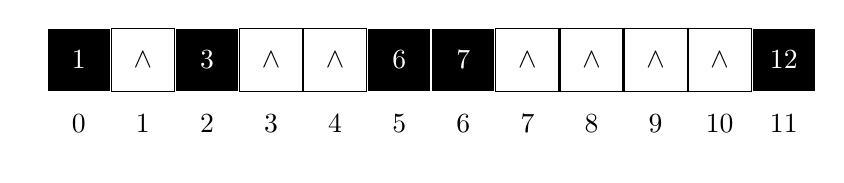
\begin{tikzpicture}[ n/.style={minimum size=0.8cm}]
            \draw node[] (n0) {};
            \foreach \x  [evaluate = \x as \xp using int(\x-1)] in {1, ..., 12}
            \draw node[n, right=0 of n\xp](n\x) {\xp};


            \foreach \x in {2,4,5,8,9,10,11}
            \draw node[n, above=0 of n\x, draw] (d\x) { $\wedge$};

            \foreach \x/\y in {1/1,3/3,6/6,7/7,12/12}
            \draw node[n, above=0 of n\x, draw,white, fill=black](d\x) {\y};
          \end{tikzpicture}
        }

    \end{column}

    \begin{column}[T]{0.55\textwidth}
      \begin{minted}[bgcolor=yellow!20, fontsize=\scriptsize]{c}
#define MAX_SIZE 100
typedef int SqBiTree[MAX_SIZE];
SqBiTree bt;
      \end{minted}

      \begin{minted}[bgcolor=red!5, fontsize=\scriptsize]{java}
class SqBiTree {
  //static int MAX_SIZE = 100;
  //int[] data = new int[MAX_SIZE];
  List<Integer> data = new ArrayList<>();
}
      \end{minted}
    \end{column}
  \end{columns}
  
  \begin{itemize}
  \item 把结点安排成一个恰当的序列(编号),存储在数组中
  \item 便于“随机存取”
  \end{itemize}
\end{frame}







\begin{frame}[fragile]
  \frametitle{二叉树的存储结构:顺序存储}
  \begin{itemize}
  \item 适用于完全二叉树
  \end{itemize}

  \begin{columns}
    \column{0.5\textwidth}
    \scalebox{0.8} {
      \begin{forest}
        [$a$, for tree={color=white,fill=black}
        [{}, draw=none, no edge, fill=none]
        [$b$
        [{}, draw=none, no edge, fill=none]
        [$c$ [{}, draw=none, no edge, fill=none] [$d$] ]
        ]
        ]
      \end{forest}
    }

    \column{0.4\textwidth}
    \scalebox{0.8} {
      \begin{forest}
        [1, for tree={color=white,fill=black}
        [2 [4] [5 [6] [7]]]
        [3]
        ]
      \end{forest}
    }
  \end{columns}

  \pause
  
  \scalebox{0.7}{
    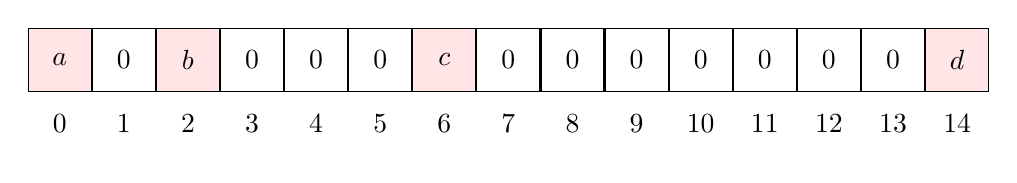
\begin{tikzpicture}[ n/.style={minimum size=0.8cm}]
      \draw node[n] (n0) {0};
      \foreach \x  [evaluate = \x as \xp using int(\x-1)] in {1, ..., 14}
      \draw node[n, right=0 of n\xp](n\x) {$\x$};

      \foreach \x in {1,3,4,5,7,8, ..., 13}
      \draw node[n, above=0 of n\x, draw](d\x) {$0$};

      \foreach \x/\y in {0/a,2/b,6/c,14/d}
      \draw node[n, above=0 of n\x, draw, fill=red!10](d\x) {$\y$};
    \end{tikzpicture}
  }

  \pause
  \hspace{4cm}
  \scalebox{0.7}{
    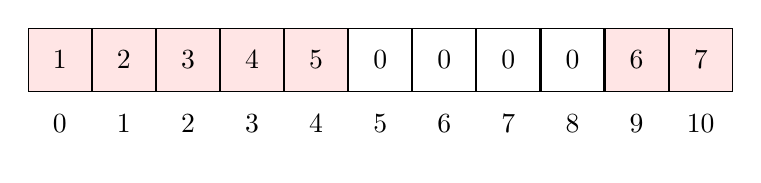
\begin{tikzpicture}[ n/.style={minimum size=0.8cm}]
      \draw node[n] (n0) {0};
      \foreach \x  [evaluate = \x as \xp using int(\x-1)] in {1, ..., 10}
      \draw node[n, right=0 of n\xp](n\x) {$\x$};

      \foreach \x in {5, ..., 8}
      \draw node[n, above=0 of n\x, draw](d\x) {$0$};

      \foreach \x/\y in {0/1,1/2,2/3,3/4,4/5,9/6,10/7}
      \draw node[n, above=0 of n\x, draw, fill=red!10](d\x) {$\y$};
    \end{tikzpicture}
  }
\end{frame}

\begin{frame}[fragile]
  \frametitle{二叉树的链式存储:二叉链表}
  \begin{columns}[T]
    \column{0.4\textwidth}
    \scalebox{0.7}{
      \begin{forest}
        [1
        [2 [{}, no edge, draw=none] [4 [5] [6]]]
        [3]]
      \end{forest}
    }
    \column{0.4\textwidth}
    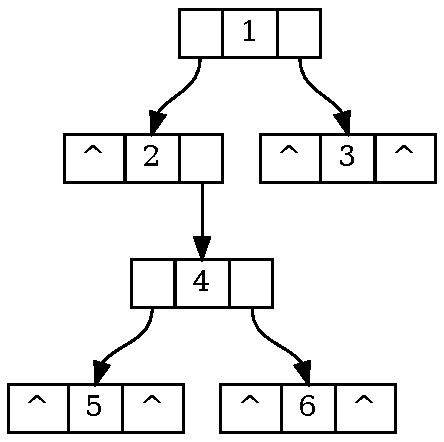
\includegraphics[width=0.6\textwidth]{dot/tree-store-bilink.pdf}
  \end{columns}

  \small
  \begin{columns}
    \column{0.48\textwidth}
    \begin{minted}[fontsize=\scriptsize,bgcolor=red!5]{c}
typedef struct BiTNode  { // C Code
  ElemType data;
  struct BiTNode *lchild, *rchild;
} BiTNode, *BiTree;
    \end{minted}

    \column{0.48\textwidth}
    \begin{minted}[fontsize=\scriptsize,bgcolor=yellow!10]{c}
class BiTNode<T> { //Java Code
  T data;
  BiTNode lchild, rchild;
}
    \end{minted}
  \end{columns}

  思考:含$n$个结点的二叉链表中有多少个空指针?

  \pause
  指针域一共有$2*n$个,分支共有$N-1$,  每个分支占用一个指针域,所以空指针数量为:  $2*n - (n-1) = n+1$
\end{frame}

\begin{frame}[fragile]
  \frametitle{二叉树的链式存储:三叉链表}
  \begin{itemize}
  \item 二叉链表不便查找父节点, 可加一个指向双亲的指针
  \end{itemize}

  \begin{columns}[T]
    \column{0.5\textwidth}
    \scalebox{0.5}{
      \begin{forest}
        [1
        [2 [{}, no edge, draw=none] [4 [5] [6]]]
        [3]]
      \end{forest}
    }
    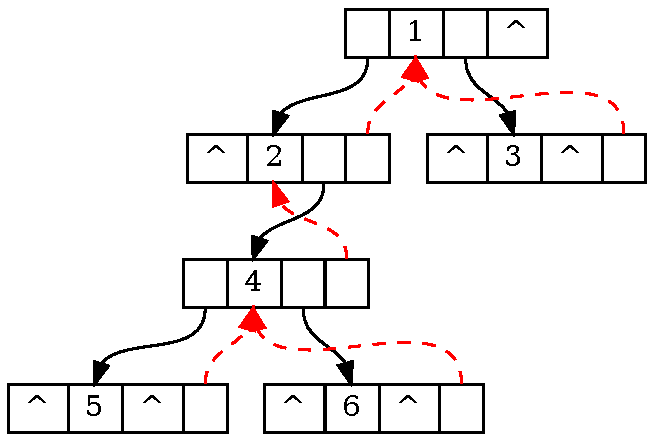
\includegraphics[width=0.8\textwidth]{dot/tree-store-trilink.pdf}
    
    \column{0.5\textwidth}
    \begin{minted}[fontsize=\scriptsize,bgcolor=red!5]{c}
typedef struct BiTNode  { // C Code
  ElemType data;
  struct BiTNode *lchild, *rchild;
  struct BiTNode *parent;
} BiTNode, *BiTree;
    \end{minted}

    \begin{minted}[fontsize=\scriptsize,bgcolor=yellow!10]{c}
class BiTNode<T> { //Java Code
  T data;
  BiTNode lchild, rchild, parent;
}
    \end{minted}
  \end{columns}

  \small 思考: 有n个结点的三叉链表有多少个空指针?

  \pause
  \scriptsize
  对于二叉链表,指针域一共有$2*n$个,分支共有$N-1$,  每个分支占用一个指针域,所以空指针数量为$2*n - (n - 1) = n+1 $;  对于parent,根节点无父节点,所以共有$n+1+1=n+2$个空指针
\end{frame}


\begin{frame}[fragile, plain]
  ~  
\end{frame}


\subsection{遍历二叉树和线索二叉树}
\begin{frame}[fragile]
  \frametitle{遍历二叉树和线索二叉树}

  在二叉树的一些应用中,常常要求在树中查找具有某种特征的结点,或者对树中全部结点逐
  一进行某种处理。这就引入了遍历二叉树的问题,即如何按某条搜索路径巡访树中的每一个
  结点,使得每一个结点均被访问一次且仅访问一次。
\end{frame}

\begin{frame}[fragile]
  \frametitle{二叉树的遍历}
 \begin{itemize}
 \item 遍历是指按某种方式访问所有结点,使每个结点被访问一次且只被访问一次。
 \item 二叉树的遍历是按一定规则将二叉树的结点排成一个线性序列,即非线性序列线性
   化。
 \item 遍历的方式: 深度优先和广度优先,深度优先又分为三种:
   \begin{itemize}
   \item 先序次序
   \item 中序次序(对称序次序)
   \item 后序次序 
   \end{itemize}
 \end{itemize} 
\end{frame}

\begin{frame}[fragile]
  \frametitle{二叉树的遍历}
  \begin{easylist}
    & 1、先序遍历二叉树的操作定义为: 若二叉树为空,则空操作;否则
    && (1)访问根结点;
    && (2)先序遍历左子树;
    && (3)先序遍历右子树。
    & 2、中序遍历二叉树的操作定义为:若二叉树为空,则空操作;否则
    && (1)中序遍历左子树;
    && (2)访问根结点;
    && (3)中序遍历右子树。
    & 3、后序遍历二叉树的操作定义为:若二叉树为空,则空操作;否则
    && (1)后序遍历左子树;
    && (2)后序遍历右子树;
    && (3)访问根结点。
  \end{easylist}
\end{frame}

\begin{frame}[fragile]
  \frametitle{示例}
  \scalebox{0.8}{
    \begin{forest}
      [A
      [B [D] [{}, no edge, draw=none]]
      [C [E [{}, no edge, draw=none] [G]] [F [H] [I]]]
      ]
    \end{forest}
  }

  \pause
  \begin{itemize}
  \item 先序:ABDCEGFHI
  \item 中序:DBAEGCHFI
  \item 后序:DBGEHIFCA
  \item 广度优先:ABCDEFGHI
  \end{itemize}
\end{frame}

\begin{frame}[fragile]
  \frametitle{二叉树的遍历}
  \begin{columns}[T]
    \column{0.6\textwidth}
    //先序遍历二叉树递归算法C伪代码
    \begin{minted}[bgcolor=red!5, fontsize=\small]{c}
status preOrderTraverse(BiTree T){
  if(T){
    printf(T->data);
    preOrderTraverse(T->lchild);
    preOrderTraverse(T->rchild);
  }
}
    \end{minted}
    \begin{itemize}
    \item status代表什么?
    \item printf代表什么?
    \end{itemize}

    \column{0.4\textwidth}
    \scalebox{0.8}{
      \begin{forest}
        [A
        [B [D] [{}, no edge, draw=none]]
        [C [E [{}, no edge, draw=none] [G]] [F [H] [I]]]
        ]
      \end{forest}
    }    
  \end{columns}
\end{frame}


\begin{frame}[fragile]
  \frametitle{二叉树的遍历}
  \begin{columns}[T]
    \column{0.6\textwidth}
    先序遍历递归算法的Java实现
  
    \begin{minted}[bgcolor=yellow!10,fontsize=\small]{java}
class Node {
  String data;
  Node left, right;
}
class Tree {
  void preOrderTraverse(Node node) {
    if(node != null) {
      System.out.println(node.data);
      preOrderTraverse(node.left);
      preOrderTraverse(node.right);
    }
  }
}
    \end{minted}

    \column{0.4\textwidth}
    \scalebox{0.8}{
      \begin{forest}
        [A
        [B [D] [{}, no edge, draw=none]]
        [C [E [{}, no edge, draw=none] [G]] [F [H] [I]]]
        ]
      \end{forest}
    }
  \end{columns}
\end{frame}

\begin{frame}[fragile, allowframebreaks]
  \frametitle{中序遍历的Java实现}
  \begin{minted}[fontsize=\scriptsize]{java}
public class Tree {
  Node root;

  public Tree(Node root) {
    this.root = root;
  }

  void inOrderTraverse() {
    inOrderTraverse(root);
  }

  void inOrderTraverse(Node node) {
    if(node != null) {
      inOrderTraverse(node.lc);
      //visit(node);
      System.out.println(node);
      inOrderTraverse(node.rc);
    }
  }

  public static void main(String[] args) {
    Node a  =new Node("A",
    new Node("B", new Node("D"), null),
    new Node("C", new Node("E"), new Node("F"))
    );
    Tree tree = new Tree(a);
    tree.inOrderTraverse();
  }

  static class Node {
    String data;
    Node lc, rc;

    public Node(String data, Node lc, Node rc) {
      this.data = data;
      this.lc = lc;
      this.rc = rc;
    }

    public Node(String data) {
      this.data = data;
      this.lc = null;
      this.rc = null;
    }

    public String toString(){
      return data;
    }
  }
}
  \end{minted}
\end{frame}

\begin{frame}[fragile]
  \frametitle{如下将得到树的什么序列?}
  \begin{columns}[T]
    \column{0.6\textwidth}
    \begin{minted}[bgcolor=yellow,fontsize=\small]{c}
status traverse(BiTree T) {
  InitStack(S);
  p = T;
  while(p || !StackEmpty(S)) {
    if(p) {
      push(S, p); p = p->lchild;
    } else {
      pop(S, p);
      printf(p->data);
      p = p->rchild;
    }
  }
  return OK;
}
    \end{minted}

    \column{0.4\textwidth}
    \scalebox{0.8}{
      \begin{forest}
        [A
        [B [D] [{}, no edge, draw=none]]
        [C [E [{}, no edge, draw=none] [G]] [F [H] [I]]]
        ]
      \end{forest}
    }
  \end{columns}  
\end{frame}


\begin{frame}[fragile]
  \frametitle{如下将得到树的什么序列?}
  \begin{columns}[T]
    \column{0.6\textwidth}
    \begin{minted}[bgcolor=yellow!10,fontsize=\small]{c}
void traverse(TreeNode root) {
  Stack stack = new Stack();
  TreeNode p = root;
  while(p!=null || stack.notEmpty()) {
    if(p!=null) {
      stack.push(p);
      p = p.lchild;
    } else {
      p = stack.pop();
      printf(p.data);
      p = p.rchild;
    }
  }
}
    \end{minted}

    \column{0.4\textwidth}
    \scalebox{0.8}{
      \begin{forest}
        [A
        [B [D] [{}, no edge, draw=none]]
        [C [E [{}, no edge, draw=none] [G]] [F [H] [I]]]
        ]
      \end{forest}
    }
  \end{columns}  
\end{frame}

\begin{frame}[fragile]
  \frametitle{二叉树的遍历:广度优先}
  \begin{columns}[T]
    \column{0.6\textwidth}
    算法步骤:
    \begin{itemize}
    \item 访问节点
    \item 从左到右依次访问儿子节点
    \item 重复前一步骤
    \end{itemize}
    
    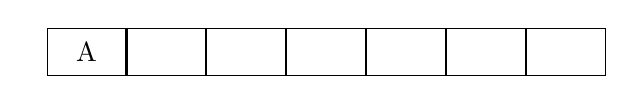
\begin{tikzpicture}[ n/.style={minimum width=1cm,minimum height=0.6cm, draw}]
      \draw node[] (n0) {};
      \foreach \x  [evaluate = \x as \xp using int(\x-1)] in {1, ..., 7}
      \draw node[n, right=0 of n\xp](n\x) {};
      
      \draw node[n, right=0 of n0] {A};
    \end{tikzpicture}

    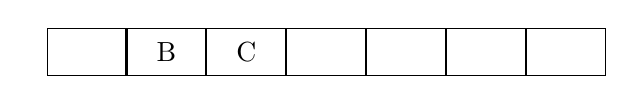
\begin{tikzpicture}[ n/.style={minimum width=1cm,minimum height=0.6cm, draw}]
      \draw node[] (n0) {};
      \foreach \x  [evaluate = \x as \xp using int(\x-1)] in {1, ..., 7}
      \draw node[n, right=0 of n\xp](n\x) {};
      
      \draw node[n, right=0 of n1] {B} node[n, right=0 of n2]{C};
    \end{tikzpicture}

    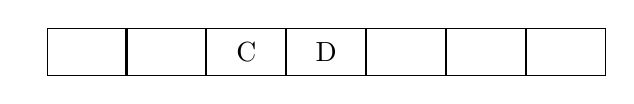
\begin{tikzpicture}[ n/.style={minimum width=1cm,minimum height=0.6cm, draw}]
      \draw node[] (n0) {};
      \foreach \x  [evaluate = \x as \xp using int(\x-1)] in {1, ..., 7}
      \draw node[n, right=0 of n\xp](n\x) {};
      
      \draw node[n, right=0 of n2] {C} node[n, right=0 of n3]{D};
    \end{tikzpicture}

    .......

    课堂练习:编程实现广度优先遍历。
    
    \column{0.4\textwidth}
    \scalebox{0.8}{
      \begin{forest}
        [A
        [B [D] [{}, no edge, draw=none]]
        [C [E [{}, no edge, draw=none] [G]] [F [H] [I]]]
        ]
      \end{forest}
    }
  \end{columns}
  
\end{frame}

\begin{frame}[fragile]
  \frametitle{广度优先遍历}
  \begin{minted}{java}
void bfs(TreeNode root) {
  Queue Q = new Queue();
  Q.enqueue(root);
  while(Q.notEmpty()) {
    TreeNode node = Q.dequeue();
    printf(node);
    if(node.left!=null) Q.enqueue(node.left);
    if(node.right !=null) Q.enqueue(node.right);
  }
}
  \end{minted}
\end{frame}


\begin{frame}[fragile]
  \frametitle{补充}
  \begin{itemize}
  \item 由一棵给定的二叉树可以获得三种遍历序列,同样,也可以由这些遍历序列来重新构
    造二叉树。
  \item 举例
    
    先序:ABCDEFGHIJ
    
    中序:CBDEAFHIGJ
  \item 由于不能从遍历序列中区分二叉树的左、右子树,因此单用一个遍历序列是无法构造
    二叉树的。利用中序遍历序列,并结合先序遍历序列或后序遍历序列就能重新构造二叉
    树。
  \end{itemize}
\end{frame}

\begin{frame}[fragile]
  \frametitle{二叉树的线索化}
  \begin{itemize}
  \item 基于二叉链表可以很方便地查找节点的左、右孩子。
  \item 问题:如何快速查找给定结点在遍历所得线性序列中的前驱和后继。
  \item 该信息在遍历的动态过程中才能得到。如果经常需要查找前驱和后继,需要在二叉链
    表的结点上添加指向前驱和后继的指针,叫做{\color{red}线索}。这样得到的二叉树称
    为{\color{red}线索二叉树}。
  \end{itemize}
\end{frame}

\begin{frame}[fragile]
  \frametitle{举例:中序线索二叉树}
  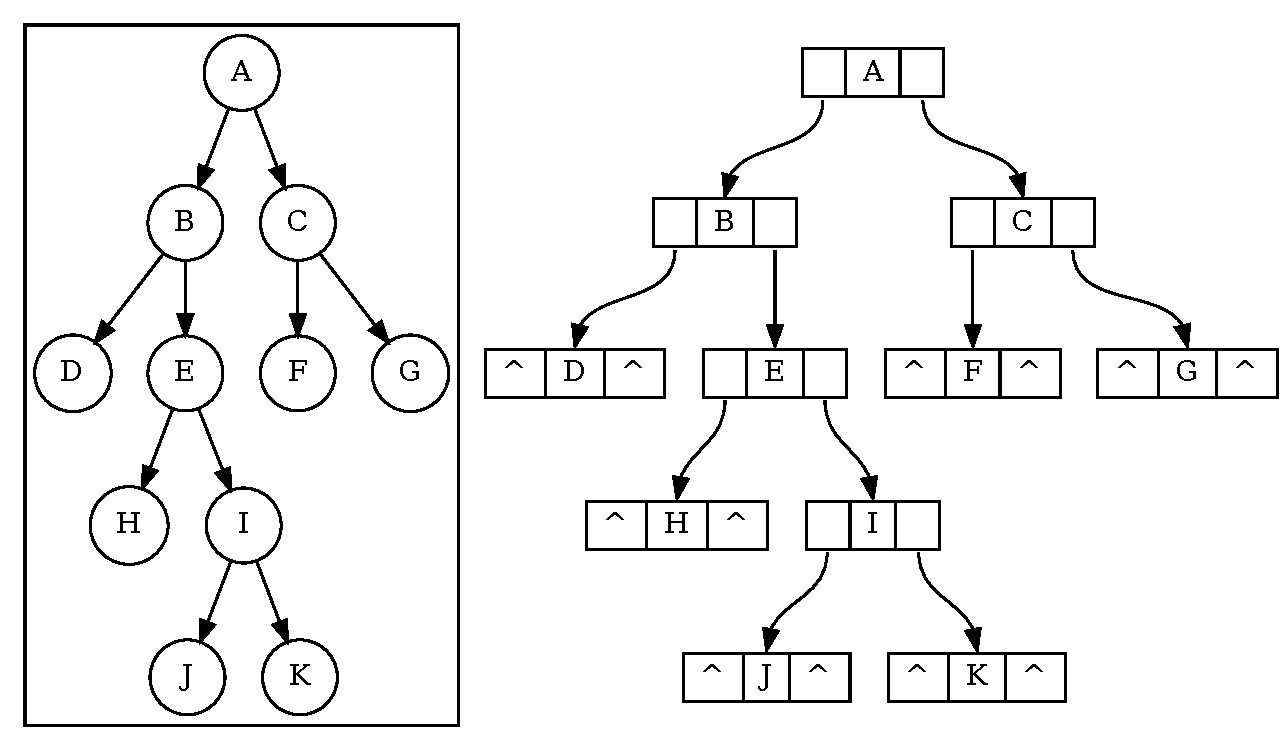
\includegraphics[width=0.6\textwidth]{dot/tree-thread.pdf}
  \begin{itemize}
  \item 以右图二叉树为例,中序序列为(~~~~~~~~~~~).
  \item 线索的表示:若结点有左子树,则指向其左孩子,否则指向其前驱;若节点有右子树,则指向
    其右孩子,否则指向其后继。
  \item 请问结点A和F的前驱和后继分别是?
  \end{itemize}
\end{frame}

\begin{frame}[fragile]
  \frametitle{举例:中序线索二叉树}
  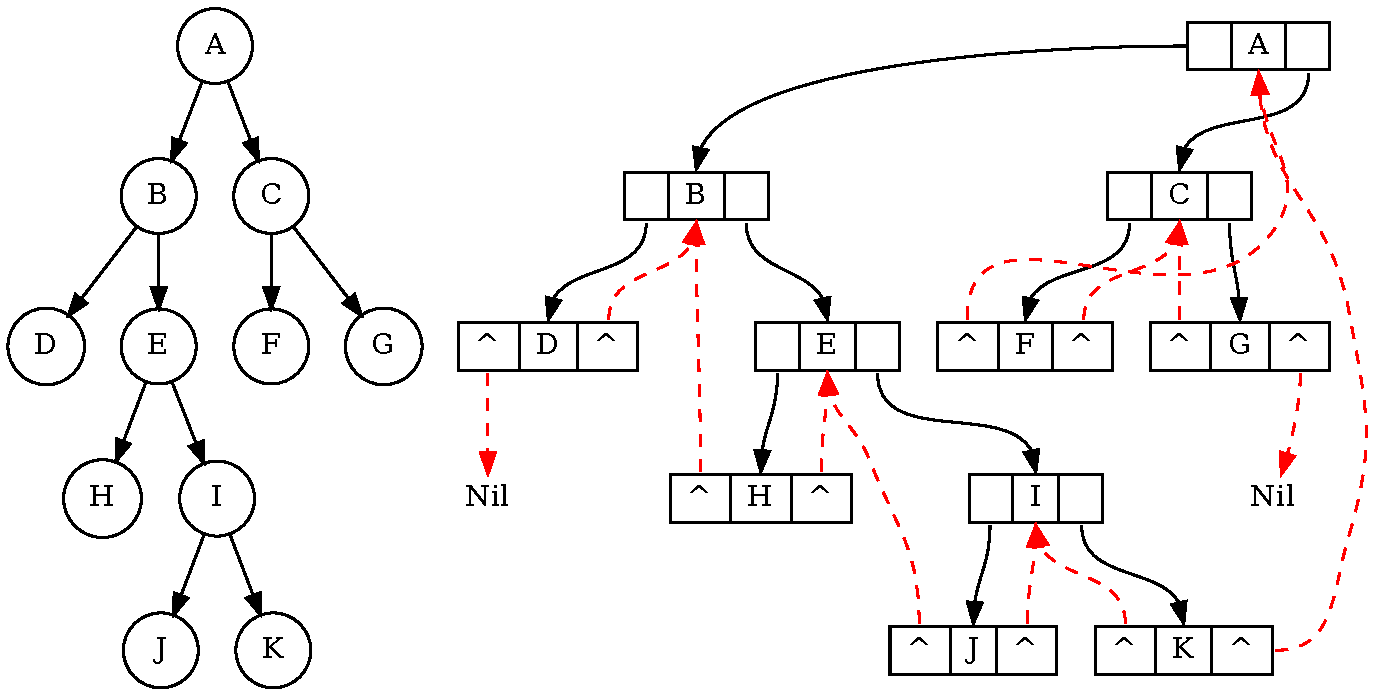
\includegraphics[width=0.9\textwidth]{dot/tree-thread2.pdf}
\end{frame}

\begin{frame}[fragile]
  \frametitle{带头节点的中序线索链表}
  参照双向链表,在二叉树线索链表上添加头节点,令头节点的左孩子指向二叉树的根节点。
  优点:既可从第一个结点起顺后继遍历,也可从最后一个结点起顺前驱遍历。
  
  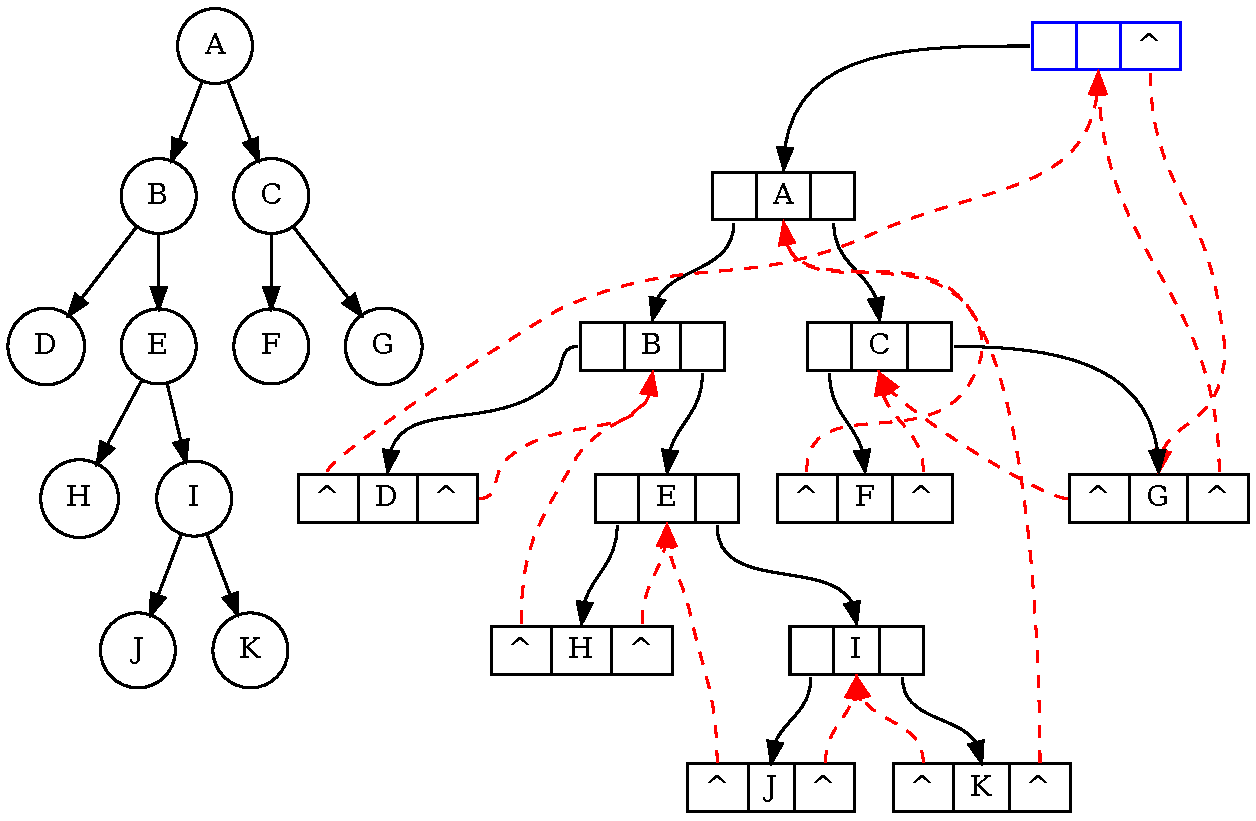
\includegraphics[width=0.7\textwidth]{dot/tree-thread3.pdf}
\end{frame}

\begin{frame}[fragile]
  \frametitle{练习}
  画出下图的先序、中序和后序线索二叉树。

  \begin{forest}
    [A
    [B [D [{}, no edge, draw=none] [G]] [{}, no edge, draw=none]]
    [C [E] [F]]
    ]
  \end{forest}
\end{frame}

\begin{frame}[fragile, plain]
  ~  
\end{frame}

\subsection{树和森林}
\begin{frame}[fragile]
  \frametitle{树和森林}
  \begin{itemize}
  \item 树的存储结构
  \item 树和二叉树的转换
  \item 森林和二叉树的转换
  \item 树和森林的遍历
  \end{itemize}
\end{frame}

\begin{frame}[fragile]
  \frametitle{树的存储结构:双亲表示法}
  \begin{columns}[T]
    \column{0.5\textwidth}
    \begin{forest}
      [R, for tree={edge={draw, <-}} [A [C] [D] [E]] [B [F]]]
    \end{forest}

    \vspace{1cm}
    \scalebox{0.6}{
      \begin{tikzpicture}[ n/.style={minimum size=0.8cm}]
        \draw node[n] (n0) {结点索引} node[n,above=0 of n0](label) {标记} node[n,above=0 of label,xshift=-0.5cm] {父结点索引};
        \foreach \x  [evaluate = \x as \xp using int(\x-1)] in {1, ..., 7}
        \draw node[n, right=0 of n\xp](n\x) {$\xp$};

        \foreach \x/\y in {1/R,2/A,3/B,4/C, 5/D, 6/E, 7/F}
        \draw node[n, above=0 of n\x, draw](n\x) {$\y$};

        \foreach \x/\y in {1/{-},2/0,3/0,4/1, 5/1, 6/1, 7/2}
        \draw node[n, above=0 of n\x, draw](n\x) {$\y$};
      \end{tikzpicture}
    }

    \column{0.5\textwidth}

    \begin{minted}[bgcolor=red!5, fontsize=\scriptsize]{java}
class PtNode<T> {
  T data;
  int parent;
}
    \end{minted}

    \begin{minted}[bgcolor=yellow!10, fontsize=\scriptsize]{c}
typedef struct{
  telemtype data;
  int parent;
} PtNode;
    \end{minted}
    
    因节点的度各异,从父亲指向孩子极不方便!若经常需要查找孩子结点,双亲表示法就不方
    便了。
  \end{columns}
\end{frame}

\begin{frame}[fragile]
  \frametitle{树的存储结构:孩子表示法}
  \begin{columns}[T]
    \column{0.5\textwidth}
    \scalebox{0.7}{
      \begin{forest}
        [R, for tree={edge={draw, <-}} [A [C] [D] [E]] [B [F]]]
      \end{forest}
    }

    \small 把每个结点的孩子结点排列成一个线性表,以单链表做存储结构.

    \scalebox{0.6}{
      \begin{tikzpicture}[ n/.style={minimum height=0.8cm, minimum width=1cm},
        n2/.style={minimum height=0.6cm, minimum width=0.7cm, fill=red!5},
        e/.style={->, very thick}]
        \draw node[n] (n0) {索引} node[n,right=0 of n0](label) {标记/父结点};
        \foreach \x  [evaluate = \x as \xp using int(\x-1)] in {1, ..., 7}
        \draw node[n, below=0 of n\xp](n\x) {$\xp$};

        \foreach \x/\y/\z in {1/R/,2/A/,3/B/,4/C/$\wedge$, 5/D/$\wedge$, 6/E/$\wedge$, 7/F/$\wedge$}
        \draw node[n, right=0 of n\x, draw, fill=yellow!10](\y) {$\y$} node[n, right=0 of \y, draw] (P\y) {\z};

        \draw node[n2, draw, right=of PR] (c11) {1} node[n2, draw, right=0 of c11] (c12) {};
        \draw node[n2, draw, right=of c12] (c21) {2} node[n2, draw, right=0 of c21] (c22) {$\wedge$};
        \draw[e] (PR.center) -- (c11) (c12.center)--(c21);        

        \draw node[n2, draw, right=of PA] (c11) {3} node[n2, draw, right=0 of c11] (c12) {};
        \draw node[n2, draw, right=of c12] (c21) {4} node[n2, draw, right=0 of c21] (c22) {};
        \draw node[n2, draw, right=of c22] (c31) {5} node[n2, draw, right=0 of c31] (c32) {$\wedge$};

        \draw[e] (PA.center) -- (c11) (c12.center)--(c21) (c22.center)--(c31);        

        \draw node[n2, draw, right=of PB] (c11) {6} node[n2, draw, right=0 of c11] (c12) {$\wedge$};
        \draw[e] (PB.center) -- (c11);
      \end{tikzpicture}
    }

    \column{0.5\textwidth}

    试写出ChildNode, CTree \pause
    
    \begin{minted}[breaklines, bgcolor=red!5, fontsize=\scriptsize]{java}
class TNode<T> {
  T data;
  ChildNode firstChild;
}

class ChildNode<T> {
  int index;
  ChildNode nextSibling;
}

class Tree {
  TNode<String>[] nodes = new TNode<String>[]{new TNode("R"), new TNode("A")};
  TNode root = nodes[0];
}
    \end{minted}
  \end{columns}
\end{frame}

\begin{frame}[fragile]
  \frametitle{树的存储结构:双亲+孩子表示法}

  \scalebox{0.7}{
    \begin{forest}
      [R, for tree={edge={draw, <-}} [A [C] [D] [E]] [B [F]]]
    \end{forest}
  }

  \scalebox{0.6}{
    \begin{tikzpicture}[ n/.style={minimum height=0.8cm, minimum width=1cm},
      n2/.style={minimum height=0.6cm, minimum width=1cm, fill=red!5},
      e/.style={->, very thick}]
      \draw node[n] (n0) {索引} node[n,right=0 of n0](label) {标记/父结点};
      \foreach \x  [evaluate = \x as \xp using int(\x-1)] in {1, ..., 7}
      \draw node[n, below=0 of n\xp](n\x) {$\xp$};

      \foreach \x/\y/\t/\z in {1/R/-1/,2/A/0/,3/B/0/,4/C/1/$\wedge$, 5/D/1/$\wedge$, 6/E/1/$\wedge$, 7/F/2/$\wedge$}
      \draw node[n, right=0 of n\x, draw, fill=yellow!10](\y) {$\y$} 
      node[n, right=0 of \y, draw, fill=red!20] (T\y) {\t}
      node[n, right=0 of T\y, draw] (P\y) {\z};

      \draw node[n2, draw, right=of PR] (c11) {1} node[n2, draw, right=0 of c11] (c12) {};
      \draw node[n2, draw, right=of c12] (c21) {2} node[n2, draw, right=0 of c21] (c22) {$\wedge$};
      \draw[e] (PR.center) -- (c11) (c12.center)--(c21);        

      \draw node[n2, draw, right=of PA] (c11) {3} node[n2, draw, right=0 of c11] (c12) {};
      \draw node[n2, draw, right=of c12] (c21) {4} node[n2, draw, right=0 of c21] (c22) {};
      \draw node[n2, draw, right=of c22] (c31) {5} node[n2, draw, right=0 of c31] (c32) {$\wedge$};

      \draw[e] (PA.center) -- (c11) (c12.center)--(c21) (c22.center)--(c31);        

      \draw node[n2, draw, right=of PB] (c11) {6} node[n2, draw, right=0 of c11] (c12) {$\wedge$};
      \draw[e] (PB.center) -- (c11);
    \end{tikzpicture}
  }
\end{frame}

\begin{frame}[fragile]
  \frametitle{树的存储结构:孩子兄弟表示法}

  试想如何借鉴二叉树的存储方法?

  树和森林的存储结构与算法都很复杂,如果能够将它们转换为二叉树,不但可以采用二叉树
  的存储结构,而且可以利用二叉树的有关算法来实现有关操作。幸运的是,树或森林与二叉
  树之间存在一一对应关系。
\end{frame}

\begin{frame}[fragile]
  \frametitle{树的存储结构:孩子兄弟表示法}
  使用二叉链表, 两个指针分别指向第一个孩子和下一个兄弟.
  
  \begin{minted}[bgcolor=red!5, fontsize=\scriptsize]{java}
class CSNode<T> {
  T data;
  CSNode<T> firstChild, nextSibling;
}  
  \end{minted}

  \begin{columns}[T]
    \column{0.2\textwidth}
    ~
    
    \column{0.3\textwidth}
    \scalebox{0.7}{
      \begin{forest}
        [R [A [C] [D] [E]] [B [F]]]
      \end{forest}
    }

    \column{0.2\textwidth}
    \vspace{1cm} {\Huge{$\Rightarrow$}}

    \column{0.3\textwidth}
    \scalebox{0.7}{
      \begin{forest}
        [R
        [A
        [C [{}, no edge, draw=none] [D [{},no edge, draw=none] [E]]]
        [B [F] [{}, no edge, draw=none]]]
        [{}, no edge, draw=none]]
      \end{forest}
    }
  \end{columns}
\end{frame}

\begin{frame}[fragile]
  \frametitle{树与二叉树的转换}
  \begin{itemize}
  \item 孩子作左子树的根,兄弟作右子树的根
  \item 任何一棵树对应的二叉树,其右子树必空,也就是说,所有的树都可以转化为二叉
    树,但不是所有的二叉树都可以转化为树。
  \end{itemize}

  \begin{columns}[T]
    \column{0.2\textwidth}
    ~
    \column{0.3\textwidth}
    \scalebox{0.7}{
      \begin{forest}
        [A [B] [C] [D]]
      \end{forest}
    }

    \column{0.2\textwidth}
    \vspace{1cm} {\Huge{$\Leftrightarrow$}}

    \column{0.3\textwidth}
    \scalebox{0.7}{
      \begin{forest}
        [A
        [B [{}, no edge, draw=none] [C [{},no edge, draw=none] [D]]]
        [{}, no edge, draw=none]]
      \end{forest}
    }
  \end{columns}
\end{frame}

\begin{frame}[fragile]
  \frametitle{森林与二叉树的转换}
  \begin{itemize}
  \item 零棵或有限棵不相交的树的集合称为森林。自然界中树和森林是不同的概念,但在数
    据结构中,树和森林只有很小的差别——任何一棵树,删去根结点就变成了森林。
  \item 根据树的二叉链表表示,任何一棵和树对应的二叉树的右子树必空。若将森林中第二
    棵树的根结点看成第一棵树的根结点的兄弟,则可以导出森林和二叉树的对应关系。
  \end{itemize}
\end{frame}

\begin{frame}[fragile]
  \frametitle{森林与二叉树的转换示例}
  \begin{columns}[T]
    \column{0.6\textwidth}
  \scalebox{0.8}{
  \begin{tabular}{c c c}
    \begin{forest}
      [A [C] [D] [E]]
    \end{forest} &
    \begin{forest}
      [B [F]]
    \end{forest} &
    \begin{forest}
      [G [H] [I [J]]]
    \end{forest} \\
    \huge{$\downarrow$} & \huge{$\downarrow$} & \huge{$\downarrow$}  \\
    \begin{forest} 
      [A [C [{}, no edge, draw=none] [D [{}, no edge, draw=none] [E]]] [{}, no edge, draw=none]]
    \end{forest} &
    \begin{forest}
      [B [F] [{}, no edge, draw=none]]
    \end{forest} &
    \begin{forest}
      [G [H [{}, no edge, draw=none] [I [J] [{}, no edge, draw=none]]] [{}, no edge, draw=none]]
    \end{forest}
  \end{tabular}
  }

  \column{0.4\textwidth}
  \pause
  \scalebox{0.7}{
    \begin{forest}
      [A
      [C [{}, no edge, draw=none] [D [{}, no edge, draw=none] [E]]]
      [B [F]  [G [H [{}, no edge, draw=none] [I [J] [{}, no edge, draw=none]]] [{}, no edge, draw=none]]]]
    \end{forest}
  }
  \end{columns}
\end{frame}

\begin{frame}[fragile]
  \frametitle{树和森林的遍历}
  \small
  请按下述原则写出该树的遍历序列
  \begin{itemize}
  \item 先根遍历: =相应二叉树的先序遍历
    
    首先访问根结点;再从左到右遍历根结点的每一棵子树。

  \item 后根遍历: =相应二叉树的中序遍历

    首先 按照从左到右的顺序后根遍历根结点的每一棵子树,再访问根结点。
    
  \end{itemize}

  请画出该树对应的二叉树,并写出该二叉树的先、中、后序遍历

  \begin{columns}[T]
    \column{0.4\textwidth}
    \hspace{1cm}
    \scalebox{0.8} {
      \begin{forest}
        [A [B [E] [F]] [C] [D [G]]]
      \end{forest}
    }
    \column{0.6\textwidth}
    \pause
    上图的先根遍历序列为:A B E F C D G \\
    上图的后根遍历序列为:E F B C G D A
  \end{columns}
\end{frame}

\begin{frame}[fragile]
  \frametitle{森林的遍历}
  \small
  \begin{easylist}
    & 前序遍历(相应二叉树的先序遍历)
    && 访问森林中第一棵树的根结点;
    && 先根遍历第一棵树的根结点的子树;
    && 先根遍历去掉第一棵树后的子森林。
    & 中序遍历(相应二叉树的中序遍历)
    && 后根遍历第一棵树的根结点的子树;
    && 访问森林中第一棵树的根结点;
    && 后根遍历去掉第一棵树后的子森林。
  \end{easylist}

  \begin{columns}
    \column{0.5\textwidth}
    \scalebox{0.6}{
      \begin{tabular}{c c c}
        \begin{forest}
          [A [B]]
        \end{forest} &
                       \begin{forest}
                         [C [D] [E] [F]]
                       \end{forest} &
                                      \begin{forest}
                                        [G [H [J]] [I [K]]]
                                      \end{forest}
      \end{tabular}
    }

    \column{0.5\textwidth}
    前序遍历结果: A B C D E F G H J I K
    
    中序遍历结果:B A D E F C J H K I G
  \end{columns}
\end{frame}

\begin{frame}[fragile, plain]
  ~  
\end{frame}

\subsection{哈夫曼树}
\begin{frame}[fragile]
  \frametitle{哈夫曼树}
  \small
  \begin{itemize}
  \item Huffman coding (哈夫曼编码) 是David A. Huffman于1952年在麻省理工攻读博士
    时发明的一种编码方法,可用于无损数据压缩的熵编码。 Huffman编码广泛应用在涉及数
    字压缩和传输的领域,如fax、modem、计算机网络和HDTV。
  \item 原理:使用一张特殊的编码表将源字符进行编码,它的特殊之处在于它是根据每一个
    源字符出现的估算概率建立起来的——出现概率高的字符使用较短的编码,反之出现概率低
    的则使用较长的编码,使编码后的字符串的平均期望长度降低,从而达到无损压缩数据的
    目的。若能比较准确的估计英文中各个字母出现概率,就能大幅提高无损压缩的效率。
  \item 例如,在英文中,用普通的表示方法时,每个英文字母均占用一个字节(byte),即8位。
    实际上,e的出现概率很高,而z的出现概率则最低。当利用哈夫曼编码进行压缩时,e可能
    用1位来表示,z可能用25位。
  \end{itemize}
\end{frame}

\begin{frame}[fragile]
  \frametitle{David Huffman (1925/08/09 -- 1999/10/07)}
  \begin{itemize}
  \item 1950年,Huffman在MIT的信息理论与编码研究生班学习。Robert Fano教授让学生们
    自己决定是参加期未考试还是做一个大作业,因为大作业比期末考试可能更容易通
    过,Huffman选择了后者。正是一个大作业促使了Huffman算法的诞生!
  \item 离开MIT后,Huffman来到University of California, Santa Cruz的计算机系任
    教,并为此系的学术做出了许多杰出的工作。而他的算法也广泛应用于传真机,图象压缩
    和计算机安全领域。但是Huffman却从未为此算法申请专利或其它能够为他带来经济利益
    的东西,他将他全部的精力放在教学上,用他自己的话来说,“My products are my
    students.”
  \item David Huffman对于有限状态自动机,开关电路,异步过程和信号设计也做出了杰出贡
    献。
  \end{itemize}
\end{frame}

\begin{frame}[fragile]
  \frametitle{举例:假设学生成绩分布如下,试构造一棵树}
  \begin{tabular}{|c|c|c|c|c|c|}
    \hline
    Grade & Bad & Pass & General & Good & Excellent \\ \hline
    Score & 0 -- 59 & 60 -- 69 & 70 -- 79 & 80 -- 89 & 90 -- 100 \\ \hline
    Ratio & 0.05 & 0.15 & 0.40 & 0.30 & 0.10 \\ \hline
  \end{tabular}

  \scalebox{0.6}{
    \begin{forest}
      [$s<60$, for tree={draw=none}
      [Bad,,edge label={node[midway,right,font=\scriptsize]{Y}}]
      [$s<70$,edge label={node[midway,right,font=\scriptsize]{N}} [Pass] [$s<80$ [General] [$s<90$ [Good] [Excellent]]]]
      ]
    \end{forest}
  }
  \scalebox{0.7}{
    \begin{forest}
      [$s<80$, for tree={draw=none}
      [$s<70$,edge label={node[midway,right,font=\scriptsize]{Y}} [$s<60$ [Bad]
      [Pass]] [General]]
      [$s<90$,edge label={node[midway,right,font=\scriptsize]{N}} [Good] [Excellent] ]]
    \end{forest}
  }
  Which one is better?
\end{frame}

\begin{frame}[fragile, plain]

  \begin{tabular}{|c|c|c|c|c|c|}
    \hline
    Grade & Bad & Pass & General & Good & Excellent \\ \hline
    Score & 0 -- 59 & 60 -- 69 & 70 -- 79 & 80 -- 89 & 90 -- 100 \\ \hline
    Ratio & 0.05 & 0.15 & 0.40 & 0.30 & 0.10 \\ \hline
  \end{tabular}

  \begin{columns}[T]
    \column{0.25\textwidth}
    \scalebox{0.6}{
      \begin{forest}
        [$s<60$, for tree={draw=none}
        [Bad,,edge label={node[midway,right,font=\scriptsize]{Y}}]
        [$s<70$,edge label={node[midway,right,font=\scriptsize]{N}} [Pass] [$s<80$ [General] [$s<90$ [Good] [Excellent]]]]
        ]
      \end{forest}
    }

    \column{0.75\textwidth}
    \begin{itemize}
    \item 结点的带权路径长度(Weighted Path Length):

      \[WPL(good) = 4*0.3=1.2 \]
      
    \item 树的带权路径长度:
      \begin{equation*}
        \begin{array}{r c l}
          WPL(TREE) & = & 1 \times 0.05  \\
          & & + 2 \times 0.15 \\
          & & + 3 \times 0.40 \\
          & & + 4 \times 0.30 \\
          & & + 4 \times 0.10 \\
          & = & 3.15 \\
        \end{array}
      \end{equation*}
    \end{itemize}
  \end{columns}
\end{frame}

\begin{frame}[fragile]
  \frametitle{练习:求树的带权路径长度}

  \begin{center}
    \begin{tabular}{|c|c|c|c|c|c|}
      \hline
      Grade & Bad & Pass & General & Good & Excellent \\ \hline
      Score & 0 -- 59 & 60 -- 69 & 70 -- 79 & 80 -- 89 & 90 -- 100 \\ \hline
      Ratio & 0.05 & 0.15 & 0.40 & 0.30 & 0.10 \\ \hline
    \end{tabular}
    
    \scalebox{0.6}{
      \begin{forest}
        [$s<60$, for tree={draw=none}
        [Bad,,edge label={node[midway,right,font=\scriptsize]{Y}}]
        [$s<70$,edge label={node[midway,right,font=\scriptsize]{N}} [Pass] [$s<80$ [General] [$s<90$ [Good] [Excellent]]]]
        ]
      \end{forest}
    }
  \end{center}
\end{frame}

\begin{frame}[fragile]
  \frametitle{哈夫曼树}具有最小带权路径长度的二叉树称为哈夫曼树(最优二叉树)。

  \begin{columns}[T]
    \column{0.55\textwidth}
    \scalebox{0.6}{
      \begin{forest}    
        for tree={ minimum width=0.6cm }    
        [{~} [{~} [2] [3]] [{~} [4] [7]]]       
      \end{forest}
    }

    $WPL=2\times 2 + 2\times 3 + 2 \times 4 + 2 \times 7 = 32$

    \scalebox{0.6}{
      \begin{forest}
        for tree={ minimum width=0.6cm } 
        [{~} [2] [{~} [3] [{~} [4] [7]]]]       
      \end{forest}
    }

    $WPL=1 \times 2 + 2\times 3 + 3 \times 4 + 3 \times 7 = 41$
    
    \column{0.55\textwidth}
    \pause
    \scalebox{0.6}{
      \begin{forest}
        for tree={ minimum width=0.6cm } 
        [{~} [7] [{~} [4] [{~} [3] [2]]]]
      \end{forest}
    }
    
    $WPL= 30$
  \end{columns}
\end{frame}


\begin{frame}[fragile]
  \frametitle{哈夫曼树的构造}

  由给定的$n$个权值$\{w_1, w_2, \cdots, w_n\}$,构造$n$棵只有一个叶子结点的二叉
  树 , 从而得到一个二叉树的集合$F=\{T_1, T_2, \cdots, T_n\}$.

  \begin{enumerate}
  \item 在$F$中选取根结点的权值最小和次小的两棵二叉树作为左、右子树构造一棵新的二叉
    树,这棵新的二叉树根结点的权值为其左、右子树根结点权值之和;
  \item 在集合$F$中删除作为左、右子树的两棵二叉树,并将新建立的二叉树加入到集合
    $F$中;
  \item 重复(2)、(3)两步,当$F$中只剩下一棵二叉树时,这棵二叉树便是所要建立的哈夫曼
    树。
  \end{enumerate}
\end{frame}

\begin{frame}[fragile]
  \frametitle{例子}
  1, 3, 5, 7
\end{frame}

\begin{frame}[fragile]
  \frametitle{课堂作业}
  \begin{columns}
    \column{0.3\textwidth}
    \scalebox{0.6}{
      \begin{forest}
        [A
        [B [D] [{}, no edge, draw=none]]
        [C [E [{}, no edge, draw=none] [G]] [F [H] [I]]]
        ]
      \end{forest}
    }

    \begin{minted}{java}
class TNode {
  String data;
  int lc, rc;
}
    \end{minted}

    \column{0.3\textwidth}
    \begin{tabular}{| c | c | c | c|}
      \hline
      0 & A & 1 & 2 \\ \hline
      1 & B & 3 & -1 \\ \hline
      2 & C & 4 & 5 \\ \hline
      3 & D & -1 & -1 \\ \hline
      4 & E & -1 & 6 \\ \hline
      5 & F & 7 & 8 \\ \hline
      6 & G & -1 & -1 \\ \hline
      7 & H & -1 & -1 \\ \hline
      8 & I & -1 & -1 \\ \hline
    \end{tabular}

    \column[T]{0.35\textwidth}
    \begin{itemize}
    \item 给定树$T$如图所示, 请写递归程序实现如下功能:
    \item (1)遍历树T,显示其先序/中序/后序 序列;
    \item (2)求结点数、叶子数;
    \item (3)求树T的深度.
    \end{itemize}
  \end{columns}
\end{frame}

\begin{frame}[fragile]
  \frametitle{本章作业}
  哈夫曼编码

  \begin{easylist}
    &   根据26个英文字母的频度,为每一个字母赋予一个唯一的最优编码

    & 输出要求, 每行一个字母,及其对应编码,如:

    && A: 00100
    && B: 0001
    && ...
  \end{easylist}
\end{frame}


\begin{frame}[fragile]
  \frametitle{英文字母的频率表}

  \begin{tabular}{|c | c || c | c || c | c| }
    \hline
    字母  & 出现频率 &  字母  & 出现频率  & 字母  & 出现频率 \\ \hline
    a & 8.167\% & j & 0.153\% & s & 6.327\% \\ \hline
    b & 1.492\% & k & 0.772\% & t & 9.056\% \\ \hline
    c & 2.782\% & l & 4.025\% & u & 2.758\% \\ \hline
    d & 4.253\% & m & 2.406\% & v & 0.978\% \\ \hline
    e & 12.702\% &  n & 6.749\% & w & 2.360\% \\ \hline
    f & 2.228\% & o & 7.507\% & x & 0.150\% \\ \hline
    g & 2.015\% & p & 1.929\% & y & 1.974\% \\ \hline
    h & 6.094\% & q & 0.095\% & z & 0.074\% \\ \hline
    i & 6.966\% & r & 5.987\% &    ~ &    \\ \hline
  \end{tabular}
\end{frame}

% \section{Graph}

\begin{frame}[fragile]{Graph}
  \begin{adjustbox}{max totalsize={.9\textwidth}{.7\textheight},center}
    \tikzstyle{every node}=[circle, draw, fill=black!50,
    inner sep=0pt, minimum width=4pt]
    % Tutte's 8-cage
    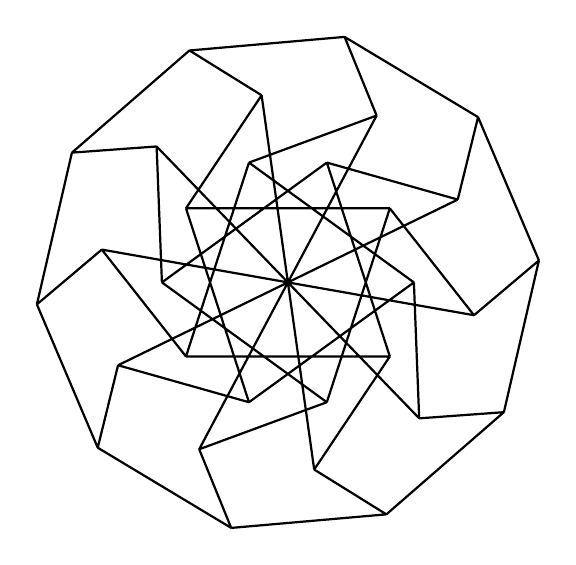
\begin{tikzpicture}[thick,scale=0.8]
      \draw \foreach \x in {0,36,...,324}
      {
        (\x:2) node {}  -- (\x+108:2)
        (\x-10:3) node {} -- (\x+5:4)
        (\x-10:3) -- (\x+36:2)
        (\x-10:3) --(\x+170:3)
        (\x+5:4) node {} -- (\x+41:4)
      };
    \end{tikzpicture}\quad

    % The largest 3-regular graph of diameter 3
    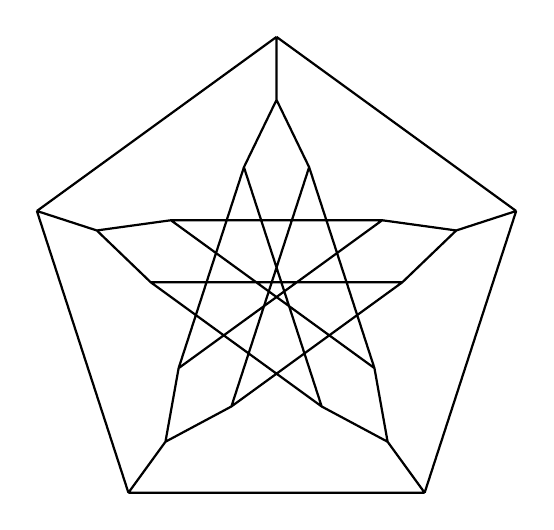
\begin{tikzpicture}[thick,scale=0.8]%
      \draw \foreach \x in {18,90,...,306} {
        (\x:4) node{} -- (\x+72:4)
        (\x:4) -- (\x:3) node{}
        (\x:3) -- (\x+15:2) node{}
        (\x:3) -- (\x-15:2) node{}
        (\x+15:2) -- (\x+144-15:2)
        (\x-15:2) -- (\x+144+15:2)
      };
    \end{tikzpicture}
  \end{adjustbox}
\end{frame}

\begin{frame}[fragile]{Content}
  \begin{easylist} \easyitem
    & 图的定义
    & 图的存储表示
    & 图的遍历
    & 图的连通性
  \end{easylist}
\end{frame}

\begin{frame}[fragile]
  \frametitle{图的用途}
  \begin{easylist}
    & 用数学语言来说,网络通常被视为一种加权图(Weighted Graph),其中节点(Node)代表实体,边(Edge)代表实体间的关系,而边的权重(Weight)则代表了这种关系的某种度量(如距离、成本、流量等)。

    & 除了数学上的定义,网络还具有实际的物理含义,它是从相同类型的实际问题中抽象出来的模型。这些实际问题包括但不限于交通系统、物流运输、通信系统等,因此习惯上会根据其应用领域称之为相应的网络类型,如交通网络、运输网络、通信网络等。

    & 现实生活中的许多问题,如交通路线的优化、ERP(企业资源规划)系统的工作计划制定等,都可以借助图与网络的模型进行建模和求解。这些模型能够帮助我们更好地理解和分析问题的本质,从而找到有效的解决方案。
  \end{easylist}
\end{frame}

\begin{frame}[fragile]
  \frametitle{社会网络(social network)}
  \small
  \begin{easylist}
    & 社会网络是指由社会个体成员之间因互动而形成的相对稳定的关系体系。
    & 社会网络分析(SNA)作为社会学的一个重要分支,自上世纪30年代末起逐步发展,成为研究社会结构的重要方法和技术。从30年代到60年代,这一领域吸引了来自心理学、社会学、人类学以及数学、物理、统计、概率等领域的学者,他们共同推动了SNA的理论、方法和技术的发展,使其成为研究社会结构的重要范式。
  \end{easylist}
\end{frame}

\begin{frame}[fragile, allowframebreaks]
  \frametitle{六度分隔(Six Degrees of Separation)}
  \small
  \begin{easylist}
    & 六度空间理论(也称为小世界现象或六度分隔理论)最初是在1929年由匈牙利作家弗里奇斯·卡林思(Frigyes Karinthy)在他的短篇小说中提出的,他提出世界上所有人都可以通过至多五个中间人联系起来。

    & 1967年,哈佛大学的社会心理学教授Stanley Milgram (1933-1984)进行了一项著名的实验来验证这一理论。他设计了一个连锁信件实验,从Nebraska和Kansas随机选择了300多名志愿者,请他们寄一封信函给指定的一名住在波士顿的股票经纪人。实验结果表明,有六十多封信函最终到达了目标人手中,并且这些信函在传递过程中经过的中间人的数目平均只有大约5个。这一发现验证了六度空间理论,并使其受到了全世界的广泛关注。

    \newpage
    
    & 此外,Milgram还发现了漏斗效应,即大部分的信件传递都是由少数几个“明星人物”完成的,这些人在社交网络中具有很高的连接性,能够更快地传递信息。

    & 六度空间理论不仅激发了学术界的深入研究,还催生了电影《六度空间》(又称《六度分离》或《连锁反应》)等文化产品,进一步增强了公众对这一理论的兴趣和认知。
  \end{easylist}
\end{frame}

\begin{frame}[fragile, allowframebreaks]
  \frametitle{150法则(Rule of 150)}
  \begin{easylist}
    & 从欧洲发源的“赫特兄弟会”是一个自给自足的农民自发组织,他们有一个不成文的
    严格规定:每当聚居人数超过150人的规模,他们就把它变成两个,再各自发展。

    & 150也被称为“邓巴数字(Dunbar’s number)”,该理论认为人的大脑新皮层大小有限,
    提供的认知能力只能使一个人维持与大约150人的稳定人际关系。

    & 把人群控制在150人以下似乎是管理人群的一个最佳和最有效的方式。早期中国移动的动
    感地带sim卡最多保存150个手机号,早期一个MSN帐号只能对应150个联系人。

    & 不管你认识多少人,或者与更多人建立了弱链接,那些强链接仍然在此次此刻符合
    150法则。这也符合“二八”法则,即80\%的社会活动可能被150个强链接所占有。
  \end{easylist}
\end{frame}

\begin{frame}[fragile, allowframebreaks]
  \frametitle{网络模型}
  \begin{easylist}
    & 随机网络:
    && 在交通网络中,随机网络可以模拟道路拥堵的情况。假设道路的连接(箭线)和交叉口(节点)的实现具有一定的随机性,这取决于交通流量、道路状况等多种因素。
    && 用途:随机网络用于描述那些节点和连接具有不确定性的系统。在交通网络中,随机网络模型可以帮助预测和规划交通流量,优化交通设计,减少拥堵。此外,随机网络还广泛应用于计算机科学、社会学、生物学等领域,用于模拟和分析各种复杂系统的行为。
    \newpage
    & 小世界网络
    && 社交网络可以看作是一个小世界网络。在社交网络中,虽然大多数人只与少数人保持紧密联系(短路径),但几乎每个人都可以通过少数几个熟人联系到网络中的任何其他人(小世界现象)。
    && 用途:小世界网络模型用于描述那些具有较短的平均路径长度和较高的聚类系数的网络。这种网络结构使得信息在网络中传播得非常快,因此小世界网络模型在信息传播、社交网络分析、推荐系统等领域具有广泛应用。此外,小世界网络还用于研究生物网络、神经网络等复杂系统的行为。
    \newpage
    & 无标度网络
    && 互联网可以看作是一个无标度网络。在互联网中,少数大型网站(Hub点)拥有大量的链接,而大多数网站只有少量的链接。这种网络结构使得互联网呈现出无标度性,即节点的连接数(度数)分布严重不均匀。
    && 用途:无标度网络模型用于描述那些具有严重不均匀分布特性的网络。在互联网中,无标度网络模型有助于理解网络的拓扑结构、稳定性和鲁棒性等特性。此外,无标度网络还广泛应用于社交网络、金融网络、生物网络等领域的研究,以揭示这些复杂系统的内在规律和运行机制。
  \end{easylist}
\end{frame}

\begin{frame}[fragile]
  \frametitle{图(Graph)}
  \begin{itemize}
  \item 图$G=(V, E)$, $V$是顶点(Vertex)集合,$E$是边/弧(Edge/Arc)的集合.
  \item 顶点的度、出度和入度
  \end{itemize}

  \begin{columns}[T]
    \column{0.5\textwidth}
    有向图:
    
    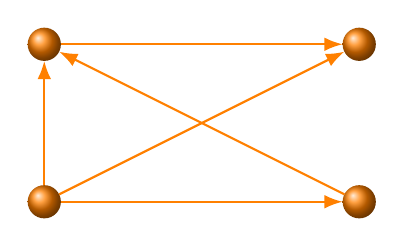
\begin{tikzpicture}[scale=1.0]
      \GraphInit[vstyle=Art]
      \Vertex{A}
      \Vertex[x=4,y=0]{B}
      \Vertex[x=0,y=2]{C}
      \Vertex[x=4,y=2]{D}
      \Edge[style={-Latex}](A)(D)

      \Edges[style={-Latex}](A,B,C, D)
      \Edges[style={-Latex}](A, C)
    \end{tikzpicture}
    
    \column{0.5\textwidth}
    无向图:
    
    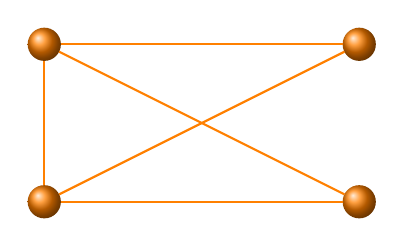
\begin{tikzpicture}[scale=1.0]
      \GraphInit[vstyle=Art]
      \Vertex{A}
      \Vertex[x=4,y=0]{B}
      \Vertex[x=0,y=2]{C}
      \Vertex[x=4,y=2]{D}
      \Edge[style={}](A)(D)

      \Edges[style={}](A,B,C, D)
      \Edges[style={}](A, C)
    \end{tikzpicture}
  \end{columns}
\end{frame}

\begin{frame}[fragile]
  \frametitle{图的相关概念}
  \includegraphics[width=0.9\textwidth]{figs/graph_concept.png}
\end{frame}

\begin{frame}[plain]
~  
\end{frame}

\begin{frame}[fragile]
  \frametitle{图的存储}
  如何表达下图的信息?
  \begin{columns}
    \column{0.4\textwidth}
    有向图:
    
    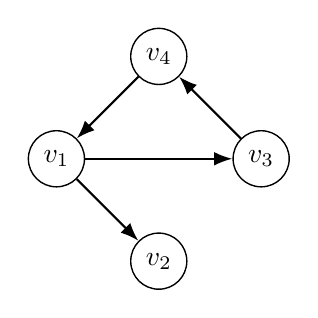
\begin{tikzpicture}[scale=1.3]
      \GraphInit[vstyle=Normal]
      \begin{scope}[rotate=180]
        \Vertices{circle}{$v_1$, $v_2$, $v_3$, $v_4$}
      \end{scope}
      \Edges[style={-Latex}]($v_1$,  $v_3$, $v_4$, $v_1$, $v_2$)
    \end{tikzpicture}
    
    \column{0.4\textwidth}
    无向图:
    
    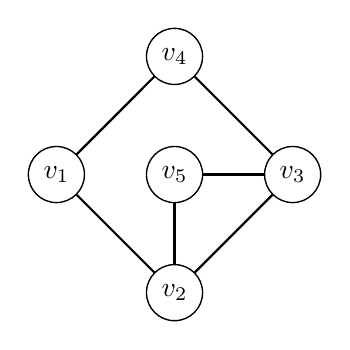
\begin{tikzpicture}[scale=1.5]
      \GraphInit[vstyle=Normal]
      \begin{scope}[rotate=180]
        \Vertices{circle}{$v_1$, $v_2$, $v_3$, $v_4$}
      \end{scope}
      \Vertex{$v_5$}
      \Edges($v_1$, $v_2$, $v_3$, $v_4$, $v_1$)
      \Edges($v_2$, $v_5$, $v_3$)
    \end{tikzpicture}
  \end{columns}
  
  \pause
  \begin{itemize}
  \item 可用邻接矩阵表达顶点及其关系。
  \end{itemize}
\end{frame}


\begin{frame}[fragile]
  \frametitle{图的存储}
  \small
  \begin{columns}[T]
    \column{0.4\textwidth}
    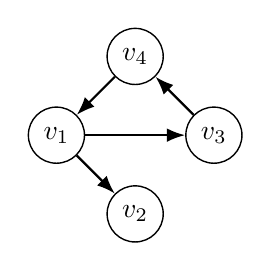
\begin{tikzpicture}[scale=1]
      \GraphInit[vstyle=Normal]
      \begin{scope}[rotate=180]
        \Vertices{circle}{$v_1$, $v_2$, $v_3$, $v_4$}
      \end{scope}
      \Edges[style={-Latex}]($v_1$,  $v_3$, $v_4$, $v_1$, $v_2$)
    \end{tikzpicture}
    \[
      \begin{blockarray}{ccccc}
         & v_1 & v_2 & v_3 & v_4 \\
        \begin{block}{c (c c c c)}
          v_1 & 0 & 1 & 1 & 0 \\
          v_2 & 0 & 0 & 0 & 0 \\
          v_3 & 0 & 0 & 0 & 1 \\
          v_4 & 1 & 0 & 0 & 0 \\
        \end{block}
      \end{blockarray}
    \]

    \column{0.4\textwidth}
    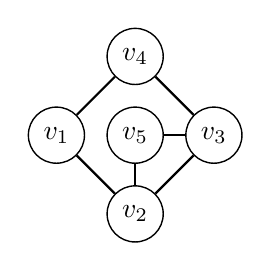
\begin{tikzpicture}[scale=1.0]
      \GraphInit[vstyle=Normal]
      \begin{scope}[rotate=180]
        \Vertices{circle}{$v_1$, $v_2$, $v_3$, $v_4$}
      \end{scope}
      \Vertex{$v_5$}
      \Edges($v_1$, $v_2$, $v_3$, $v_4$, $v_1$)
      \Edges($v_2$, $v_5$, $v_3$)
    \end{tikzpicture}

    \[
      \begin{blockarray}{cccccc}
         & v_1 & v_2 & v_3 & v_4 & v_5 \\
        \begin{block}{c (c c c c c)}
          v_1 & 0 & 1 & 0 & 1 & 0 \\
          v_2 & 1 & 0 & 1 & 0 & 1 \\
          v_3 & 0 & 1 & 0 & 1 & 1 \\
          v_4 & 1 & 0 & 1 & 0 & 0 \\
          v_5 & 0 & 1 & 1 & 0 & 0 \\
        \end{block}
      \end{blockarray}
    \]    
  \end{columns}
  
  \begin{itemize}
  \item 根据邻接矩阵,如何判断各顶点的度?
  \end{itemize}
\end{frame}

\begin{frame}[fragile]
  \frametitle{有向图的连续存储方式:邻接矩阵}
  \begin{columns}[T]
    \column{0.4\textwidth}
    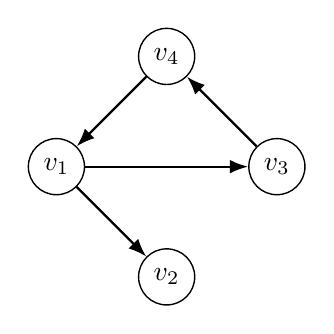
\begin{tikzpicture}[scale=1.4]
      \GraphInit[vstyle=Normal]
      \begin{scope}[rotate=180]
        \Vertices{circle}{$v_1$, $v_2$, $v_3$, $v_4$}
      \end{scope}
      \Edges[style={-Latex}]($v_1$,  $v_3$, $v_4$, $v_1$, $v_2$)
    \end{tikzpicture}
    \[
      \begin{blockarray}{ccccc}
        & v_1 & v_2 & v_3 & v_4 \\
        \begin{block}{c (c c c c)}
          v_1 & 0 & 1 & 1 & 0 \\
          v_2 & 0 & 0 & 0 & 0 \\
          v_3 & 0 & 0 & 0 & 1 \\
          v_4 & 1 & 0 & 0 & 0 \\
        \end{block}
      \end{blockarray}
    \]
    
    \column{0.6\textwidth}
    \begin{itemize}
    \item 建立二维数组$A[n][n]$, $n=|V|$
    \item 另需存放$n$个顶点信息
    \end{itemize}
  \end{columns}
\end{frame}

\begin{frame}[fragile]
  \frametitle{网的邻接矩阵}
  \begin{columns}[T]
    \column{0.4\textwidth}
    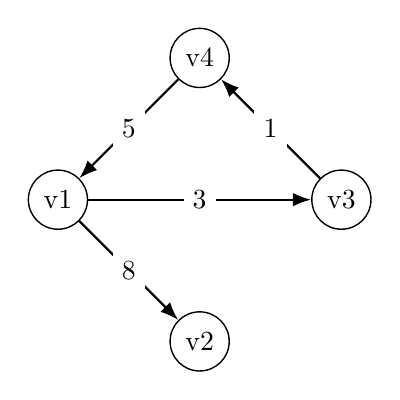
\begin{tikzpicture}[scale=1.8]
      \GraphInit[vstyle=Normal]
      \begin{scope}[rotate=180]
        \Vertices{circle}{v1, v2, v3, v4}
      \end{scope}
      \Edge[label = 8, style={-Latex}](v1)(v2)
      \Edge[label = 3, style={-Latex}](v1)(v3)
      \Edge[label = 5, style={-Latex}](v4)(v1)
      \Edge[label = 1, style={-Latex}](v3)(v4)
    \end{tikzpicture}
    \[
      \begin{blockarray}{ccccc}
        & v_1 & v_2 & v_3 & v_4 \\
        \begin{block}{c (c c c c)}
          v_1 & \infty & 8 & 3 & \infty \\
          v_2 & \infty & \infty & \infty & \infty \\
          v_3 & \infty & \infty & \infty & 1 \\
          v_4 & 5 & \infty & \infty & \infty \\
        \end{block}
      \end{blockarray}
    \]
    
    \column{0.6\textwidth}
    \begin{itemize}
    \item 有些图的边带有权重(常用来表示成本、距离、时间等), 这样的图称为:{\color{red} 网}。
    \item 网的邻接矩阵表达权重,没有边的顶点之间的权重默认为$\infty$
    \item 邻接矩阵表示方法非常直观、简单,但是会有什么问题? \pause
    \item 现实中的图经常对应稀疏矩阵,在这样情形下会有很大空间浪费.
    \end{itemize}
  \end{columns}  
\end{frame}

\begin{frame}[fragile]
  \frametitle{邻接表 (Adjacency List) -- 无向图}
  \begin{columns}[T]
    \column{0.35\textwidth}
    \begin{tikzpicture}[scale=1.3]
      \GraphInit[vstyle=Normal]
      \begin{scope}[rotate=90]
        \Vertices{circle}{v1, v2, v3, v4}
      \end{scope}
      \Edges(v3, v1, v2, v4)
    \end{tikzpicture}
    
    \column{0.6\textwidth}
    \scalebox{0.8}{
      \begin{tikzpicture}[ n/.style={minimum height=0.8cm, minimum width=1cm},
        n2/.style={minimum height=0.6cm, minimum width=1cm, fill=red!5},
        e/.style={->, very thick}]
        \draw node[n] (n0) {索引} node[n,right=0 of n0](label) {头节点};

        \foreach \x  [evaluate = \x as \xp using int(\x-1)] in {1, ..., 4}
        \draw node[n, below=0 of n\xp](n\x) {$\xp$};

        \foreach \x/\y/\z in {1/A/,2/B/,3/C/,4/D/}
        \draw node[n, right=0 of n\x, draw, fill=yellow!10](\y) {$v_\x$} node[n, right=0 of \y, draw] (P\y) {\z};


        \draw node[n2, draw, right=of PA] (c11) {2} node[n2, draw, right=0 of c11] (c12) {};
        \draw node[n2, draw, right=of c12] (c21) {1} node[n2, draw, right=0 of c21] (c22) {$\wedge$};
        \draw[e] (PA.center) -- (c11);
        \draw[e] (c12.center)--(c21);

        \draw node[n2, draw, right=of PB] (c11) {3} node[n2, draw, right=0 of c11] (c12) {};
        \draw node[n2, draw, right=of c12] (c21) {0} node[n2, draw, right=0 of c21] (c22) {$\wedge$};
        \draw[e] (PB.center) -- (c11) (c12.center)--(c21);

        \draw node[n2, draw, right=of PC] (c11) {0} node[n2, draw, right=0 of c11] (c12) {$\wedge$};
        \draw[e] (PC.center) -- (c11);

        \draw node[n2, draw, right=of PD] (c11) {1} node[n2, draw, right=0 of c11] (c12) {$\wedge$};
        \draw[e] (PD.center) -- (c11);
      \end{tikzpicture}
    }
  \end{columns}

  \begin{itemize}
  \item 无向图的邻接表:同一个顶点发出的边链接在同一个边链表中,便于确定顶点的度
  \item 需要$n$个头结点, $2e$个表结点
  \end{itemize}
\end{frame}

\begin{frame}[fragile]
  \frametitle{邻接表--有向图}
  \begin{columns}[T]
    \column{0.4\textwidth}
    \begin{tikzpicture}[scale=1.5]
      \GraphInit[vstyle=Normal]
      \begin{scope}[rotate=135]
        \Vertices{circle}{A, B, C, E}
      \end{scope}
      \Vertex{D}
      \Edges[style={-Latex}](A, B, C, D, E, A)
      \Edge[style={-Latex}](A)(D)	
    \end{tikzpicture}
    
    邻接表,便于确定节点出度

    \scalebox{0.7}{
      \begin{tikzpicture}[ n/.style={minimum height=0.8cm, minimum width=1cm},
        n2/.style={minimum height=0.6cm, minimum width=1cm, fill=red!5},
        e/.style={->, very thick}]
        \draw node[n] (n0) {索引} node[n,right=0 of n0](label) {头节点};

        \foreach \x  [evaluate = \x as \xp using int(\x-1)] in {1, ..., 5}
        \draw node[n, below=0 of n\xp](n\x) {$\xp$};

        \foreach \x/\y/\z in {1/A/,2/B/,3/C/,4/D/, 5/E/}
        \draw node[n, right=0 of n\x, draw, fill=yellow!10](\y) {$\y$} node[n, right=0 of \y, draw] (P\y) {\z};


        \draw node[n2, draw, right=of PA] (c11) {3} node[n2, draw, right=0 of c11] (c12) {};
        \draw node[n2, draw, right=of c12] (c21) {1} node[n2, draw, right=0 of c21] (c22) {$\wedge$};
        \draw[e] (PA.center) -- (c11);
        \draw[e] (c12.center)--(c21);

        \draw node[n2, draw, right=of PB] (c11) {2} node[n2, draw, right=0 of c11] (c12) {$\wedge$};
        \draw[e] (PB.center) -- (c11);

        \draw node[n2, draw, right=of PC] (c11) {3} node[n2, draw, right=0 of c11] (c12) {$\wedge$};
        \draw[e] (PC.center) -- (c11);

        \draw node[n2, draw, right=of PD] (c11) {4} node[n2, draw, right=0 of c11] (c12) {$\wedge$};
        \draw[e] (PD.center) -- (c11);

        \draw node[n2, draw, right=of PE] (c11) {0} node[n2, draw, right=0 of c11] (c12) {$\wedge$};
        \draw[e] (PE.center) -- (c11);
      \end{tikzpicture}
    }
    \pause
    
    \column{0.6\textwidth}
    逆邻接表,便于确定节点入度
    
    \scalebox{0.7}{
      \begin{tikzpicture}[ n/.style={minimum height=0.8cm, minimum width=1cm},
        n2/.style={minimum height=0.6cm, minimum width=1cm, fill=red!5},
        e/.style={->, very thick}]
        \draw node[n] (n0) {索引} node[n,right=0 of n0](label) {头节点};

        \foreach \x  [evaluate = \x as \xp using int(\x-1)] in {1, ..., 5}
        \draw node[n, below=0 of n\xp](n\x) {$\xp$};

        \foreach \x/\y/\z in {1/A/,2/B/,3/C/,4/D/, 5/E/}
        \draw node[n, right=0 of n\x, draw, fill=yellow!10](\y) {$\y$} node[n, right=0 of \y, draw] (P\y) {\z};

        \draw node[n2, draw, right=of PA] (c11) {4} node[n2, draw, right=0 of c11] (c12) {$\wedge$};
        \draw[e] (PA.center) -- (c11);

        \draw node[n2, draw, right=of PB] (c11) {0} node[n2, draw, right=0 of c11] (c12) {$\wedge$};
        \draw[e] (PB.center) -- (c11);

        \draw node[n2, draw, right=of PC] (c11) {1} node[n2, draw, right=0 of c11] (c12) {$\wedge$};
        \draw[e] (PC.center) -- (c11);

        \draw node[n2, draw, right=of PD] (c11) {2} node[n2, draw, right=0 of c11] (c12) {};
        \draw node[n2, draw, right=of c12] (c21) {0} node[n2, draw, right=0 of c21] (c22) {$\wedge$};
        \draw[e] (PD.center) -- (c11);
        \draw[e] (c12.center)--(c21);

        \draw node[n2, draw, right=of PE] (c11) {3} node[n2, draw, right=0 of c11] (c12) {$\wedge$};
        \draw[e] (PE.center) -- (c11);
      \end{tikzpicture}
    }    
  \end{columns}
\end{frame}

\begin{frame}[fragile]
  \frametitle{邻接表--权重处理}
  \scalebox{0.7}{
    \begin{tikzpicture}[scale=2]
      \GraphInit[vstyle=Normal]
      \begin{scope}[rotate=225]
        \Vertices{circle}{A, B, D, C}
      \end{scope}

      \Edge[style={-Latex}, label=1](A)(B)
      \Edge[style={-Latex, pos=0.2}, label=4](A)(D)

      \Edge[style={-Latex, pos=0.2, bend right}, label=9](B)(C)
      \Edge[style={-Latex}, label=2](B)(D)

      \Edge[style={-Latex}, label=3](C)(A)
      \Edge[style={-Latex, pos=0.2, bend right=10}, label=5](C)(B)
      \Edge[style={-Latex}, label=8](C)(D)

      \Edge[style={-Latex, bend right=40}, label=6](D)(C)
    \end{tikzpicture}
  }

  \scalebox{0.7}{
    \begin{tikzpicture}[ n/.style={minimum height=0.8cm, minimum width=1cm},
      n2/.style={minimum height=0.6cm, minimum width=1cm, fill=red!5},
      e/.style={->, very thick}]
      \draw node[n] (n0) {索引} node[n,right=0 of n0](label) {头节点};

      \foreach \x  [evaluate = \x as \xp using int(\x-1)] in {1, ..., 4}
      \draw node[n, below=0 of n\xp](n\x) {$\xp$};

      \foreach \x/\y/\z in {1/A/,2/B/,3/C/,4/D/}
      \draw node[n, right=0 of n\x, draw, fill=yellow!10](\y) {$\y$} node[n, right=0 of \y, draw] (P\y) {\z};

      \draw node[n2, draw, right=of PA] (c11) {1} node[n2, draw, right=0 of c11,fill=blue!10] (c12) {1} node[n2, draw, right=0 of c12] (c13) {};
      \draw node[n2, draw, right=of c13] (c21) {3}  node[n2, draw, right=0 of c21,fill=blue!10] (c22) {4} node[n2, draw, right=0 of c22] (c23) {$\wedge$};
      \draw[e] (PA.center) -- (c11);
      \draw[e] (c13.center) -- (c21);

      \draw node[above=of c11](tip1) {边的终点} node[right=of tip1](tip2){权重};
      \path[draw, ->] (tip1) edge (c11) (tip2) edge[bend right] (c12);
      
      \draw node[n2, draw, right=of PB] (c11) {3} node[n2, draw, right=0 of c11,fill=blue!10] (c12) {2} node[n2, draw, right=0 of c12] (c13) {};
      \draw node[n2, draw, right=of c13] (c21) {2}  node[n2, draw, right=0 of c21,fill=blue!10] (c22) {9} node[n2, draw, right=0 of c22] (c23) {$\wedge$};
      \draw[e] (PB.center) -- (c11);
      \draw[e] (c13.center) -- (c21);

      \draw node[n2, draw, right=of PC] (c11) {0} node[n2, draw, right=0 of c11,fill=blue!10] (c12) {3} node[n2, draw, right=0 of c12] (c13) {};
      \draw node[n2, draw, right=of c13] (c21) {1}  node[n2, draw, right=0 of c21,fill=blue!10] (c22) {5} node[n2, draw, right=0 of c22] (c23) {};
      \draw node[n2, draw, right=of c23] (c31) {3}  node[n2, draw, right=0 of c31,fill=blue!10] (c32) {8} node[n2, draw, right=0 of c32] (c33) {$\wedge$};
      \draw[e] (PC.center) -- (c11);
      \draw[e] (c13.center) -- (c21);
      \draw[e] (c23.center) -- (c31);

      \draw node[n2, draw, right=of PD] (c11) {2} node[n2, draw, right=0 of c11,fill=blue!10] (c12) {6} node[n2, draw, right=0 of c12] (c13) {$\wedge$};
      \draw[e] (PD.center) -- (c11);
    \end{tikzpicture}
  }
\end{frame}

\begin{frame}[fragile]
  \frametitle{练习}
  \begin{enumerate}
  \item 请写出数组存储和邻接表的类型定义
  \item 请在如下方面对比数组表示法和邻接表示法
    \begin{itemize}
    \item 存储表示是否唯一
    \item 空间复杂度
    \item 操作a: 求顶点$v_i$的度
    \item 操作b: 判定$(v_i, v_j)$是否是图的一条边
    \item 操作c: 通过遍历求边的数目
    \end{itemize}
  \end{enumerate}
\end{frame}
% TODO

\begin{frame}[fragile, allowframebreaks]
  \frametitle{邻接表表示}
  \scriptsize
  \begin{minted}{java}
    class VertexNode {
      String data;
      EdgeNode firstAdj = null;

      public VertexNode(String data) {
        this.data = data;
      }
    }

    class EdgeNode {
      int adjVertexNode;
      EdgeNode nextAdj = null;

      public EdgeNode(int vertexIdx) {
        this.adjVertexNode = vertexIdx;
      }

      public EdgeNode(int vertexIdx, EdgeNode nextAdj) {
        this.adjVertexNode = vertexIdx;
        this.nextAdj = nextAdj;
      }
    }
    
    public class Graph {
      VertexNode[] vertices;

      public void init() {
        this.vertices = new VertexNode[]{
          new VertexNode("v1"),
          new VertexNode("v2"),
          new VertexNode("v3"),
          new VertexNode("v4"),
          new VertexNode("v5"),
          new VertexNode("v6"),
          new VertexNode("v7"),
          new VertexNode("v8")
        };
        vertices[0].firstAdj = new EdgeNode(1, new EdgeNode(2));
        vertices[1].firstAdj = new EdgeNode(0, new EdgeNode(3, new EdgeNode(4)));
        vertices[2].firstAdj = new EdgeNode(0, new EdgeNode(5, new EdgeNode(6)));
        vertices[3].firstAdj = new EdgeNode(1, new EdgeNode(7));
        vertices[4].firstAdj = new EdgeNode(1, new EdgeNode(7));
        vertices[5].firstAdj = new EdgeNode(2, new EdgeNode(6));
        vertices[6].firstAdj = new EdgeNode(2, new EdgeNode(5));
        vertices[7].firstAdj = new EdgeNode(3, new EdgeNode(4));
      }
    }
  \end{minted}
\end{frame}

\begin{frame}[fragile]
  \frametitle{比较}
  \small
  \begin{tabular}{| p{2cm} | p{4cm} | p{4cm} |}
    \hline
    ~ & 数组表示法 & 邻接表法 \\ \hline
    表示结果 & 唯一 & 不唯一 \\ \hline
    空间复杂度 & $O(n^2)$ (适用于稠密图) & $O(n+e)$ (适用于稀疏图) \\ \hline
    无向图求顶点$v_i$的度 & 第$i$行(或第$i$列)上非零元素的个数 & 第$i$个边表中的结点个数 \\ \hline
    有向图求顶点$v_i$的度  & 第$i$行上非零元素的个数是$v_i$出度,第$i$列上非零元素的个数是$v_i$的入度 & 第$i$个边表上的结点个数,求入度还需遍历各顶点的边表。逆邻接表则相反\\ \hline
    判定$(v_i, v_j)$是否是图的一条边 &  看矩阵中的$i$行$j$列是否为0 & 扫描第i个边表 \\ \hline
    求边的数目 & 检测整个矩阵中的非零元所耗费的时间是$O(N^2)$ & 对每个边表的结点个数计数所耗费的时间是$O(e+n)$ \\ \hline
  \end{tabular}  
\end{frame}

\begin{frame}[fragile]
  \frametitle{思考}

  怎么把邻接表和逆邻接表相结合,同时表示出来?
\end{frame}

\begin{frame}[fragile]
  \frametitle{有向图的十字链表(Orthogonal List)}
  \begin{columns}[T]
    \column{0.4\textwidth}
    \scalebox{0.6}{
      \begin{tikzpicture}[
          % 定义样式
          node distance = 2cm,
          auto,
          every node/.style={
            circle,
            draw,
            font=\sffamily\Large\bfseries
          },
          edge/.style={draw,->,thick}
        ]
        % 定义节点
        \node (v0) at (0,0) {$v_0$};
        \node[right=of v0] (v1) {$v_1$};
        \node[below left=of v0] (v2) {$v_2$};
        \node[below right=of v0] (v3) {$v_3$};

        % 绘制边
        \path[edge] (v0) -- (v1);
        \path[edge, bend right] (v0) to (v2);
        \path[edge, bend right] (v2) to (v0);
        \path[edge] (v2) -- (v3);
        \path[edge] (v3) -- (v0);
        \path[edge] (v3) -- (v1);
      \end{tikzpicture}
    }
    \column{0.6\textwidth}
    将邻接表、逆邻接表结合起来.
    \begin{itemize}
    \item hlink: 指向弧头相同的下一条弧
    \item tlink: 指向弧尾相同的下一条弧
    \end{itemize}
  \end{columns}
  \scalebox{0.7}{
    \begin{tikzpicture}[ n/.style={minimum height=0.8cm, minimum width=1cm},
        n2/.style={minimum height=0.6cm, minimum width=1cm, fill=red!5},
        n3/.style={minimum height=0.6cm, minimum width=1cm},
        e/.style={->, thick, red},
        e2/.style={->, thick, blue}]
      \draw node[n] (n0) {索引} node[n,right=0 of n0](label) {头节点};

      \foreach \x  [evaluate = \x as \xp using int(\x-1)] in {1, ..., 4}
      \draw node[n, below=0 of n\xp](n\x) {$\xp$};

      \foreach \x/\y/\z/\i/\v in {1/A//0/,2/B//1/,3/C//2/,4/D//3/}
      \draw node[n, right=0 of n\x, draw, fill=yellow!10](\y) {$v_\i$} node[n, right=0 of \y, draw] (firstIn\y) {\z} node[n, right=0 of firstIn\y, draw] (firstOut\y) {\v};

      \draw node[n2, draw, right=of firstOutA] (headAB) {0} node[n2, draw, right=0 of headAB] (tailAB) {1} node[n3, draw, right=0 of tailAB] (headLinkAB) {} node[n3, draw, right=0 of headLinkAB] (tailLinkAB) {};

      \draw node[n2, draw, right=of tailLinkAB] (headAC) {0} node[n2, draw, right=0 of headAC] (tailAC) {2} node[n3, draw, right=0 of tailAC] (headLinkAC) {} node[n3, draw, right=0 of headLinkAC] (tailLinkAC) {$\wedge$};

      \draw node[n2, draw, right=of firstOutC] (headCA) {2} node[n2, draw, right=0 of headCA] (tailCA) {0} node[n3, draw, right=0 of tailCA] (headLinkCA) {} node[n3, draw, right=0 of headLinkCA] (tailLinkCA) {};

      \draw node[n2, draw, right=of tailLinkCA] (headCD) {2} node[n2, draw, right=0 of headCD] (tailCD) {3} node[n3, draw, right=0 of tailCD] (headLinkCD) {} node[n3, draw, right=0 of headLinkCD] (tailLinkCD) {};

      \draw node[n2, draw, right=of firstOutD] (headDA) {3} node[n2, draw, right=0 of headDA] (tailDA) {0} node[n3, draw, right=0 of tailDA] (headLinkDA) {$\wedge$} node[n3, draw, right=0 of headLinkDA] (tailLinkDA) {};

      \draw node[n2, draw, right=of tailLinkDA] (headDB) {3} node[n2, draw, right=0 of headDB] (tailDB) {1} node[n3, draw, right=0 of tailDB] (headLinkDB) {} node[n3, draw, right=0 of headLinkDB] (tailLinkDB) {};

      \draw[] node[above=1.5cm of firstInA](tipFirstIn) {$firstIn$} node[right=0 of tipFirstIn] (tipFirstOut) {$firstOut$} 
      node[above=1cm of headAB] (tipHeadAB) {$tailVertex$} node[above=1.5cm of tailAB] (tipTailAB) {$headVertex$}
      node[above=1cm of headLinkAB] (tipHeadLinkAB) {$hlink$} node[right=0 of tipHeadLinkAB] (tipTailLinkAB) {$tlink$};

      % draw tip of node
      \path[draw, <-, dashed] (tipFirstIn) edge (firstInA) 
      (tipFirstOut) edge[bend right] (firstOutA)
      (tipHeadAB) edge[] (headAB)
      (tipTailAB) edge[bend left] (tailAB)
      (tipHeadLinkAB) edge[bend left] (headLinkAB)
      (tipTailLinkAB) edge[bend left] (tailLinkAB); 

      % draw links
      \path[e] (firstInA.center) edge[bend left=45, out=120] (headLinkCA.north);
      \draw[e] (headLinkCA.center) -- (headLinkDA.north);
      \draw[e2] (firstOutA.center) -- (headAB);
      \draw[e2] (tailLinkAB.center) -- (headAC);
    \end{tikzpicture}
  }
\end{frame}

\begin{frame}[fragile]
  \frametitle{有向图的十字链表}
  \begin{columns}
    \column{0.5\textwidth}
    \begin{minted}[fontsize=\scriptsize]{java}
      class VertexNode {
        String data;
        ArcBox firstIn;
        ArcBox firstOut;
      }

      class ArcBox {
        int headVertex, tailVertex;
        ArcBox hlink;
        ArcBox tlink;
        String data;
      }
    \end{minted}
    \column{0.5\textwidth}
    \begin{minted}[fontsize=\small]{java}
      class OLGraph {
        List<VertexNode> xlist;
        int vertexNum, arcNum;
      }
    \end{minted}
  \end{columns}
\end{frame}

\begin{frame}[fragile]
  \frametitle{无向图的多重邻接表}
  \begin{columns}[T]
    \column{0.3\textwidth}
    \begin{tikzpicture}[scale=1.2]
      \GraphInit[vstyle=Normal]
      \SetVertexMath
      \begin{scope}[rotate=135]
        \Vertices{circle}{v_0, v_2, v_3, v_1}
      \end{scope}
      \Edges[](v_0, v_1, v_3, v_2, v_0, v_3)
    \end{tikzpicture}

    \column{0.7\textwidth}
    \small
    \begin{itemize}
    \item 无向图的应用中,关注的重点是顶点,那么邻接表是不错的选择
    \item 如更关注边的操作,比如对已访问过的边做标记,删除某一条边等操作,就意味着需要找到这条边的两个边表结点进行操作。
    \end{itemize}
  \end{columns}

  \begin{tabular}{|c|c|c|c}
    \hline
    $ivex$ & $ilink$ & $jvex$ & $jlink$ \\ \hline
  \end{tabular}
  
  \begin{itemize}
  \item $ivex$, $jvex$: 某条边依附的两个顶点
  \item $ilink$: 指向依附顶点$ivex$的下一条边
  \item $jlink$: 指向依附顶点$jvex$的下一条边
  \end{itemize}
\end{frame}

\begin{frame}[fragile]
  \frametitle{无向图的多重邻接表}
  \begin{columns}[T]
    \column{0.3\textwidth}
    \begin{tikzpicture}[scale=1.2]
      \GraphInit[vstyle=Normal]
      \SetVertexMath
      \begin{scope}[rotate=135]
        \Vertices{circle}{v_0, v_2, v_3, v_1}
      \end{scope}
      \Edges[](v_0, v_1, v_3, v_2, v_0, v_3)
    \end{tikzpicture}

    \column{0.7\textwidth}
    \small
    \begin{itemize}
    \item 无向图的应用中,关注的重点是顶点,那么邻接表是不错的选择
    \item 如更关注边的操作,比如对已访问过的边做标记,删除某一条边等操作,就意味着需要找到这条边的两个边表结点进行操作。
    \end{itemize}
  \end{columns}

  \scalebox{0.7}{
    \begin{tikzpicture}[ n/.style={minimum height=0.8cm, minimum width=1cm},
      n2/.style={minimum height=0.6cm, minimum width=1cm, fill=red!5},
      n3/.style={minimum height=0.6cm, minimum width=1cm},
      e/.style={draw, ->, thick, red},
      e2/.style={draw, ->, thick, blue}]
      \draw node[n] (n0) {索引} node[n,right=0 of n0](label) {头节点};

      \foreach \x  [evaluate = \x as \xp using int(\x-1)] in {1, ..., 4}
      \draw node[n, below=0 of n\xp](n\x) {$\xp$};

      \foreach \x/\y/\z in {1/A/v_0,2/B/v_1,3/C/v_2,4/D/v_3}
      \draw node[n, right=0 of n\x, draw, fill=yellow!10](\y) {$\z$} node[n, right=0 of \y, draw] (firstEdge\y) {};

      \draw node[n2, draw, right=of firstEdgeA] (ivexAB) {0} node[n3, draw, right=0 of ivexAB] (ilinkAB) {} node[n2, draw, right=0 of ilinkAB] (jvexAB) {1} node[n3, draw, right=0 of jvexAB] (jlinkAB) {};
      \draw node[n2, draw, right=of jlinkAB] (ivexAC) {0} node[n3, draw, right=0 of ivexAC] (ilinkAC) {} node[n2, draw, right=0 of ilinkAC] (jvexAC) {2} node[n3, draw, right=0 of jvexAC] (jlinkAC) {};
      \draw node[n2, draw, below=0.5 of jvexAC] (ivexAD) {0} node[n3, draw, right=0 of ivexAD] (ilinkAD) {$\wedge$} node[n2, draw, right=0 of ilinkAD] (jvexAD) {3} node[n3, draw, right=0 of jvexAD] (jlinkAD) {$\wedge$};
      

      \draw node[n2, draw, right=of firstEdgeD] (ivexDB) {3} node[n3, draw, right=0 of ivexDB] (ilinkDB) {} node[n2, draw, right=0 of ilinkDB] (jvexDB) {1} node[n3, draw, right=0 of jvexDB] (jlinkDB) {};

      \draw node[n2, draw, right=of jlinkDB] (ivexDC) {3} node[n3, draw, right=0 of ivexDC] (ilinkDC) {} node[n2, draw, right=0 of ilinkDC] (jvexDC) {2} node[n3, draw, right=0 of jvexDC] (jlinkDC) {};


      \draw[] node[above=1.5cm of firstEdgeA](tipFirstEdge) {$firstEdge$}  
      node[above=1cm of ivexAB] (tipivex) {$ivex$} node[above=1.5cm of jvexAB] (tipjvex) {$jvex$}
      node[above=1cm of ilinkAB] (tipilink) {$ilink$} node[right=0 of tipjvex] (tipjlink) {$jlink$};

      \path[draw, ->, dashed] (firstEdgeA) edge (tipFirstEdge)
      (ivexAB) edge (tipivex)
      (ilinkAB) edge (tipilink)
      (jvexAB) edge (tipjvex)
      (jlinkAB) edge (tipjlink);

      \path[e] (firstEdgeA.center) -- (ivexAB);
      \draw[e] (ilinkAB.center) to[out=90,in=180] (ivexAC);
      \draw[e] (ilinkAC.center) to[out=270, in=180] (ivexAD.west);

      \path[e] (firstEdgeD.center) -- (ivexDB);
      \draw[e] (ilinkDB.center) to[out=270,in=180] (ivexDC);
      \draw[e] (ilinkDC.center) to[out=90,in=220] (ivexAD);

    \end{tikzpicture}
  }
\end{frame}

\subsection{图的遍历}
\begin{frame}[fragile]
  \frametitle{图的遍历}
  ~
\end{frame}

\begin{frame}[fragile]
  \frametitle{图的遍历}

  图的遍历:从图的某顶点出发,访问所有顶点,且每个顶点仅被访问一次。
  
  无论是无向图还是有向图,都有两种遍历方式:
  \begin{columns}[T]
    \column{0.6\textwidth}
    \begin{itemize}
    \item 深度优先(类似于树的先根遍历)
    \item 广度优先(类似于树的层次遍历)
    \end{itemize}
    
    \column{0.6\textwidth}
    \scalebox{0.7}{
      \begin{tikzpicture}[scale=1]
        \GraphInit[vstyle=Normal]
        \SetVertexMath
        \Vertex{v_1}
        \Vertex[x=-2, y=-1]{v_2}
        \Vertex[x=1.5, y=-1]{v_3}

        \SOWE(v_2){v_4}
        \SOEA(v_2){v_5}


        \SOWE(v_3){v_6}
        \SOEA(v_3){v_7}
        \SOWE(v_5){v_8}

        \Edges(v_1,v_2,v_4,v_8,v_5,v_2)
        \Edges(v_1,v_3,v_6,v_7,v_3)
      \end{tikzpicture}
    }
  \end{columns}
\end{frame}

\begin{frame}[fragile]
  \frametitle{深度优先搜索 - Depth First Search}

  \begin{columns}[T]
    \column{0.65\textwidth}
    \scalebox{0.8}{
      \begin{tikzpicture}[scale=1]
        \GraphInit[vstyle=Normal]
        \SetVertexMath
        \Vertex{v_1}
        \Vertex[x=-2, y=-1]{v_2}
        \Vertex[x=1.5, y=-1]{v_3}

        \SOWE(v_2){v_4}
        \SOEA(v_2){v_5}


        \SOWE(v_3){v_6}
        \SOEA(v_3){v_7}
        \SOWE(v_5){v_8}

        \Edges(v_1,v_2,v_4,v_8,v_5,v_2)
        \Edges(v_1,v_3,v_6,v_7,v_3)
      \end{tikzpicture}
    }

    以$v_1$开始为例:$v_1 \rightarrow v_2 \rightarrow v_4 \rightarrow v_8
    \rightarrow v_5 \rightarrow \cdots$
    
    \scalebox{0.8}{
      \begin{tikzpicture}[ n/.style={minimum size=0.8cm}]
        \draw node[] (n0) {};
        \foreach \x  [evaluate = \x as \xp using int(\x-1)] in {1, ..., 8}
        \draw node[n, right=0 of n\xp](n\x) {$v_\x$};

        \foreach \x/\y in {1/1,2/1,3/0,4/1,5/1, 6/0, 7/0, 8/1}
        \draw node[n, below=0 of n\x, draw, fill=red!5](d\x) {$\y$};

        \draw node[left=0 of d1]{$visited$};

        \foreach \x/\y in {1/v_1,2/v_2,3/v_4,4/v_8,5/v_5, 6/, 7/, 8/}
        \draw node[n, below=0.3 of d\x, draw, fill=yellow!20](d\x) {$\y$};

        \draw node[left=0 of d1]{$stack$};
      \end{tikzpicture}
    }
    
    \column{0.35\textwidth}
    \begin{tabular}{| l | l |}
      \hline
      $v_1$ & $\rightarrow v_2 \rightarrow v_3$ \\ \hline
      $v_2$ & $\rightarrow v_1 \rightarrow v_4 \rightarrow v_5$ \\ \hline
      $v_3$ & $\rightarrow v_1 \rightarrow v_6 \rightarrow v_7$ \\ \hline
      $v_4$ & $\rightarrow v_2 \rightarrow v_8$ \\ \hline
      $v_5$ & $\rightarrow v_2 \rightarrow v_8$ \\ \hline
      $v_6$ & $\rightarrow v_3 \rightarrow v_7$ \\ \hline
      $v_7$ & $\rightarrow v_3 \rightarrow v_6$ \\ \hline
      $v_8$ & $\rightarrow v_4 \rightarrow v_5$ \\ \hline      
    \end{tabular}
  \end{columns}

  \pause
  
  $v_1 \rightarrow v_2 \rightarrow v_4 \rightarrow v_8
  \rightarrow v_5$ \color{red} $\rightarrow v_3 \rightarrow v_6 \rightarrow v_7$  
\end{frame}

\begin{frame}[fragile, plain, allowframebreaks]
  %\frametitle{DFS}
  \begin{minted}[fontsize=\scriptsize]{java}
    class VertexNode {
      String data;
      EdgeNode firstAdj = null;

      public VertexNode(String data) {
        this.data = data;
      }
    }

    class EdgeNode {
      int adjVertexNode;
      EdgeNode nextAdj = null;

      public EdgeNode(int vertexIdx) {
        this.adjVertexNode = vertexIdx;
      }

      public EdgeNode(int vertexIdx, EdgeNode nextAdj) {
        this.adjVertexNode = vertexIdx;
        this.nextAdj = nextAdj;
      }
    }
    
    public class Graph {
      VertexNode[] vertices;

      public void init() {
        this.vertices = new VertexNode[]{
          new VertexNode("v1"),
          new VertexNode("v2"),
          new VertexNode("v3"),
          new VertexNode("v4"),
          new VertexNode("v5"),
          new VertexNode("v6"),
          new VertexNode("v7"),
          new VertexNode("v8")
        };
        vertices[0].firstAdj = new EdgeNode(1, new EdgeNode(2));
        vertices[1].firstAdj = new EdgeNode(0, new EdgeNode(3, new EdgeNode(4)));
        vertices[2].firstAdj = new EdgeNode(0, new EdgeNode(5, new EdgeNode(6)));
        vertices[3].firstAdj = new EdgeNode(1, new EdgeNode(7));
        vertices[4].firstAdj = new EdgeNode(1, new EdgeNode(7));
        vertices[5].firstAdj = new EdgeNode(2, new EdgeNode(6));
        vertices[6].firstAdj = new EdgeNode(2, new EdgeNode(5));
        vertices[7].firstAdj = new EdgeNode(3, new EdgeNode(4));
      }
      
      void dfsTraverse() {
        boolean[] visited = new boolean[vertices.length];
        //for (int i = 0; i < visited.length; i++) visited[i] = false;
        for (int v = 0; v < vertices.length; v++) { //why for?
          if (!visited[v]) dfs(v, visited);
        }
      }

      void dfs(int v, boolean[] visited) {
        visited[v] = true;
        VertexNode vertex = vertices[v];
        System.out.print(vertex.data + " ");

        for (EdgeNode w = vertex.firstAdj; w != null; w = w.nextAdj) {
          if (!visited[w.adjVertexNode])
          dfs(w.adjVertexNode, visited);
        }
      }

      public static void main(String[] args) {
        Graph g = new Graph();
        g.init();
        g.dfsTraverse();
      }
    }
  \end{minted}
\end{frame}

\begin{frame}[fragile]
  \frametitle{图不一定连通,需要遍历每一个节点}
  \includegraphics[width=0.9\textwidth]{figs/graph_dfs.png}
\end{frame}

\begin{frame}[fragile]
  \frametitle{DFS算法分析}
  \begin{itemize}
  \item 比较两种存储结构下的算法 (设 n 个顶点, e 条边)
    \begin{itemize}
    \item 数组表示:查找每个顶点的邻接点要遍历每一行,遍历的时间复杂度为$O(n^2)$
    \item 邻接表表示:虽然有 $2e$个表结点,但只需扫描$e$个结点即可完成遍历,加上访
      问$n$个头结点的时间,遍历的时间复杂度为$O(n+e)$
    \end{itemize}
  \item 结论:
    \begin{itemize}
    \item 稠密图适于在邻接矩阵上进行深度遍历;
    \item 稀疏图适于在邻接表上进行深度遍历。
    \end{itemize}
  \end{itemize}
\end{frame}

\begin{frame}[fragile]
  \frametitle{广度优先搜索 - Breadth First Search}
\begin{columns}[T]
    \column{0.65\textwidth}
    \scalebox{0.8}{
      \begin{tikzpicture}[scale=1]
        \GraphInit[vstyle=Normal]
        \SetVertexMath
        \Vertex{v_1}
        \Vertex[x=-2, y=-1]{v_2}
        \Vertex[x=1.5, y=-1]{v_3}

        \SOWE(v_2){v_4}
        \SOEA(v_2){v_5}


        \SOWE(v_3){v_6}
        \SOEA(v_3){v_7}
        \SOWE(v_5){v_8}

        \Edges(v_1,v_2,v_4,v_8,v_5,v_2)
        \Edges(v_1,v_3,v_6,v_7,v_3)
      \end{tikzpicture}
    }

    \scalebox{0.8}{
      \begin{tikzpicture}[ n/.style={minimum size=0.8cm}]
        \draw node[] (n0) {};
        \foreach \x  [evaluate = \x as \xp using int(\x-1)] in {1, ..., 8}
        \draw node[n, right=0 of n\xp](n\x) {$v_\x$};

        \foreach \x/\y in {1/1,2/0,3/0,4/0,5/0, 6/0, 7/0, 8/0}
        \draw node[n, below=0 of n\x, draw, fill=red!5](d\x) {$\y$};

        \draw node[left=0 of d1]{$visited$};

        \foreach \x/\y in {1/v_2,2/v_3,3/,4/,5/, 6/, 7/, 8/}
        \draw node[n, below=0.3 of d\x, draw, fill=yellow!20](d\x) {$\y$};

        \draw node[left=0 of d1]{$queue$};
      \end{tikzpicture}
    }
    
    \column{0.35\textwidth}
    \begin{tabular}{| l | l |}
      \hline
      $v_1$ & $\rightarrow v_2 \rightarrow v_3$ \\ \hline
      $v_2$ & $\rightarrow v_1 \rightarrow v_4 \rightarrow v_5$ \\ \hline
      $v_3$ & $\rightarrow v_1 \rightarrow v_6 \rightarrow v_7$ \\ \hline
      $v_4$ & $\rightarrow v_2 \rightarrow v_8$ \\ \hline
      $v_5$ & $\rightarrow v_2 \rightarrow v_8$ \\ \hline
      $v_6$ & $\rightarrow v_3 \rightarrow v_7$ \\ \hline
      $v_7$ & $\rightarrow v_3 \rightarrow v_6$ \\ \hline
      $v_8$ & $\rightarrow v_4 \rightarrow v_5$ \\ \hline      
    \end{tabular}
  \end{columns}

  \pause
  
  $v_1 \rightarrow v_2 \rightarrow v_3 \rightarrow v_4
  \rightarrow v_5 \rightarrow v_6 \rightarrow v_7 \rightarrow v_8$  
\end{frame}

\begin{frame}[allowframebreaks, fragile]
  \frametitle{BFS}

  \begin{minted}[fontsize=\small]{java}
    void bfs() {
      boolean[] visited = new boolean[vertices.length];
      //for (int i = 0; i < visited.length; i++) visited[i] = false;

      Queue<Integer> Q = new LinkedList<>();
      for (int v = 0; v < vertices.length; v++) {
        if (!visited[v]) {
          visited[v] = true;
          System.out.print(vertices[v].data + " ");
          Q.add(v);

          while (!Q.isEmpty()) {
            int u = Q.poll();

            for (EdgeNode w = vertices[u].firstAdj; w != null; w = w.nextAdj) {
              if (!visited[w.adjVertexNode]) {
                visited[w.adjVertexNode] = true;
                System.out.print(vertices[w.adjVertexNode].data + " ");
                Q.add(w.adjVertexNode);
              }
            }
          }
        }
      }
    }
  \end{minted}  
\end{frame}

\begin{frame}[fragile, allowframebreaks]
  \frametitle{分析以下代码的输出结果}
  
 \begin{minted}[fontsize=\small]{java}
    void bfs() {
        boolean[] visited = new boolean[vertices.length];
        //for (int i = 0; i < visited.length; i++) visited[i] = false;

        Queue<Integer> Q = new LinkedList<>();
        for (int v = 0; v < vertices.length; v++) {
            if (!visited[v]) {
                Q.add(v);
            }

            while (!Q.isEmpty()) {
                int u = Q.poll();

                visited[u] = true;
                System.out.print(vertices[u].data + " ");

                for (EdgeNode w = vertices[u].firstAdj; w != null; w = w.nextAdj) {
                    if (!visited[w.adjVertexNode]) {
                        Q.add(w.adjVertexNode);
                    }
                }
            }
        }
    }
 \end{minted}
\end{frame}

\begin{frame}[fragile]
  \frametitle{BFS算法分析}
  \begin{itemize}
  \item 数组表示:BFS对于每一个被访问到的顶点,都要循环检测矩阵中的整整一行(n个元
    素),总的时间代价为$O(n^2)$
  \item 邻接表表示:时间复杂度$O(n+e)$
  \end{itemize}
\end{frame}

\begin{frame}[fragile]
  \frametitle{作业练习}
  \begin{enumerate}
  \item 请写出如下有向图的邻接矩阵,基于该矩阵进行图的深度优先遍历;
  \item 建立如下有向图的邻接表,进行图的广度优先遍历.
  \end{enumerate}

  \scalebox{0.8}{
    \begin{tikzpicture}[scale=1.5]
      \GraphInit[vstyle=Normal]
      \SetVertexMath

      \Vertex{3} \NOWE(3){0} \NOEA(3){1} \SOWE(3){5} \SOEA(3){6} 

      \Vertex[x=-2, y=0] {2} 	\Vertex[x=2, y=0] {4}

      \Edges[style={-Latex}](0,1,4,6,5)
      \Edges[style={-Latex}](0,2,5)
      \Edges[style={-Latex}](0,3,5)
      \Edges[style={-Latex}](1,3,6)
      \Edges[style={-Latex}](4,3,2)
    \end{tikzpicture}
  }
\end{frame}


\subsection{图的连通性}
\begin{frame}[fragile]
  \frametitle{图的连通性}

  图的连通性在计算机网、通信网和电力网等方面有着重要的应用。
\end{frame}

\begin{frame}[fragile]
  \frametitle{生成树(Spanning tree)}
  \begin{columns}[T]
    \column{0.5\textwidth}
    深度优先生成树:

    \scalebox{0.8}{      
      \begin{tikzpicture}[scale=1]
        \GraphInit[vstyle=Normal]
        \SetVertexMath
        \Vertex{v_1}
        \Vertex[x=-2, y=-1]{v_2}
        \Vertex[x=1.5, y=-1]{v_3}

        \SOWE(v_2){v_4}
        \SOEA(v_2){v_5}


        \SOWE(v_3){v_6}
        \SOEA(v_3){v_7}
        \SOWE(v_5){v_8}

        \Edges[color=red](v_1,v_2,v_4,v_8,v_5,v_2)
        \Edges[color=red](v_1,v_3,v_6,v_7,v_3)
        \Edges(v_3,v_7)
        \Edges(v_2,v_5)
      \end{tikzpicture}   
    }
    \column{0.5\textwidth}
    广度优先生成树:

    \scalebox{0.8}{      
      \begin{tikzpicture}[scale=1]
        \GraphInit[vstyle=Normal]
        \SetVertexMath
        \Vertex{v_1}
        \Vertex[x=-2, y=-1]{v_2}
        \Vertex[x=1.5, y=-1]{v_3}

        \SOWE(v_2){v_4}
        \SOEA(v_2){v_5}


        \SOWE(v_3){v_6}
        \SOEA(v_3){v_7}
        \SOWE(v_5){v_8}

        \Edges[color=red](v_1,v_2,v_4,v_8,v_5,v_2)
        \Edges[color=red](v_1,v_3,v_6,v_7,v_3)
        \Edges(v_5,v_8)
        \Edges(v_6,v_7)
      \end{tikzpicture}   
    }
  \end{columns}
  连通图的生成树是它的极小连通子图,有$n$个顶点和$n-1$条边。
\end{frame}

\begin{frame}[fragile]
  \frametitle{非连通图的连通分量}

  对于非连通图,则遍历生成森林

  \scalebox{0.8}{    
    \begin{tikzpicture}[scale=1]
      \GraphInit[vstyle=Normal]
      \SetVertexMath
      \Vertex{v_1}
      \Vertex[x=-2, y=-1]{v_2}
      \Vertex[x=1.5, y=-1]{v_3}

      \SOWE(v_2){v_4}
      \SOEA(v_2){v_5}


      \SOWE(v_3){v_6}
      \SOEA(v_3){v_7}
      \SOWE(v_5){v_8}

      \Edges[color=red](v_2,v_4,v_8,v_5,v_2)
      \Edges[color=red](v_1,v_3,v_6,v_7,v_3)
      \Edges(v_3,v_7)
      \Edges(v_2,v_5)
    \end{tikzpicture}   
  }
\end{frame}

\begin{frame}[fragile]
  \frametitle{最小生成树}
  \begin{itemize}
  \item 很多现实问题可以抽象成网。比如,在$n$个城市之间建立通信网,要求总成本最低。
  \item 上述问题是求连通网的最小生成树问题,即挑选$n-1$条不产生回路的最短边,则总成
    本(生成树的各边的权重之和)达到最低。
  \end{itemize}

  \begin{columns}[T]
    \column{0.5\textwidth}
    \scalebox{0.8} {
      \begin{tikzpicture}[n/.style={draw, circle, minimum size=0.5cm}]
        \draw node[n](v3){$v_3$} node[n, above=of v3] (v1) {$v_1$}
        node[n, left=of v3, xshift=-0.5cm,yshift=0.5cm] (v2) {$v_2$} node[n, right=of v3, xshift=0.5cm, yshift=0.5cm] (v4) {$v_4$}
        node[n, below left=of v3] (v5) {$v_5$} node[n, below right=of v3] (v6) {$v_6$};
        \path[draw] (v1) edge node[above]{6} (v2) 
        (v1) edge node[right]{1} (v3) 
        (v1) edge node[above]{5} (v4) 
        (v2) edge node[above]{5} (v3) 
        (v2) edge node[left]{3} (v5) 
        (v4) edge node[above]{5} (v3) 
        (v4) edge node[left]{2} (v6) 
        (v5) edge node[above]{6} (v3) 
        (v5) edge node[above]{6} (v6) 
        (v6) edge node[right] {4} (v3);

        \draw[draw=red!50,thick] (v1) -- (v3) --(v5) --(v2) (v3) --(v6) --(v4);

        \draw node[below=2 of v3]{总成本为16};
      \end{tikzpicture}
    }

    \column{0.5\textwidth}
    \scalebox{0.8}{
      \begin{tikzpicture}[n/.style={draw, circle, minimum size=0.5cm}]
        \draw node[n](v3){$v_3$} node[n, above=of v3] (v1) {$v_1$}
        node[n, left=of v3, xshift=-0.5cm,yshift=0.5cm] (v2) {$v_2$} node[n, right=of v3, xshift=0.5cm, yshift=0.5cm] (v4) {$v_4$}
        node[n, below left=of v3] (v5) {$v_5$} node[n, below right=of v3] (v6) {$v_6$};

        \path[draw] (v1) edge node[above]{6} (v2) 
        (v1) edge node[right]{1} (v3) 
        (v1) edge node[above]{5} (v4) 
        (v2) edge node[above]{5} (v3) 
        (v2) edge node[left]{3} (v5) 
        (v4) edge node[above]{5} (v3) 
        (v4) edge node[left]{2} (v6) 
        (v5) edge node[above]{6} (v3) 
        (v5) edge node[above]{6} (v6) 
        (v6) edge node[right] {4} (v3);

        \draw[draw=red!50,thick] (v3) -- (v1) --(v2) --(v5) -- (v6) --(v4) --(v1);

        \draw node[below=2 of v3]{总成本为23};
      \end{tikzpicture}      
    }
  \end{columns}
\end{frame}

\begin{frame}[fragile]
  \frametitle{最小生成树}
  利用最小生成树的如下性质:

  假设$G=(V, E)$是一个连通图,$U$是顶点集$V$的一个非空子集。若 $(u, v)$是一条具有
  最小权值(代价)的边,其中$u \in U$, $v \in V-U$, 则必存在一棵包含边(u, v)的最小生
  成树。

  \begin{tikzpicture}[]
    \draw node[](ls) {}
    node[] (rs) {};
  \end{tikzpicture}
\end{frame}


\begin{frame}[fragile]
  \frametitle{Prim算法}
  从顶点出发:找连通部分和未连通部分之间的最小代价的一条路

  \begin{tikzpicture}[]
    \draw node[](ls) {}
    node[] (rs) {};
  \end{tikzpicture}
\end{frame}


\begin{frame}[fragile, allowframebreaks]
  \frametitle{Prim MST}
  \begin{minted}[fontsize=\scriptsize]{java}
    public class PrimMST {
      static int minimum(CloseEdge[] closeEdges) {
        int minValue = closeEdges[0].lowcost;
        int minVex = 0;
        for (int i = 1; i < closeEdges.length; i++) {
          int lowcost = closeEdges[i].lowcost;
          if (lowcost > 0 && (lowcost < minValue || minValue == 0)) {
            minValue = lowcost;
            minVex = i;
          }
        }
        return minVex;
      }

      static void mst() {
        CloseEdge[] closeEdges = new CloseEdge[Graph.vexnum];
        closeEdges[0] = new CloseEdge(0, 0);

        //初始化
        for (int i = 1; i < Graph.vexnum; i++) {
          closeEdges[i] = new CloseEdge(0, Graph.arcs[0][i]);
        }

        //默认选中了第0个节点,处理剩余的n-1个
        for (int i = 1; i < Graph.vexnum; i++) {
          int k = minimum(closeEdges);
          String fromVex = Graph.labels[closeEdges[k].adjvex];
          String toVex = Graph.labels[k];

          System.out.println(fromVex + " -> " + toVex);
          closeEdges[k].lowcost = 0;

          //处理每一个Vertex, 看能否通过k让代价更低
          for (int j = 0; j < Graph.vexnum; j++) {
            if (Graph.arcs[k][j] < closeEdges[j].lowcost) {
              closeEdges[j].lowcost = Graph.arcs[k][j];
              closeEdges[j].adjvex = k;
            }
          }
        }
      }

      public static void main(String[] args) {
        mst();
      }

      public static class CloseEdge {
        public int adjvex;
        public int lowcost;

        public CloseEdge(int adjvex, int lowcost) {
          this.adjvex = adjvex;
          this.lowcost = lowcost;
        }
      }


      public static class Graph {
        public static int INFINITE = 10000;

        public static int vexnum = 6;

        public static String[] labels = new String[]{"v1", "v2", "v3",
          "v4", "v5", "v6"};

        public static int[][] arcs = new int[][]{
          {0, 6, 1, 5, INFINITE, INFINITE},
          {6, 0, 5, INFINITE, 3, INFINITE},
          {1, 5, 0, 5, 6, 4},
          {5, INFINITE, 5, 0, INFINITE, 2},
          {0, 3, 6, INFINITE, 0, 6},
          {INFINITE, INFINITE, 4, 2, 6, 0}
        };
      }
    }
  \end{minted}
\end{frame}

\begin{frame}[fragile]
	\frametitle{延伸阅读}
    
    Algorithms Course - Graph Theory Tutorial from a Google Engineer: 
    \url{https://www.youtube.com/watch?v=09_LlHjoEiY}


\end{frame}

\begin{frame}[fragile]
  \frametitle{本章作业}
  \begin{enumerate}
  \item 最小生成树的Prim, Kruscal算法
  \item 最短路径的Dijstra, Floyd算法
  \end{enumerate}

  \begin{itemize}
  \item 编程实现上述算法(务必认真写注释),
  \item 要求显示某图的最小生成树/某两点之间的最短路径;
  \item 基本要求:Prim, Kruscal可以二选一, Dijstra, Floyd可以二选一
  \item 优秀要求:四种算法都实现
  \end{itemize}
\end{frame}

% \section{Search}

%\begin{comment}

  
\begin{frame}[fragile]{查找表}
  查找是许多应用系统中最消耗时间的一部分,一个好的查找算法会大大提高运行速度。计
  算机需要存储包含该特定信息的表,才可以高效查找。
\end{frame}


\begin{frame}[fragile]{查找表的分类}
  \begin{easylist} \easyitem
    & 静态查找表
    && 仅作查询和检索操作的查找表。
    & 动态查找表
    && 有时在查询之后,还需要将“查询”结果为“不在查找表中”的数据元素{\em 插入}到查找表中;或者,从查找表中{\em 删除}其“查询”结果为“在查找表中”的数据元素。
  \end{easylist}
\end{frame}


\begin{frame}[fragile]{关键字}
  \begin{easylist} \easyitem
    & 是数据元素(或记录)中某个数据项的值,用以标识(识别)一个数据元素(或记录)。
    & 若此关键字可以识别唯一的一个记录,则称之谓“主关键字”。
    & 若此关键字能识别若干记录,则称之谓“次关键字”。
    & 若数据元素只有一个数据项时,其关键字就是数据元素的值。
  \end{easylist}
\end{frame}


\begin{frame}[fragile]{查找}
  \begin{easylist} \easyitem
    & 根据给定的某个值,在查找表中确定一个其关键字等于给定值的数据元素或(记录)  
    & 若查找表中存在这样一个记录,则称“查找成功”:
    && 查找结果:给出整个记录的信息,或指示该记录在查找表中的位置;
    & 否则称“查找不成功”,查找结果:
    && 给出“空记录”或“空指针”。
    && 或者利用新的可选数据类型,例如Java中的Optional<Int>, Scala中的Option[Int]等
  \end{easylist}
\end{frame}


\begin{frame}[fragile]{如何进行查找?}
  \begin{easylist} \easyitem
    & 查找的方法取决于查找表的结构。
    & 如果查找表中的数据元素之间不存在明显的组织规律,就不利于快速查找
  \end{easylist}
\end{frame}


\begin{frame}[fragile]{本章大纲}
  \begin{center}
    \smartdiagram[bubble diagram]{查找表, 1. 静态查找表, 2. 动态查找表, 3. 哈希表}
  \end{center}
\end{frame}

\subsection{1. 静态查找表}
\begin{frame}[plain]
  \frametitle{}
  \centering
  \tikzstyle{mybox} = [draw=blue, fill=green!20, very thick,
  rectangle, rounded corners, inner sep=10pt, inner ysep=20pt]
  \tikzstyle{fancytitle} =[fill=blue, text=white, ellipse]
  
  \vspace{1.0cm}
  \begin{tikzpicture}[transform shape, rotate=0, baseline=-3.5cm]
    \node [mybox] (box) {%
      \begin{minipage}[t!]{0.75\textwidth}
        静态查找:对查找集合只进行查找,不涉及插入和删除操作。或者经过一段时间的查找之后,集中地进行插入和删除等修改操作。

        包括:

        \begin{itemize}
        \item 顺序查找
        \item 折半查找
        \item 分块查找
        \end{itemize}
      \end{minipage}
    };
    \node[fancytitle] at (box.north) {1. 静态查找表};
  \end{tikzpicture}
\end{frame}

\begin{frame}[fragile]
  \frametitle{顺序查找}
  \begin{easylist} \easyitem
    & 又称线性查找,是最基本的查找方法之一

    & 从表的一端向另一端逐个按给定值与关键码进行比较,若找到,查找成功,返回数据元素
    在表中的位置;若未找到与$k$相同的关键码,则返回失败信息。

    & 例:查找 $k=35$
  \end{easylist}
  
  \begin{center}
    \begin{tikzpicture}[box/.style={draw, inner sep=0.2cm, minimum size=1cm}]
      \draw[draw] node[box, fill=blue!20] (b0) {~}
      node[box, right=0 of b0] (b1) {10} 
      node[box, right=0 of b1] (b2) {15}
      node[box, right=0 of b2] (b3) {24}
      node[box, right=0 of b3] (b4) {6}
      node[box, right=0 of b4] (b5) {12}
      node[box, right=0 of b5, fill=red!10] (b6) {35}
      node[box, right=0 of b6] (b7) {40}
      node[box, right=0 of b7] (b8) {98}
      node[box, right=0 of b8] (b9) {55}; 

      \foreach \i in {0,...,9}
      {
        \draw node[above=0 of b\i] (idx_\i) {$\i$};
      };

      \path[] (b9.south) ++(0,-0.8cm) edge[-Latex, dashed] node[right]{$i$} (b9.south);
      \path[] (b6.south) ++(0,-0.8cm) edge[-Latex, very thick, draw=red] node[right]{$i$} (b6.south);

      \path[] (b8.south) ++(0,-1.2cm) edge[-Latex, very thick, draw=blue!60] node[above]{查找方向} ++(-6.5cm,0);
    \end{tikzpicture}
  \end{center}

  注意:下标为0的位置,其哨兵用途。
\end{frame}

\begin{frame}[plain]
  % Define box and box title style
  \tikzstyle{mybox} = [draw=red, fill=blue!20, very thick,
  rectangle, rounded corners, inner sep=10pt, inner ysep=20pt]
  \tikzstyle{fancytitle} =[fill=red, text=white]

  \begin{tikzpicture}
    \node [mybox] (box){%
      \begin{minipage}{0.80\textwidth}
        \begin{itemize}
        \item 分析查找算法的效率,通常用平均查找长度ASL (Average Search Length) 来衡
          量,即在查找成功时所进行的关键码比较次数的期望值。

          顺序查找(等概率情况下):

          \[
            ASL = \sum_{i=1}^{n}\dfrac{1}{n}(n-i+1) = \dfrac{n+1}{2}
          \]

          实际上,数据的查找概率存在相当大的差别!

        \item 在查找概率不同的情况下,应遵循查找表需依据查找概率越高,比较次数越少;查找概率
          越低,比较次数就较多的原则来存储数据元素。
        \end{itemize}
      \end{minipage}
    };
    \node[fancytitle, right=10pt] at (box.north west) {顺序查找的性能分析};
    % \node[fancytitle, rounded corners] at (box.east) {$\clubsuit$};
  \end{tikzpicture}
\end{frame}

\begin{frame}[fragile]
  \frametitle{顺序查找总结}
  \begin{easylist} \easyitem
    & 优点:算法简单而且使用面广。
    
    && 对表中记录的存储没有任何要求,顺序存储和链接存储均可(当然, 链式也只能用顺序
    查找);

    && 对表中记录的有序性也没有要求,无论记录是否按关键码有序均可。

    & 缺点:平均查找长度较大,特别是当待查找集合中元素较多时,查找效率较低。   
  \end{easylist}
\end{frame}

\begin{frame}[fragile]
  \frametitle{有序表的折半查找}
  \begin{easylist} \easyitem
    & 有序表是表中数据元素按关键码升序或降序排列。

    & 适用于:

    && 线性表中的记录必须按关键码有序;
    
    && 必须采用顺序存储。
  \end{easylist}
\end{frame}

\begin{frame}[fragile]
  \frametitle{请查找14}

  \scalebox{0.7}{
    \begin{tikzpicture}[box/.style={draw, inner sep=0.2cm, minimum size=1cm}]
      \draw[draw] node[box] (b0) {~}
      node[box, right=0 of b0] (b1) {7} 
      node[box, right=0 of b1] (b2) {14}
      node[box, right=0 of b2] (b3) {18}
      node[box, right=0 of b3] (b4) {21}
      node[box, right=0 of b4] (b5) {23}
      node[box, right=0 of b5] (b6) {29}
      node[box, right=0 of b6] (b7) {31}
      node[box, right=0 of b7] (b8) {35}
      node[box, right=0 of b8] (b9) {38}
      node[box, right=0 of b9] (b10) {42}
      node[box, right=0 of b10] (b11) {46}
      node[box, right=0 of b11] (b12) {49}
      node[box, right=0 of b12] (b13) {52} ; 

      \foreach \i in {0,...,13}
      {
        \draw node[above=0 of b\i] (idx_\i) {\i};
      };

      \path[] (b1.south) ++(0,-0.5cm) edge[-Latex, thick] node[below left]{$low=1$} (b1.south);
      \path[] (b13.south) ++(0,-0.5cm) edge[-Latex, thick] node[below right]{$high=13$} (b13.south);
      \path[] (b0.south) ++(-0.5cm,-1cm) edge[draw, dashed] node[above]{\textcircled{1} 设置初始区间} ++(14.5cm,0);


      \path[] (b7.south) ++(0,-1.6cm) edge[-Latex, thick] node[below]{$mid=7$} ++(0,0.5cm)  node[right, xshift=1cm]{\textcircled{2}调整到左半区};

      \path[] (b1.south) ++(0,-2.5cm) edge[-Latex, thick] node[below left]{$low=1$} ++(0,0.5cm);
      \path[] (b6.south) ++(0,-2.5cm) edge[-Latex, thick] node[below right]{$high=6$} ++(0,0.5cm);
      \path[] (b0.south) ++(-0.5cm,-3cm) edge[draw, dashed] node[above]{} ++(14.5cm,0);


      \path[] (b3.south) ++(0,-4cm) edge[-Latex, thick] node[below]{$mid=3$} ++(0,0.5cm)  node[right, xshift=1cm]{\textcircled{3}调整到左半区};

      \path[] (b1.south) ++(0,-4.8cm) edge[-Latex, thick] node[below left]{$low=1$} ++(0,0.5cm);
      \path[] (b2.south) ++(0,-4.8cm) edge[-Latex, thick] node[below right]{$high=2$} ++(0,0.5cm);
      \path[] (b0.south) ++(-0.5cm,-5.2cm) edge[draw, dashed] node[above]{} ++(14.5cm,0);


      \path[] (b1.south) ++(0,-6cm) edge[-Latex, thick] node[below]{$mid=1$} ++(0,0.5cm) node[right, xshift=1cm]{\textcircled{4}调整到右半区};

      \path[] (b2.south) ++(0,-6.8cm) edge[-Latex, thick] node[below left]{$low=2$} ++(0,0.5cm);
      \path[] (b2.south) ++(0,-6.8cm) edge[-Latex, thick] node[below right]{$high=2$} ++(0,0.5cm);
      \path[] (b0.south) ++(-0.5cm,-7.2cm) edge[draw, dashed] node[above]{} ++(14.5cm,0);

      
      \path[] (b2.south) ++(0,-8cm) edge[-Latex, thick] node[below]{$mid=2$} ++(0,0.5cm) node[right, xshift=1cm]{\textcircled{5}查找成功};
    \end{tikzpicture}
  } 
\end{frame}

\begin{frame}[fragile]
  \frametitle{课堂练习:请查找22}
  
  \scalebox{0.7}{
    \begin{tikzpicture}[box/.style={draw, inner sep=0.2cm, minimum size=1cm}]
      \draw[draw] node[box] (b0) {~}
      node[box, right=0 of b0] (b1) {7} 
      node[box, right=0 of b1] (b2) {14}
      node[box, right=0 of b2] (b3) {18}
      node[box, right=0 of b3] (b4) {21}
      node[box, right=0 of b4] (b5) {23}
      node[box, right=0 of b5] (b6) {29}
      node[box, right=0 of b6] (b7) {31}
      node[box, right=0 of b7] (b8) {35}
      node[box, right=0 of b8] (b9) {38}
      node[box, right=0 of b9] (b10) {42}
      node[box, right=0 of b10] (b11) {46}
      node[box, right=0 of b11] (b12) {49}
      node[box, right=0 of b12] (b13) {52} ; 

      \foreach \i in {0,...,13}
      {
        \draw node[above=0 of b\i] (idx_\i) {\i};
      };
    \end{tikzpicture}
  } 
\end{frame}

\begin{frame}[fragile]
  \frametitle{}
  \begin{tikzpicture}[level distance=10mm]
    \tikzstyle{every node}=[draw,circle,inner sep=3pt, minimum size=0.5cm]
    \tikzstyle{level 1}=[sibling distance=60mm,
    set style={{every node}+=[]}]
    \tikzstyle{level 2}=[sibling distance=30mm,
    set style={{every node}+=[]}]
    \tikzstyle{level 3}=[sibling distance=20mm,
    set style={{every node}+=[]}]
    \node {31}
    child {node {18}
      child {node {7}         
        child[right] {node {14}}
      }
      child {node {23}
        child {node {21}}
        child {node {29}}
      }
    }
    child {node {42}
      child {node {35}
        child[right] {node {38}}
      }
      child {node {49}
        child {node {46}}
        child {node {52}}
      }
    };
  \end{tikzpicture}

  从折半查找过程看,以表的中点为比较对象,并以中点将表分割为两个子表,对定位到的子表
  继续这种操作。所以,对表中每个数据元素的查找过程,可用二叉树来描述。
  
  \begin{easylist} \easyitem
    & 折半查找在查找成功时,所进行的关键码比较次数至多为?
    
    & 请问平均查找长度(ASL)是多少?
  \end{easylist}
\end{frame}

\begin{frame}[fragile]
  \frametitle{}

  \begin{tikzpicture}[level distance=10mm]
    \tikzstyle{every node}=[draw,circle,inner sep=3pt, minimum size=0.5cm]
    \tikzstyle{level 1}=[sibling distance=60mm,
    set style={{every node}+=[]}]
    \tikzstyle{level 2}=[sibling distance=30mm,
    set style={{every node}+=[]}]
    \tikzstyle{level 3}=[sibling distance=20mm,
    set style={{every node}+=[]}]
    \node {31}
    child {node {18}
      child {node {7}         
        child[right] {node {14}}
      }
      child {node {23}
        child {node {21}}
        child {node {29}}
      }
    }
    child {node {42}
      child {node {35}
        child[right] {node {38}}
      }
      child {node {49}
        child {node {46}}
        child {node {52}}
      }
    };
  \end{tikzpicture}

  \begin{easylist} \easyitem
    & 折半查找在查找成功时,所进行的关键码比较次数至多为?

    \[
      \lfloor log_2 n \rfloor + 1
    \]
    
    & 请问平均查找长度(ASL)是多少?

    \[
      ASL = \dfrac{1}{n}[1 \times 2^0 + 2 \times 2^1 + \cdots + k \times  2^{k-1}]
      \approx \dfrac{n+1}{n} log_2(n+1) - 1
    \]   
  \end{easylist}
\end{frame}


\begin{frame}[fragile]
  \frametitle{分块查找/索引顺序查找}
  \begin{easylist} \easyitem

    & 分块查找又称索引顺序查找,是对顺序查找的一种改进。适用于表有序或者分块有
    序(后面的子表中所有记录的关键码均大于前一个子表的最大关键码)的情形。

    & 例:对某集合按关键码值31,62,88分为三块建立的查找表及其索引表如下:
  \end{easylist}
  
  \input{figs/search-block} 
\end{frame}

\begin{frame}[fragile]
  \frametitle{分块查找}
  \begin{easylist} \easyitem

    & 分块查找要求将查找表分成若干个子表,并对子表建立索引表,查找表的每一个子表由
    索引表中的索引项确定。
    
    & 索引项

    && 关键码字段 (存放对应子表中的最大关键码值) ;
    && 指针字段 (存放指向对应子表的指针) ,并且要求索引项按关键码字段有序。
    
    & 如何根据索引表和查找表进行查找?
  \end{easylist}
  
  \input{figs/search-block}
\end{frame}

\begin{frame}[fragile]
  \frametitle{分块查找性能分析}

  \begin{easylist}
    & 分块查找含索引表查找和子表查找。
    
    & 设$n$个数据元素的查找表分为$b$个相同大小的块,每块含有$s$个记录,即:$b =
    \biggl \lceil \dfrac{n}{s}  \biggr \rceil $

    & 则分块查找的平均查找长度为:

    \[
      ASL=\dfrac{b+1}{2} + \dfrac{s+1}{2}
      = \dfrac{1}{2} \left (\dfrac{n}{s} + s \right )+1
    \]

    & 可见,平均查找长度和表的总长度$n$、每块的记录个数$s$有关。
  \end{easylist}
  \input{figs/search-block}
\end{frame}


\subsection{2. 动态查找表}
\begin{frame}[plain]
  \frametitle{}
  \centering
  \tikzstyle{mybox} = [draw=blue, fill=green!20, very thick,
  rectangle, rounded corners, inner sep=10pt, inner ysep=20pt]
  \tikzstyle{fancytitle} =[fill=blue, text=white, ellipse]
  
  \vspace{1.0cm}
  \begin{tikzpicture}[transform shape, rotate=0, baseline=-3.5cm]
    \node [mybox] (box) {%
      \begin{minipage}[t!]{0.75\textwidth}
        动态查找表的特点是,表结构本身是在查找过程中动态生成的,即对于给定的key,若
        表中存在其关键字等于key的记录,则查找成功返回,否则插入关键字等于key的记
        录。

        包括:

        \begin{itemize}
        \item 二叉排序树
        \item 平衡二叉树
        \end{itemize}
      \end{minipage}
    };
    \node[fancytitle] at (box.north) {2. 动态查找表};
  \end{tikzpicture}
\end{frame}

\begin{frame}[fragile]
  \frametitle{二叉排序树}
  \begin{columns}[T] % align columns
    \begin{column}{0.58\linewidth}
      \begin{itemize}
      \item 二叉排序树(Binary Sort Tree)或者是一棵空树;或者是具有下列性质的二叉树:

        \textcircled{1} 若左子树不空,则左子树上所有结点的值均小于根结点的值;若
        右子树不空,则右子树上所有结点的值均大于根结点的值。

        \textcircled{2} 左右子树也都是二叉排序树。

      \item 对二叉排序树进行中序遍历,可以得到一个按关键码有序的序列,因此,一个无序序列
        可通过构造二叉排序树而成为有序序列。
      \end{itemize}
    \end{column}
    \hfill
    \begin{column}{0.38\linewidth}
      \scalebox{0.7}{
        \begin{forest}
          [ 63
          [55
          [42  [10]    [45]  ]
          [58]
          ]
          [90
          [70 [67] [83]]
          [98]
          ]
          ]
        \end{forest}
      }
    \end{column}
  \end{columns}
\end{frame}

\begin{frame}[fragile]
  \frametitle{二叉排序树的查找}

  \begin{columns}[T] % align columns
    \begin{column}{0.58\linewidth}
      \begin{itemize}
      \item 若查找树为空,查找失败;否则将key与查找树的根结点比较

        \textcircled{1} 若相等,查找成功,否则,

        \textcircled{2} 如果key<根结点关键码,继续在以左子树上进行查找

        \textcircled{3} 如果key>根结点关键码,继续在以右子树上进行查找

      \item 例如在右图所示的树上查找45
      \end{itemize}
    \end{column}
    \hfill
    \begin{column}{0.38\linewidth}
      \scalebox{0.7}{
        \begin{forest}
          [ 63
          [55, edge={->, draw=red, thick}
          [42, edge={->, draw=red, thick}  [10]    [45, edge={->, draw=red, thick}]  ]
          [58]
          ]
          [90
          [70 [67] [83]]
          [98]
          ]
          ]
        \end{forest}
      }
    \end{column}
  \end{columns} 
\end{frame}

\begin{frame}[fragile]
  \frametitle{二叉排序树的查找(cont.)}

  \begin{minipage}{0.6\textwidth}
    \begin{easylist}
      & 两树的平均查找长度分别为:

      \[
        ASL_a = \dfrac{1}{6} \times [1+2+2+3+3+3] = \dfrac{14}{6}
      \]
      
      \[
        ASL_b = \dfrac{1}{6} \times [1+2+3+4+5+6] = \dfrac{21}{6}
      \]
      
      & 二叉排序树的平均查找长度和树的形态有关!最好情况是$O(log_2 n)$.
    \end{easylist}
  \end{minipage}%
  \begin{minipage}{0.36\textwidth}
    \scalebox{0.6}{
      \begin{forest}
        [45 [24 [12] [37]] [53,grow=-60 [93]]]
      \end{forest}
    }
    
    \scalebox{0.6} {
      \begin{forest}
        [12, grow=-45 [24, grow=-45 [37, grow=-45 [45, grow=-45 [53,grow=-60
        [93]]]]]]         
      \end{forest}
    }
  \end{minipage}
\end{frame}

\begin{frame}[fragile]
  \frametitle{二叉排序树的构建 --- 插入节点}
  \begin{minipage}{0.6\textwidth}
    \begin{itemize}
    \item 在查找不成功时,插入该key
      \begin{itemize}
      \item 新插入结点一定是作为叶子结点添加的
      \item 插入位置在查找过程中得到
      \end{itemize}
    \item 例如查找56
    \end{itemize}
  \end{minipage}%
  \begin{minipage}{0.36\textwidth}    
    \scalebox{0.6}{
      \begin{forest}
        [63 [55 [42 [10] [ 45]] [58, grow=245 [56, fill=red!50, dotted]]] [90 [70 [67] [83]] [98]]]
      \end{forest}
    }
  \end{minipage}
\end{frame}

\begin{frame}[fragile]
  \frametitle{序列: 63, 90, 70, 55, 67, 42, 98, 83, 10, 45, 58}
  \small
  \scalebox{0.65}{
    \begin{forest}
      [63]
    \end{forest}\quad
    \begin{forest}
      [63 [, missed] [90, fill=red!10]]
    \end{forest}\quad
    \begin{forest}
      [63 [, missed] [90 [70, fill=red!10] [, missed]]]
    \end{forest}\quad
    \begin{forest}
      [63 [55, fill=red!10] [90 [70] [, missed]]]
    \end{forest}\quad
    \begin{forest}
      [63 [55] [90 [70 [67,fill=red!10] [, missed]] [, missed]]]
    \end{forest}\quad
    \begin{forest}
      [63 [55 [42,fill=red!10] [, missed]] [90 [70 [67] [, missed]] [, missed]]]
    \end{forest}\quad
    \begin{forest} 
      [63 [55 [42] [, missed]] [90 [70 [67] [, missed]] [98, fill=red!10]]]
    \end{forest}
  }

  \scalebox{0.6}{
    
    \begin{forest} 
      [63 [55 [42] [, missed]] [90 [70 [67] [83, fill=red!10]] [98]]]
    \end{forest}
    \quad
    \begin{forest} 
      [63 [55 [42 [10, fill=red!10] [,missed]] [, missed]] [90 [70 [67] [83]] [98]]]
    \end{forest}
    \quad
    \begin{forest} 
      [63 [55 [42 [10] [45, fill=red!10]] [, missed]] [90 [70 [67] [83]] [98]]]
    \end{forest}
    \quad
    \begin{forest} 
      [63 [55 [42 [10] [45]] [58, fill=red!10]] [90 [70 [67] [83]] [98]]]
    \end{forest}
  }
\end{frame}

\begin{frame}[fragile]
  \frametitle{二叉排序树的删除操作}

  依次删除结点45、90,仍要使树保持二叉排序树的特性

  \begin{columns}[T]
    \column{0.4\textwidth}
    \begin{forest} 
      [63 [55 [42 [,missed] [45, fill=red!20]] [58]] [90, fill=blue!20 [70 [67] [83]] [, missed]]]
    \end{forest}

    \column{0.6\textwidth}
    \begin{itemize}
    \item 待删结点p为叶结点

      ~~ 直接删除即可(如节点45)
    \item 待删结点p只有右子树或只有左子树

      ~~ 用子树的根代替之(如节点90)
    \item 待删结点p有右子树也有左子树?

      ~~ 原则:保持中序遍历序列不变!
    \end{itemize}
  \end{columns}
\end{frame}

\begin{frame}[fragile]
  \frametitle{二叉排序树的删除操作}

  删除节点55:
  
  \begin{columns}[T]
    \column{0.4\textwidth}
    \begin{forest} 
      [63 [55, fill=red!20 [42 [,missed] [45]] [58]] [90 [70 [67] [83]] [, missed]]]
    \end{forest}

    \column{0.6\textwidth}
    方法1: 用前驱代替

    \begin{forest} 
      [63 [45, fill=blue!20 [42] [58]] [90 [70 [67] [83]] [, missed]]]
    \end{forest}
  \end{columns}
\end{frame}

\begin{frame}[fragile]
  \frametitle{二叉排序树的删除操作}

  删除节点55:
  
  \begin{columns}[T]
    \column{0.4\textwidth}
    \begin{forest} 
      [63 [55, fill=red!20 [42 [,missed] [45]] [58]] [90 [70 [67] [83]] [, missed]]]
    \end{forest}

    \column{0.6\textwidth}
    方法2: 用后继代替

    \begin{forest} 
      [63 [58, fill=green!20 [42, [, missed] [45]] [,missed]] [90 [70 [67] [83]] [, missed]]]
    \end{forest}
  \end{columns}
\end{frame}

\begin{frame}[fragile]
  \frametitle{二叉排序树的删除操作}

  删除节点55:
  
  \begin{columns}[T]
    \column{0.4\textwidth}
    \begin{forest} 
      [63 [55, fill=red!20 [42 [,missed] [45]] [58, fill=green!20]] [90 [70 [67] [83]] [, missed]]]
    \end{forest}

    \column{0.6\textwidth}

    方法3: 用左子树的根代替之,并将右子树作为删除结点的前驱的右子树

    \begin{forest} 
      [63 [42, fill=red!10 [,missed] [45, [, missed] [58, fill=green!20]]] [90 [70 [67] [83]] [, missed]]]
    \end{forest}
  \end{columns}
\end{frame}

\begin{frame}[fragile]
  \frametitle{课堂练习}

  给定关键字序列:63, 90, 70, 55, 67, 42, 98, 83, 10, 45, 58

  \begin{itemize}
  \item 构建二叉排序树
  \item 对该树中序遍历,显示其序列
  \item 依次删除10,42,63
  \item 再次对该树中序遍历,显示其序列
  \end{itemize}
\end{frame}

\subsubsection{平衡二叉树}
\begin{frame}[fragile]
  \frametitle{平衡二叉树}

  在二叉查找树中,若输入元素的顺序接近有序,那么二叉查找树将退化为链表,从而导致二叉
  查找树的查找效率大为降低。如何使得二叉查找树无论在什么样情况下都能使它的形态最
  大限度地接近满二叉树以保证它的查找效率呢?

  前苏联科学家G.M. Adelson-Velskii 和 E.M. Landis在1962年发表的一篇名为An
  algorithm for the organization of information的文章中提出了一种自平衡二叉查找
  树(self-balancing binary search tree)。

  该树在插入和删除操作中,通过一系列的旋转操作来保持平衡,从而保证了二叉查找树的查
  找效率。最终这种二叉查找树以他们的名字命名为“AVL-Tree”。  
\end{frame}

\begin{frame}[fragile]
  \frametitle{平衡二叉树(AVL)}
  
  平衡二叉树(Balanced binary tree)或者是一棵空树,或者是具有下列性质的二叉排序树:

  \begin{itemize}
  \item 它的左子树和右子树都是平衡二叉树,且左子树和右子树高度之差的绝对值不超过1。
  \item 平衡因子=左子树高度-右子树高度
  \end{itemize}

  
  \begin{columns}[T]
    \column{0.5\textwidth}
    \hspace{1cm}
    \scalebox{0.5}{
      \begin{tikzpicture}[n/.style={draw, minimum size=1cm, circle}]
        \draw node[n] (n1) {90}  node[right=0 of n1] {\color{red} -1}
        node[n, below left=of n1, xshift=5](n2){83}  node[right=0 of n2] {\color{red} 0}
        node[n, below right=of n1, xshift=-5](n3){95}  node[right=0 of n3] {\color{red} -1}
        node[n, below right=of n3, xshift=-5](n4){98} node[right=0 of n4] {\color{red} 0};

        \path[draw] (n1) -- (n2);
        \path[draw] (n1) -- (n3) --(n4);
      \end{tikzpicture}
    }
    
    \column{0.5\textwidth}
    \scalebox{0.5}{
      \begin{tikzpicture}[n/.style={draw, minimum size=1cm, circle}]
        \draw node[n] (n1) {9} 
        node[n, below=of n1, xshift=-1cm](l2){7} 
        node[n, below=of l2, xshift=-1cm](l3){5} 
        node[n, below=of l3, xshift=-1cm](l4){3}
        node[n, below=of n1, xshift=1cm](r2){10} 
        node[n, below=of r2, xshift=1cm](r3){12} 
        node[n, below=of r3, xshift=1cm](r4){14};

        \path[draw] (n1) -- (l2) --(l3) --(l4);
        \path[draw] (n1) -- (r2) --(r3) --(r4);
      \end{tikzpicture}
    }
  \end{columns}

\end{frame}

\begin{frame}[fragile]
  \frametitle{二叉子树的平衡化}
  \begin{itemize}
  \item 在平衡二叉树上插入新结点,可能会导致不平衡!
  \item 请问哪些结点的平衡因子发生变化?
  \end{itemize}

  \includegraphics[width=1.0\textwidth]{figs/AVL-1.png}
\end{frame}

\begin{frame}[fragile]
  \frametitle{二叉子树的平衡化(cont.)}
  平衡化调整的原则:
  \begin{itemize}
  \item 转换后的二叉树的中序遍历不变;
  \item 每次转换都要平衡。
  \end{itemize}

  四种情形:

  \begin{center}
    \begin{tabular}{c c c c}
      单向右旋 & 先左后右双向旋转 & 单项左旋 & 先右后左双向旋转 \\
      \scalebox{0.5}{
      \begin{forest}
        for tree={fill=white, color=white, draw=black, minimum size=1cm}
        [1 [2 [4 [6] [,missed]] [5]] [3]]
      \end{forest}
      }
               &
      \scalebox{0.5}{
       \begin{forest}
         for tree={fill=white, color=white, draw=black, minimum size=1cm}
	       [1 [2 [4] [5 [,missed] [6]]] [3]]
       \end{forest}
      }
                                  &
      \scalebox{0.5}{
      \begin{forest}
        for tree={fill=white, color=white, draw=black, minimum size=1cm}
        [1 [2] [3 [4] [5 [,missed] [6]]]]
      \end{forest}
      }                                    
                                             &
      \scalebox{0.5}{
      \begin{forest}
        for tree={fill=white, color=white, draw=black, minimum size=1cm}
        [1 [2] [3 [4 [6] [,missed]] [5]]]
      \end{forest}
      }                                               
    \end{tabular}
  \end{center}
\end{frame}

\begin{frame}[fragile]
  \frametitle{单向右旋}
  \includegraphics[width=0.8\textwidth]{figs/AVL-4.png}
\end{frame}


\begin{frame}[fragile]
  \frametitle{单向左旋}
  \includegraphics[width=0.8\textwidth]{figs/AVL-5.png}
\end{frame}


\begin{frame}[fragile]
  \frametitle{先左后右双向旋转}
  \includegraphics[width=0.8\textwidth]{figs/AVL-6.png}
\end{frame}


\begin{frame}[fragile]
  \frametitle{先右后左双向旋转}
  \includegraphics[width=0.8\textwidth]{figs/AVL-7.png}
\end{frame}


\begin{frame}[fragile]
  \frametitle{Why double rotation?}
  \includegraphics[width=0.8\textwidth]{figs/AVL-8.png}
\end{frame}

\begin{frame}[fragile]
  \frametitle{练习}
  \begin{itemize}
  \item 输入关键字序列16,3,7,11,9,26,18,14,15
  \item 构造一个AVL树
  \end{itemize}

  AVL tree visualization:
  \url{https://www.cs.usfca.edu/\~galles/visualization/AVLtree.html}
\end{frame}

\begin{frame}[fragile]
  \frametitle{序列:16,3,7,11,9,26,18,14,15}

  \scalebox{0.5}{
    \begin{forest}
      for tree={minimum size=1cm}
      [16 [3 [, missed] [7]] [, missed]]
    \end{forest}

    \begin{forest}
      for tree={minimum size=1cm}
      [16 [7 [3] [, missed]] [, missed]]
    \end{forest}

    \begin{forest}
      for tree={minimum size=1cm}
      [7 [3] [16]]
    \end{forest}

    \begin{forest}
      for tree={minimum size=1cm}
      [7 [3] [16 [11] [, missed]]]
    \end{forest}
    
    \begin{forest}
      for tree={minimum size=1cm}
      [7 [3] [16 [11 [9] [,missed]] [, missed]]]
    \end{forest}

    \begin{forest}
      for tree={minimum size=1cm}
      [7 [3] [11 [9] [16]]]
    \end{forest}
    
    \begin{forest}
      for tree={minimum size=1cm}
      [7 [3] [11 [9] [16 [,missed] [26]]]]
    \end{forest}
  }

  \scalebox{0.5}{
    \begin{forest}
      for tree={minimum size=1cm}
      [11 [7 [3] [9]] [16 [,missed] [26]]]
    \end{forest}

    \begin{forest}
      for tree={minimum size=1cm}
      [11 [7 [3] [9]] [16 [,missed] [26 [18] [,missed]]]]
    \end{forest}

    \begin{forest}
      for tree={minimum size=1cm}
      [11 [7 [3] [9]] [18 [16] [26]]]
    \end{forest}

    \begin{forest}
      for tree={minimum size=1cm}
      [11 [7 [3] [9]] [18 [16 [14] [,missed]] [26]]]
    \end{forest}
  }
\end{frame}

\begin{frame}[fragile]
  \frametitle{序列:16,3,7,11,9,26,18,14,15}
  \scalebox{0.5}{
    \begin{forest}
      for tree={minimum size=1cm}
      [11 [7 [3] [9]] [18 [16 [14 [,missed] [15]] [,missed]] [26]]]
    \end{forest}

    \begin{forest}
      for tree={minimum size=1cm}
      [11 [7 [3] [9]] [18 [16 [15 [14] [,missed]] [,missed]] [26]]]
    \end{forest}
    
    \begin{forest}
      for tree={fill=red!10, minimum size=1cm}
      [11 [7 [3] [9]] [18 [15 [14] [16]] [26]]]
    \end{forest}    
  }
\end{frame}


%\end{comment}

\subsection{3. 哈希表}

\begin{frame}[plain]
  \frametitle{}
  \centering
  \tikzstyle{mybox} = [draw=blue, fill=green!20, very thick,
  rectangle, rounded corners, inner sep=10pt, inner ysep=20pt]
  \tikzstyle{fancytitle} =[fill=blue, text=white, ellipse]
  
  \vspace{1.0cm}
  \begin{tikzpicture}[transform shape, rotate=0, baseline=-3.5cm]
    \node [mybox] (box) {%
      \begin{minipage}[t!]{0.75\textwidth}
        哈希是一种重要的存储方法,也是一种重要的查找方法。其基本思想是以关键字为
        自变量,使用哈希函数映射到地址集合,那么根据哈希函数便可以直接找到包含该
        关键字的集合的存储地址。
      \end{minipage}
    };
    \node[fancytitle] at (box.north) {3. 哈希表};
  \end{tikzpicture}
\end{frame}

\begin{frame}[fragile]
  \frametitle{Think}
  \begin{itemize}
  \item 顺序查找
  \item 折半查找
  \item 分块查找
  \item 二叉查找树
  \end{itemize}
  
  对给定值和关键字进行比较,查找效率由比较一次缩小的查找范围决定。

  能否直接定位到给定值的存储位置,不用逐步缩小查找范围?
\end{frame}

\begin{frame}[fragile]
  \frametitle{哈希表}
  \begin{itemize}
  \item 哈希方法:选取某个函数,依据关键字直接得到其对应的数据元素的存储位置。也
    有的将哈希译为散列。
  \item 哈希方法中使用的转换函数称为哈希函数。按这个思想构造的表称为哈希表。
  \end{itemize}
\end{frame}

\begin{frame}[fragile]
  \frametitle{Example}
  \begin{tabular}{| c | c | c | }
    \hline
    Name & Cellphone & Affiliate \\ \hline
    Zhang & 138{\color{red}0001}1234 & RUC \\ \hline
    Wang & 138{\color{red}0002}1235 & RUC \\ \hline
    Zhao & 138{\color{red}0003}8322 & IRM \\ \hline
    Qian & 138{\color{red}0004}7322 & IRM \\ \hline
  \end{tabular}

  \begin{itemize}
  \item 该例子中我们可以直接利用红色部分作为存储单元的位置。
  \item 理想的哈希函数应该运算简单并保证不同的关键字映射到不同单元,但这是不可能
    的。冲突不可避免,只能尽量减少。
  \item 存储单元涉及的范围不要过大
  \end{itemize}

  哈希方法需要解决的两个问题:
  \begin{itemize}
  \item 构造好的哈希函数
  \item 制定解决冲突的方案
  \end{itemize}
\end{frame}

\begin{frame}[fragile]
  \frametitle{Hash函数的构造方法}
  \begin{itemize}
  \item Hash地址(函数值) 分布应均匀

    函数值尽量均匀散布在地址空间,保证空间有效利用并减少冲突
  \item Hash函数计算应简单,保证转换的效率
  \end{itemize}
\end{frame}

\begin{frame}[fragile]
  \frametitle{1. 直接定址法}
  \begin{easylist} \easyitem
    & Hash函数是关键字的线性函数:

    && 这类函数是一一对应函数,对于不同的关键字不会产生冲突;但得到的地址集合与关
    键字集合大小相同,因此不适用于较大的关键字集合。
  \end{easylist}
\end{frame}

\begin{frame}[fragile]
  \frametitle{2. 数字分析法}
  \begin{easylist} \easyitem
    & 根据关键码在各个位上的分布情况,选取分布比较均匀的若干位组成Hash地址。 

    & 适用情形:

    && 能预估出全部关键码每一位上各种数字出现的频度。
  \end{easylist}
\end{frame}

\begin{frame}[fragile]
  \frametitle{3. 平方取中法}
  \begin{easylist}
    & 对关键码平方后,按散列表大小,取中间的若干位作为Hash地址。 

    & 适用于:

    && 事先不知道关键码的分布,且关键码位数不是很大。
  \end{easylist}
\end{frame}

\begin{frame}[fragile]
  \frametitle{4. 折叠法}
  \begin{easylist}
    & 将关键码从左到右分割成位数相等的几部分,将这几部分叠加求和,取后几位作为散列地址。 

    & 适用于:

    && 事先不知道关键码的分布,且关键码位数很大。 
  \end{easylist}
\end{frame}

\begin{frame}[fragile]
  \frametitle{5. 除留余数法}
  \begin{easylist}
    & 取关键字除以p的余数作为哈希地址,或者在关键字折叠、平方取中等后取模。
   \[ Hash(key)=key MOD p \]

   & 除留余数法是一种最简单、也是最常用的构造散列函数的方法,并且不要求事先知道关
   键码的分布。
   
   & p最好接近表长;一般选取质数,或不包含小于20的质因数的合数。
 \end{easylist}

 Example:给定表长 m = 2000,选p=1999,则Hash(13810066001)\%1999
\end{frame}

\begin{frame}[fragile]
  \frametitle{处理冲突的方法}
  \begin{easylist}
    & Hash地址(函数值) 分布应均匀

    && 函数值尽量均匀散布在地址空间,保证空间有效利用并减少冲突

    & Hash函数计算应简单,保证查找效率
  \end{easylist}

  方法:
  
  \begin{itemize}
  \item 开放定址法
  \item 再哈希法
  \item 拉链法
  \item 建公共溢出区
  \end{itemize}
\end{frame}

\begin{frame}[fragile]
  \frametitle{1. 开放定址法}
  \begin{itemize}
  \item 由关键码得到的散列地址一旦产生了冲突,就去寻找下一个空的散列地址,并将记
    录存入。
  \item 例如,关键码集合为 $\{47, 7, 29, 11, 16, 92, 22, 8, 3\}$,hash表的表
    长$m=11$,$Hash(key) = key MOD 11$,用线性探测法处理冲突如下:
  \end{itemize}

  \begin{tikzpicture}[ n/.style={minimum size=0.8cm}]
    \draw node[n] (n0) {0};
    \foreach \x  [evaluate = \x as \xp using int(\x-1)] in {1, ..., 10}
    \draw node[n, right=0 of n\xp](n\x) {$\x$};

    \foreach \x/\y in {0/, 1/, 2/, 3/47, 4/, 5/, 6/, 7/7, 8/, 9/, 10/}
    \draw node[n, below=0 of n\x, draw](d\x) {$\y$};

		\draw node[n, below=0 of d7, circle, fill=red!20] {29};
  \end{tikzpicture} 
\end{frame}

\begin{frame}[fragile]
  \frametitle{1. 开放定址法--示例:  $\{47, 7, 29, 11, 16, 92, 22, 8, 3\}$}
  \begin{columns}[T]
    \column{0.5\textwidth}
    \scalebox{0.5}{
      \begin{tikzpicture}[ n/.style={minimum size=0.8cm}]
        \draw node[n] (n0) {0};
        \foreach \x  [evaluate = \x as \xp using int(\x-1)] in {1, ..., 10}
        \draw node[n, right=0 of n\xp](n\x) {$\x$};

        \foreach \x/\y in {0/, 1/, 2/, 3/47, 4/, 5/, 6/, 7/7, 8/, 9/, 10/}
        \draw node[n, below=0 of n\x, draw](d\x) {$\y$};

        \draw node[n, below=0 of d7, circle, fill=red!20] (t29) {29};
        \draw node[n, below=0 of n8, fill=green!10] {29};
        \path[draw, ->] (t29) edge[bend right] (d8.south);
      \end{tikzpicture}
    }
    
    \pause
    \scalebox{0.5}{
      \begin{tikzpicture}[ n/.style={minimum size=0.8cm}]
        \draw node[n] (n0) {0};
        \foreach \x  [evaluate = \x as \xp using int(\x-1)] in {1, ..., 10}
        \draw node[n, right=0 of n\xp](n\x) {$\x$};

        \foreach \x/\y in {0/11, 1/, 2/, 3/47, 4/, 5/, 6/, 7/7, 8/, 9/, 10/}
        \draw node[n, below=0 of n\x, draw](d\x) {$\y$};

        \draw node[n, below=0 of d7, circle, fill=red!20] (t29) {29};
        \draw node[n, below=0 of n8, fill=green!10] {29};
        \path[draw, ->] (t29) edge[bend right] (d8.south);
      \end{tikzpicture}
    }

    \pause
    \scalebox{0.5}{
      \begin{tikzpicture}[ n/.style={minimum size=0.8cm}]
        \draw node[n] (n0) {0};
        \foreach \x  [evaluate = \x as \xp using int(\x-1)] in {1, ..., 10}
        \draw node[n, right=0 of n\xp](n\x) {$\x$};

        \foreach \x/\y in {0/11, 1/, 2/, 3/47, 4/, 5/16, 6/, 7/7, 8/, 9/, 10/}
        \draw node[n, below=0 of n\x, draw](d\x) {$\y$};

        \draw node[n, below=0 of d7, circle, fill=red!20] (t29) {29};
        \draw node[n, below=0 of n8, fill=green!10] {29};
        \path[draw, ->] (t29) edge[bend right] (d8.south);
      \end{tikzpicture}
    }
    
    \pause
    \scalebox{0.5}{
      \begin{tikzpicture}[ n/.style={minimum size=0.8cm}]
        \draw node[n] (n0) {0};
        \foreach \x  [evaluate = \x as \xp using int(\x-1)] in {1, ..., 10}
        \draw node[n, right=0 of n\xp](n\x) {$\x$};

        \foreach \x/\y in {0/11, 1/, 2/, 3/47, 4/92, 5/16, 6/, 7/7, 8/, 9/, 10/}
        \draw node[n, below=0 of n\x, draw](d\x) {$\y$};

        \draw node[n, below=0 of d7, circle, fill=red!20] (t29) {29};
        \draw node[n, below=0 of n8, fill=green!10] {29};
        \path[draw, ->] (t29) edge[bend right] (d8.south);
      \end{tikzpicture}
    }

    \column{0.5\textwidth}
    \scalebox{0.5}{
      \begin{tikzpicture}[ n/.style={minimum size=0.8cm}]
        \draw node[n] (n0) {0};
        \foreach \x  [evaluate = \x as \xp using int(\x-1)] in {1, ..., 10}
        \draw node[n, right=0 of n\xp](n\x) {$\x$};

        \foreach \x/\y in {0/11, 1/, 2/, 3/47, 4/92, 5/16, 6/, 7/7, 8/, 9/, 10/}
        \draw node[n, below=0 of n\x, draw](d\x) {$\y$};

        \draw node[n, below=0 of d7, circle, fill=red!20] (t29) {29};
        \draw node[n, below=0 of n8, fill=green!10] {29};
        \path[draw, ->] (t29) edge[bend right] (d8.south);

        \draw node[n, below=0 of d0, circle, fill=red!20] (t22) {22};
        \draw node[n, below=0 of n1, fill=green!10] {22};
        \path[draw, ->] (t22) edge[bend right] (d1.south);
      \end{tikzpicture}
    }

    \pause
    \scalebox{0.5}{
      \begin{tikzpicture}[ n/.style={minimum size=0.8cm}]
        \draw node[n] (n0) {0};
        \foreach \x  [evaluate = \x as \xp using int(\x-1)] in {1, ..., 10}
        \draw node[n, right=0 of n\xp](n\x) {$\x$};

        \foreach \x/\y in {0/11, 1/, 2/, 3/47, 4/92, 5/16, 6/, 7/7, 8/, 9/, 10/}
        \draw node[n, below=0 of n\x, draw](d\x) {$\y$};

        \draw node[n, below=0 of d7, circle, fill=red!20] (t29) {29};
        \draw node[n, below=0 of n8, fill=green!10] {29};
        \path[draw, ->] (t29) edge[bend right] (d8.south);

        \draw node[n, below=0 of d0, circle, fill=red!20] (t22) {22};
        \draw node[n, below=0 of n1, fill=green!10] {22};
        \path[draw, ->] (t22) edge[bend right] (d1.south);

        \draw node[n, below=0.5 of d8, circle, fill=red!20] (t8) {8};
        \draw node[n, below=0 of n9, fill=green!10] {8};
        \path[draw, ->] (t8) edge[bend right] (d9.south);
      \end{tikzpicture}
    }

    \pause
    \scalebox{0.5}{
      \begin{tikzpicture}[ n/.style={minimum size=0.8cm}]
        \draw node[n] (n0) {0};
        \foreach \x  [evaluate = \x as \xp using int(\x-1)] in {1, ..., 10}
        \draw node[n, right=0 of n\xp](n\x) {$\x$};

        \foreach \x/\y in {0/11, 1/, 2/, 3/47, 4/92, 5/16, 6/, 7/7, 8/, 9/, 10/}
        \draw node[n, below=0 of n\x, draw](d\x) {$\y$};

        \draw node[n, below=0 of d7, circle, fill=red!20] (t29) {29};
        \draw node[n, below=0 of n8, fill=green!10] {29};
        \path[draw, ->] (t29) edge[bend right] (d8.south);

        \draw node[n, below=0 of d0, circle, fill=red!20] (t22) {22};
        \draw node[n, below=0 of n1, fill=green!10] {22};
        \path[draw, ->] (t22) edge[bend right] (d1.south);

        \draw node[n, below=0.5 of d8, circle, fill=red!20] (t8) {8};
        \draw node[n, below=0 of n9, fill=green!10] {8};
        \path[draw, ->] (t8) edge[bend right] (d9.south);

        \draw node[n, below=0 of d3, circle, fill=red!20] (t3) {3};
        \draw node[n, below=0 of n6, fill=green!10] {3};
        \path[draw, ->] (t3) edge[bend right] (d6.south);
      \end{tikzpicture}
    }
  \end{columns}
\end{frame}

\begin{frame}[fragile]
  \frametitle{开放定址法}

  另一种冲突时空间选择的策略:

  每次检查位置空间的步长以平方倍增加。也就是说,如果位置$s$被占用,则首先检查$s +
  1^2$处,然后检查$s-1^2$, $s + 2^2$, $s - 2^2$, $s + 3^2$, $\cdots$依此类推,而不
  是象线性挖掘那样从$s+1, s+2, \cdots$线性增长。
\end{frame}

\begin{frame}[fragile]
  \frametitle{2. 再哈希法}

  如果$Hash(key)=a$时产生地址冲突, 就再用$ReHash(key)=b$确定移动的步长因子,寻找空
  的哈希地址。
\end{frame}

\begin{frame}[fragile]
  \frametitle{3. 拉链法}
  \begin{itemize}
  \item 将所有散列地址相同的记录,即所有同义词的记录存储在一个单链表中(称为同义词
    子表),在散列表中存储的是所有同义词子表的头指针。
  \item 例如,关键码集合为$\{47, 7, 29, 11, 16, 92, 22, 8, 3\}$, 按$Hash(key)=key
    MOD 11$和拉链法得到hash表如下:
  \end{itemize}

  \scalebox{0.8}{
    \begin{tikzpicture}[ n/.style={minimum size=0.8cm}]
      \draw node[n] (n0) {0};
      \foreach \x  [evaluate = \x as \xp using int(\x-1)] in {1, ..., 10}
      \draw node[n, right=0 of n\xp](n\x) {$\x$};

      \foreach \x/\y in {0/11, 1/, 2/, 3/47, 4/92, 5/16, 6/, 7/7, 8/8, 9/, 10/}
      \draw node[n, below=0 of n\x, draw](d\x) {$\y$};

      \draw node[n, below=0.2 of d0, fill=red!20] (t22) {22};
      \draw node[n, below=0.2 of d3, fill=red!20] (t3) {3};
      \draw node[n, below=0.2 of d7, fill=red!20] (t29) {29};
    \end{tikzpicture}
  }
\end{frame}

\begin{frame}[fragile]
  \frametitle{4. 建立公共溢出区}
  \begin{itemize}
  \item 另分配一个溢出表。只要产生地址冲突,都将存入溢出表。
  \item 例如,关键码集合为$\{47, 7, 29, 11, 16, 92, 22, 8, 3\}$
  \end{itemize}

  \scalebox{0.8}{
    \begin{tikzpicture}[ n/.style={minimum size=0.8cm}]
      \draw node[n] (n0) {0};
      \foreach \x  [evaluate = \x as \xp using int(\x-1)] in {1, ..., 10}
      \draw node[n, right=0 of n\xp](n\x) {$\x$};

      \foreach \x/\y in {0/11, 1/, 2/, 3/47, 4/92, 5/16, 6/, 7/7, 8/8, 9/, 10/}
      \draw node[n, below=0 of n\x, draw](d\x) {$\y$};

      \draw node[n, below=0.2 of d0, fill=red!20] (t22) {22};
      \draw node[n, below=0.2 of d3, fill=red!20] (t3) {3};
      \draw node[n, below=0.2 of d7, fill=red!20] (t29) {29};

      \foreach \x/\y  in {0/29,1/22, 2/3,3/,4/,5/,6/,7/,8/,9/,10/}
			\draw node[n, below=1.2cm of d\x, draw, fill=green!10] (y\x) {\y};
      
      \draw node[left=0 of y0]{溢出表};        
    \end{tikzpicture}
  }
\end{frame}

\begin{frame}[fragile]
  \frametitle{哈希表的查找分析}
  \begin{itemize}
  \item 虽然hash表中关键字与记录存储位置之间建立了直接映像,但由于冲突的存在使
    得hash表的查找仍然是一个给定值和关键字比较的过程。因此,仍需以平均查找长度衡
    量hash表查找效率。
  \item 查找效率取决于产生冲突的多少,产生的冲突少,需要进行关键字比较次数就少,查找
    效率就高,反之则效率较低。
  \item 影响产生冲突多少的因素也就是影响查找效率的因素。
  \end{itemize}
\end{frame}

\begin{frame}[fragile]
  \frametitle{哈希表的查找分析(cont.)}
  
  影响产生冲突多少的因素(即影响查找效率的因素):

  \begin{easylist} \easyitem
    & 1. 哈希函数是否均匀

    && 一般认为所选的哈希函数是“均匀的”,忽略此类影响
    
    & 2. 处理冲突的方法

    && 线性探测法$ASL=(5×1+3×2+1×4)/9=5/3$
    
    && 二次探测法$ASL=(5×1+3×2+1×2)/9=13/9$    
  \end{easylist}

  \begin{columns}[T]
    \column{0.5\textwidth}
    \scalebox{0.5}{
      \begin{tikzpicture}[ n/.style={minimum size=0.8cm},
        n2/.style={draw}]
        \draw node[n] (n0) {0};
        \foreach \x  [evaluate = \x as \xp using int(\x-1)] in {1, ..., 10}
        \draw node[n, right=0 of n\xp](n\x) {$\x$};

        \foreach \x/\y in {0/11, 1/22, 2/, 3/47, 4/92, 5/16, 6/3, 7/7, 8/29, 9/8, 10/}
        \draw node[n, below=0 of n\x, draw](d\x) {$\y$};

        \draw[draw, -Latex, thick] (d1) ++(0,-1.5) -- (d1.south);
        \draw[draw, -Latex, very thick, red] (d6) ++(0,-1.5) -- (d6.south);
        \draw[draw, -Latex, thick] (d8) ++(0,-1.5) -- (d8.south);
        \draw[draw, -Latex, thick] (d9) ++(0,-1.5) -- (d9.south);
      \end{tikzpicture}
    }
    \column{0.5\textwidth}
    \scalebox{0.5}{
      \begin{tikzpicture}[ n/.style={minimum size=0.8cm},
        n2/.style={draw}]
        \draw node[n] (n0) {0};
        \foreach \x  [evaluate = \x as \xp using int(\x-1)] in {1, ..., 10}
        \draw node[n, right=0 of n\xp](n\x) {$\x$};

        \foreach \x/\y in {0/11, 1/22, 2/3, 3/47, 4/92, 5/16, 6/, 7/7, 8/29, 9/8, 10/}
        \draw node[n, below=0 of n\x, draw](d\x) {$\y$};

        \draw[draw, -Latex, thick] (d1) ++(0,-1.5) -- (d1.south);
        \draw[draw, -Latex, very thick, red] (d2) ++(0,-1.5) -- (d2.south);
        \draw[draw, -Latex, thick] (d8) ++(0,-1.5) -- (d8.south);
        \draw[draw, -Latex, thick] (d9) ++(0,-1.5) -- (d9.south);
      \end{tikzpicture}
    }
  \end{columns}

  \begin{easylist}
    & 3. 哈希表的装填因子
  \end{easylist}
\end{frame}

\begin{frame}[fragile]
  \frametitle{哈希表的装填因子}
  \[\alpha = \dfrac{\text{填入表中的元素个数}}{\text{哈希表的长度}}\]
  
  \begin{easylist}
    & $\alpha$是哈希表装满程度的标志因子。$\alpha$越大,产生冲突的可能性就越大;反
    之则冲突的可能性越小。哈希表的平均查找长度是装填因子$\alpha$的函数    
  \end{easylist}

  \small
  \begin{tabular}{|p{0.2\textwidth} | l | l |}
    \hline
    处理冲突的方法 & 查找成功时的平均长度 & 查找失败时的平均长度 \\ \hline
    线性探测法 & $S_{nl} \approx \dfrac{1}{2}(1+\dfrac{1}{1-\alpha})$ &  $U_{nl} \approx \dfrac{1}{2}(1+\dfrac{1}{(1-\alpha)^2})$ \\ \hline
    二次探测法与双哈希法 & $S_{nr} \approx -\dfrac{1}{\alpha}ln(1-\alpha)$ & $U_{nr} \approx \dfrac{1}{1-\alpha}$ \\ \hline
    拉链法 & $S_{nc} \approx 1 + \dfrac{\alpha}{2}$ & $U_{nc} \approx \alpha + e^{-\alpha}$ \\ \hline
  \end{tabular}
\end{frame}

\begin{frame}[fragile]
  \frametitle{哈希算法与数字安全}
  \begin{itemize}
  \item 哈希密码是对口令进行一次性的加密处理而形成的杂乱字符串。这个加密的过程被
    认为是不可逆的,也就是说,人们认为从哈希串中是不能还原出原口令的。
  \item 哈希算法应用于数字安全的几乎所有方面。Hash函数的种类很多,MD5和SHA-1算法是
    目前广泛应用于金融、证券等电子商务领域的关键技术。后者在1994年便为美国政府采
    纳,是目前美国政府广泛应用的计算机密码系统。
  \item 指纹是人们身份惟一和安全的标志。在网络安全协议中,使用Hash函数能够产生理论
    上独一无二的电子文件的''指纹'',形成''数字手印''。按照理想安全要求,原始信息即
    使只改变一位,其产生的指纹也会截然不同。即使调用全球的计算机,也难以找到两个相
    同的数字手印,因此能够保证数字签名无法被伪造。
  \end{itemize}
\end{frame}

\begin{frame}[fragile]
  \frametitle{Message Digest Algorithm- MD5}
  \begin{itemize}
  \item MD5是计算机安全领域广泛使用的一种散列函数,用以提供消息的完整性保护。
    在90年代初由MIT和RSA Data Security Inc开发,经MD2、MD3和MD4发展而来。它的作用
    是让大容量信息在用数字签名软件签署私人密钥前被变换成一定长的大整数。MD5广泛用
    于各种软件的密码认证和钥匙识别上,通俗的讲就是人们讲的序列号。
  \item 有学者考虑过在散列中暴力搜寻冲突的函数,他们猜测一个被设计专门用来搜
    索MD5冲突的机器(在1994年的制造成本大约是1百万美元),可以平均每24天就找到一个冲
    突。但尚不足以成为MD5的在实际应用中的问题。并且,由于MD5算法的使用是free的,所
    以在一般的情况下, MD5怎么都应该算得上是很安全的了。
  \end{itemize}
\end{frame}


\begin{frame}[fragile]
  \frametitle{PKI}
  \includegraphics[width=0.7\textwidth]{figs/pki.png}

  \footnote{图片来源: http://cfile24.uf.tistory.com/image/2008E90C4AA117441BAC4C}
\end{frame}

\begin{frame}[fragile]
  \frametitle{基于公钥体系PKI的数字签名}
  \includegraphics[width=0.75\textwidth]{figs/pki2.png}

  \begin{itemize}
  \item 散列算法的用途不是对明文加密,让别人看不懂,而是通过对信息摘要的比对,防止对
    原文的篡改。
  \end{itemize}
\end{frame}

\begin{frame}[fragile]
  \frametitle{MD5的安全性}
  \begin{easylist}
    & 2004年8月,在美国加州圣芭芭拉召开的国际密码大会上,王小云首次宣布了她及她的研
    究小组近年来的研究成果——对MD5、HAVAL-128、MD4和RIPEMD等著名密码算法的破译结
    果。

    && 研究发现,不同的数据能够产生相同的Hash值

    && 找到了的强无碰撞
        
    & 强无碰撞是指能找到相同的摘要信息,但无法篡改和伪造出有意义的明文。

    & 弱无碰撞是对给定的消息进行运算得出相同的摘要信息,也就是说你可以控制明文的内
    容
    
    % 通过强无碰撞伪造一个谁也看不懂的东西,没有实际意义。数字签名最多的是文本内
    % 容,必须是人类可读的,如果你产生一个人类不可读的碰撞,并不会对于原文产生重大影响。
   
    & 理论上讲,电子签名可以伪造
  \end{easylist}
\end{frame}
%\section{内部排序}

\begin{frame}[plain]
  \begin{outlinebox}{内部排序大纲}
    \begin{itemize}
    \item 排序的基本概念
    \item 具体排序方法
      \begin{enumerate}
      \item \color{red} 插入排序:直接插入排序
      \item 插入排序:折半插入排序
      \item 插入排序:希尔排序
        
      \item \color{blue} 交换排序:冒泡排序
      \item 交换排序:快速排序
        
      \item \color{orange} 选择排序:简单选择排序
      \item 选择排序:堆排序
        
      \item \color{purple} 归并排序:二路归并
      \item \color{gray} 基数排序
      \end{enumerate}
    \end{itemize}    
  \end{outlinebox}
\end{frame}

\subsection{排序的基本概念}
\begin{frame}[fragile]
  \frametitle{排序}
  \begin{easylist} \easyitem

    & 对一个数据元素集合或序列重新排列成一个按数据元素某个项值有序的序列就是排
    序。

    && 例如将关键字序列:

    $52, 49, 80, 36, 14, 58, 61, 23, 97, 75$

    调整为
    
    $14, 23, 36, 49, 52, 58, 61 ,75, 80, 97$

    && 再如将:

    $<Susie,26>, <Jack,22>, <Michel,25>, <Richard,25>$

    调整为:

    $<Jack,22>,<Michel,25>, <Richard, 25>, <Susie,26>$
  \end{easylist}
\end{frame}

\begin{frame}[fragile]
  \frametitle{排序的稳定性}
  \begin{easylist} \easyitem

    & 请注意刚才第二个序列的排序结果不唯一!

    $<Susie,26>, <Jack,22>, <Michel,25>, <Richard,25>$

    \color{red} $<Jack,22>,<Michel,25>, <Richard, 25>, <Susie,26>$

    \color{blue} $<Jack,22>, <Richard, 25>, <Michel,25>, <Susie,26>$
    
    & \color{red}排序算法的稳定性

    && 若存在相同的关键字,对应位置的记录在排序后仍然保持原来的顺序,则称所使用的排
    序方法是稳定的。反之称为不稳定的。

  \end{easylist}
\end{frame}

\subsection{插入排序}
\begin{frame}[fragile]
  \frametitle{}
  \begin{sectionbox}{插入排序}
    \begin{itemize}
    \item 直接插入排序
    \item 折半插入排序
    \item 希尔排序
    \end{itemize}
  \end{sectionbox}
\end{frame}

\subsubsection{直接插入排序}
\begin{frame}[fragile]
  \frametitle{直接插入排序}

  对于要插入的元素$R[i]$,从$R[i-1]$起向前进行顺序查找,当$R[j-1]$小于$R[i]$时停止,插
  入位置为$R[j]$。注意在顺序表中要移动元素实现元素的插入。

  \begin{center}
    \begin{tikzpicture}[box/.style={draw, fill=green!20, minimum size=1cm}]
      \draw[draw] node[box, fill=red!20] (b0) {76}
      node[box, right=0 of b0] (b1) {38} 
      node[box, right=0 of b1] (b2) {49}
      node[box, right=0 of b2] (b3) {65}
      node[box, right=0 of b3] (b4) {97}
      node[box, right=0 of b4, fill=blue!10] (b5) {76}
      node[box, right=0 of b5, fill=blue!10] (b6) {13}
      node[box, right=0 of b6, minimum width=2cm, fill=blue!10] (b7) {$\cdots$}; 

      \foreach \i in {0,...,6}
      {
        \draw node[above=0 of b\i] (idx_\i) {$\i$};
      };

      \draw node[above=0 of idx_5] {$R[i]$} node[above=0 of idx_0] {$R[0]$};

      \path[] (b0.south) ++(0,-1.5cm) edge[-Latex, dashed] node[below, align=center]{设置“哨兵”存储$R[i]$,\\只要待比较的元素大于$R[0]$,\\就继续往前比较,从而实现\\$R[j] \cdots R[i-1]$的后移。} (b0.south);

      \path[] (b4.south) ++(0,-1.5cm) edge[-Latex, very thick, draw=red] node[below right,align=center]{$j$, 指示插入的位置,\\$R[j-1] \leq R[i]$  \\ (稳定的排序方法)} (b4.south);
    \end{tikzpicture}
  \end{center} 
\end{frame}

\begin{frame}[fragile]
  \frametitle{直接插入排序举例}

  \begin{center}
    \begin{tabular}{ c c c c c c c }
      \toprule
      47 & 38 & 65 & 97 & 13 & 27 & \circled{47} \pause \\ \midrule 
      \cellcolor{blue!20} 47 & \cellcolor{red!20} 38 & 65 & 97 & 13 & 27 & \circled{47} \pause \\ \midrule
      \cellcolor{blue!20} 38 &  \cellcolor{blue!20} 47 & \cellcolor{red!20} 65 & 97 & 13 & 27 & \circled{47} \pause \\ \midrule
      \cellcolor{blue!20} 38 &  \cellcolor{blue!20} 47 &  \cellcolor{blue!20} 65 & \cellcolor{red!20} 97 & 13 & 27 & \circled{47} \pause \\ \midrule
      \cellcolor{blue!20} 38 &  \cellcolor{blue!20} 47 &  \cellcolor{blue!20} 65 & \cellcolor{blue!20} 97 & \cellcolor{red!20} 13 & 27 & \circled{47} \pause \\ \midrule
      \cellcolor{blue!20} 13 &  \cellcolor{blue!20} 38 &  \cellcolor{blue!20} 47 & \cellcolor{blue!20} 65 & \cellcolor{blue!20} 97 & \cellcolor{red!20} 27 & \circled{47} \pause \\ \midrule
      \cellcolor{blue!20} 13 &  \cellcolor{blue!20} 27 &  \cellcolor{blue!20} 38 & \cellcolor{blue!20} 47 & \cellcolor{blue!20} 65 & \cellcolor{blue!20} 97 & \cellcolor{red!20} \circled{47} \pause \\ \midrule
      \cellcolor{blue!20} 13 &  \cellcolor{blue!20} 27 &  \cellcolor{blue!20} 38 & \cellcolor{blue!20} 47 & \cellcolor{blue!20} \circled{47} & \cellcolor{blue!20} 65 & \cellcolor{blue!20} 97 \\ \bottomrule
    \end{tabular}
  \end{center}

  注意:两个47的位置(带有圆圈和不带有圆圈)。
\end{frame}

\begin{frame}[fragile]
  \frametitle{直接插入排序算法分析}
  \begin{easylist} \easyitem
    & 空间效率: 用一个辅助单元

    & 时间效率: 时间复杂度为$O(n^2)$
    
    && 进行了n-1次向有序表插入记录的操作,每趟是“比较+移动”

    && 最好情况:记录按关键字正序

    &&& $n-1$次比较,$0$次移动

    && 最差情况:记录按关键字逆序
    
    &&& 比较次数:
    $\sum_{i=2}^n i = 2+3+\cdots + n = \dfrac{(n+2) \times (n-1)}{2}$
    
    &&& 移动次数:
    $\sum_{i=2}^n (i+1) = \dfrac{(n+4) \times (n-1)}{2}$

    && 平均情况:不妨取上述各值的平均,可知比较和移动次数约$n^2/4$

    & 是稳定的排序方法
  \end{easylist}
\end{frame}


\subsubsection{希尔排序}
\begin{frame}[fragile]
  \frametitle{希尔(Shell)排序}
  \begin{infobox}{希尔排序的思想}
    对于元素数量较少,或者基本有序的待排序序列,直接插入排序的效率不错。
   \end{infobox}

  \begin{easylist} \easyitem
    & 根据增量$d$分割出子序列
    
    & 对子序列进行直接插入排序

    & 增量$d$的选择

    && Shell最初的方案:
    $d = n/2, d=d/2, \cdots , d=1$

    && Knuth的方案:
    $d=d/3 + 1$

    && 其它:d为奇数; d互质 $\cdots$
  \end{easylist}
\end{frame}

\begin{frame}[fragile, allowframebreaks]
  \frametitle{希尔排序举例}
  \begin{infobox}{第1趟:$d_1=5$}
    \begin{center}
      \begin{tabular}{|c|c|c|c|c|c|c|c|c|c|}
        \hline
        \rowcolor{yellow!50}
        \circled[red]{49} & 38 & 65  & 97 & 76 & 13 & 27 & \circled{49} & 55 & 04 \\ \hline
        13 & ~   &    &    &    & \circled[red]{49} &    &    &    &     \\ \hline
        ~ & 27   &    &    &    &    & 38 &    &    &     \\ \hline
        ~ &      & \circled{49} &    &    &    &    & 65 &    &     \\ \hline
        ~ &      &    & 55 &    &    &    &    & 97 &     \\ \hline
        ~ &      &    &    & \cellcolor{red!5} 04 &    &    &    &    & 76  \\ \hline
      \end{tabular}
    \end{center}
  \end{infobox}

  \begin{easylist} \easyitem
    & 观察04: 跳跃式的往前移
    & 观察49: 希尔排序不稳定
  \end{easylist}

  \newpage

  \begin{infobox}{第2趟:$d_2=2$}
    \begin{center}
      \begin{tabular}{|c|c|c|c|c|c|c|c|c|c|}
        \hline
        \rowcolor{yellow!50}
        13 & 27  &  \circled{49}  & 55   & 04 & \circled[red]{49}  &  38  &  65  &  97  & 76  \\ \hline
        04 &     &  13  &    &  38 &      & \circled{49} &    &  97  &      \\ \hline
        ~ &  27   &    & \circled[red]{49}   &    &  55  &  &  65  &    & 76    \\ \hline
      \end{tabular}
    \end{center}
  \end{infobox}

  \pause
  
  \begin{infobox}{第3趟:$d_3=1$}
    \begin{center}
      \begin{tabular}{|c|c|c|c|c|c|c|c|c|c|}
        \hline
        \rowcolor{yellow!50}
        04 & 27  & 13 &  \circled[red]{49}  & 38 & 55 & \circled{49}  &  65  &  97  & 76  \\ \hline
        04 & 13  & 27 &  38 & \circled[red]{49}  & \circled{49} & 55 &  65  &  76  & 97  \\ \hline
      \end{tabular}
    \end{center}
  \end{infobox}
\end{frame}

\begin{frame}[fragile]
  \frametitle{希尔排序分析}
  \begin{easylist} \easyitem
    & 希尔排序的时间性能优于直接插入排序!
    
    & 希尔排序开始时增量$d$较大(这使得分组较多,每组记录少),故各组内直接插入较
    快,后来增量$d$渐小(各组记录渐多),但组内元素已经比较接近有序状态,所以新的一趟
    排序过程也比较快。

    & 希尔排序的复杂度分析很复杂

    && 在特定情况下可以准确估算比较、移动次数,但是考虑与增量之间的依赖关系,并给出
    完整的数学分析,目前还做不到

    && 在增量序列为$\delta[k]=2^{t-k+1}$时, 希尔排序的时间复杂度为$O(n^{3/2})$
    
    && Knuth的统计结论是,平均比较次数和对象平均移动次数在$n^{1.25}$与$1.6 \cdot
    n^{1.25}$之间。    
  \end{easylist}
\end{frame}

\begin{frame}[plain]
  \vspace{2cm}
  \begin{infobox}{希尔排序增量序列的取法}
    目前尚未有工作求得一种最好的增量序列。但需注意的是:应使增量序列中的值没有
    除1之外的公因子,并且最后一个增量必须为1。
  \end{infobox}
\end{frame}

\begin{frame}[fragile]
  \frametitle{练习}
  分析以下关键字的希尔排序过程($d=\dfrac{1}{2}d$):

  \begin{center}
    \begin{tikzpicture}[box/.style={draw, minimum size=0.6cm, minimum width=1cm}]
      \draw node (b0) {};
      \foreach[count=\i, evaluate=\i as \idx using int(\i-1)] \e in {47,38,47,9,78,13,27,66}
      {
        \draw node[right=0 of b\idx, box] (b\i) {$\e$};
        \draw node[above=0 of b\i] {$\idx$};
      };
    \end{tikzpicture}
  \end{center}

  \pause
  47  13  27 9 78 38 47 66

  \pause
    
  27 9 47 13  47 38 78 66

  \pause
  9 13 27 38 47 47 66 78
  
\end{frame}


\subsection{交换排序}
\begin{frame}[fragile]
  \frametitle{}
  \begin{sectionbox}{交换排序}
    \begin{itemize}
    \item 冒泡排序
    \item 快速排序
    \end{itemize}
  \end{sectionbox}
\end{frame}

\subsubsection{冒泡排序}
\begin{frame}[fragile, allowframebreaks]
  \frametitle{冒泡排序(Bubble Sort)}
  \begin{infobox}{算法思想}
    比较相邻两个结点,较大的结点往下移,较小的往上移,使得每轮比较结束后最大的沉到最
    后.
  \end{infobox}

  \newpage
  
  \begin{center}
    \begin{tabular}{|p{0.6cm}|p{0.6cm}|p{0.6cm}|p{0.6cm}|p{0.6cm}|p{0.6cm}|p{0.6cm}|}
      \hline
      49 & 38 & 38 & 38 & 38 & 13 & \cellcolor{red!15} 13 \\
      38 & 49 & 49 & 49 & 13 & 27 & \cellcolor{red!15} 27 \\
      65 & 65 & 65 & 13 & 27 & 38 & \cellcolor{red!15} 38 \\
      97 & 76 & 13 & 27 & 49 & \cellcolor{red!15} 49 & ~ \\
      76 & 13 & 27 & 49 & \cellcolor{red!15} 49 & ~  & ~ \\
      13 & 27 & 49 & \cellcolor{red!15}  65 &    &    &   \\
      27 & 49 & \cellcolor{red!15}  76 &    &    &    &   \\
      49 & \cellcolor{red!15} 97 &    &    &    &    &   \\
      \hline  
    \end{tabular}
  \end{center}
  第1列为原始序列;第2列为第1趟排序后的结果,第3列为第2趟排序后结果 $\cdots$

  最后一个数字为本趟排序挑选出的最大数字。
\end{frame}

\begin{frame}[fragile]
  \frametitle{冒泡排序算法分析}
  \begin{easylist} \easyitem
    & 最好情况下,初始状态是递增有序的

    && 扫描一趟,关键字的比较次数为$n-1$,记录移动0次

    & 最坏情况下,初始状态是反序的

    && 扫描$n-1$趟,第i趟扫描要进行$n-i$次关键字的比较,每次比较后进行记录移动,故有:

    比较次数: $\sum_{i=1}^{n-1}(n-i)=\dfrac{n \times (n-1)}{2}$

    移动次数: $\sum_{i=1}^{n-1}3(n-i)=\dfrac{3 \times n \times (n-1)}{2}$
    
    & 稳定的
  \end{easylist}
\end{frame}

\subsubsection{快速排序}

\begin{frame}[fragile]
  \frametitle{快速排序—冒泡法的改进}
  \begin{infobox}{算法思想}
    通过一趟排序将待排序记录分割成独立的两部分,其中一部分的关键字均小于另一部分的
    关键字,然后分别对这两部分记录继续分别进行排序即可。
  \end{infobox}

  \begin{center}
    \begin{tikzpicture}[box/.style={draw, minimum size=1cm},
      block/.style={draw=red, thick, dashed, minimum height=1.3cm}
      ]
      \draw[draw] node[box] (b0) {27}
      node[box, right=0 of b0] (b1) {38} 
      node[box, right=0 of b1] (b2) {13}
      node[box, right=0 of b2, fill=green!20] (b3) {49}
      node[box, right=0 of b3] (b4) {76}
      node[box, right=0 of b4] (b5) {97}
      node[box, right=0 of b5] (b6) {65}
      node[box, right=0 of b6] (b7) {49}
      node[block, right=-0.2cm of b0.west, minimum width=3.4cm] (bl) {}
      node[block, right=-0.2cm of b4.west,minimum width=4.4cm] (bl) {}
      ; 

      \foreach \i in {0,...,7}
      {
        \draw node[above=0 of b\i] (idx_\i) {$\i$};
      };
    \end{tikzpicture}
  \end{center}

\end{frame}

\begin{frame}[plain]
  \begin{infobox}{快速排序举例(单次划分过程)}
    \scalebox{0.8}{
      \begin{tikzpicture}[box/.style={draw, minimum size=0.6cm, minimum width=1cm},
        done/.style={fill=blue!5}]

        \draw node[] (b0) {};
        \foreach[count=\i, evaluate=\i as \leftx using int(\i-1)] \y in {49,38,65,97,76,13,27,49}
        {
          \draw node[box, right=0 of b\leftx] (b\i) {$\y$};
          \draw node[above=0 of b\i] (idx_\i) {$\leftx$};
        };
        \draw node[box, right=0 of b0, fill=red!20] (b1) {49};

        \draw[-Latex, draw=blue, thick] (b1.south) ++ (0,-0.7cm) -> (b1.south);
        \path (b8.south) ++ (0,-0.5cm) edge[-Latex, draw=red] node[right]{\textcircled{1}} (b8.south);
        \path (b7.south) ++ (0,-0.5cm) edge[-Latex, draw=red] node[right]{\textcircled{2}} (b7.south);

        \pause
        
        \draw node[below=1.2cm of b0] (b0) {}
        node[box, right=0 of b0, done] (b1) {27}
        node[box, right=0 of b1] (b2) {38}
        node[box, right=0 of b2] (b3) {65}
        node[box, right=0 of b3] (b4) {97}
        node[box, right=0 of b4] (b5) {76}
        node[box, right=0 of b5] (b6) {13}
        node[box, right=0 of b6, fill=red!20] (b7) {49}
        node[box, right=0 of b7, done] (b8) {49};


        \draw[-Latex, draw=blue, thick] (b1.south) ++ (0,-0.7cm) -> (b1.south);
        \path (b2.south) ++ (0,-0.5cm) edge[-Latex, draw=red] node[right]{\textcircled{1}} (b2.south);
        \path (b3.south) ++ (0,-0.5cm) edge[-Latex, draw=red] node[right]{\textcircled{2}} (b3.south);

        \pause

        \draw node[below=1.2cm of b0] (b0) {}
        node[box, right=0 of b0, done] (b1) {27}
        node[box, right=0 of b1, done] (b2) {38}
        node[box, right=0 of b2, fill=red!20] (b3) {49}
        node[box, right=0 of b3] (b4) {97}
        node[box, right=0 of b4] (b5) {76}
        node[box, right=0 of b5] (b6) {13}
        node[box, right=0 of b6, done] (b7) {65}
        node[box, right=0 of b7, done] (b8) {49};

        \draw[-Latex, draw=blue, thick] (b3.south) ++ (0,-0.7cm) -> (b3.south);
        \path (b6.south) ++ (0,-0.5cm) edge[-Latex, draw=red] node[right]{\textcircled{1}} (b6.south);

        \pause

        \draw node[below=1.2cm of b0] (b0) {}
        node[box, right=0 of b0, done] (b1) {27}
        node[box, right=0 of b1, done] (b2) {38}
        node[box, right=0 of b2, done] (b3) {13}
        node[box, right=0 of b3] (b4) {97}
        node[box, right=0 of b4] (b5) {76}
        node[box, right=0 of b5,fill=red!20] (b6) {49}
        node[box, right=0 of b6, done] (b7) {65}
        node[box, right=0 of b7, done] (b8) {49};

        \draw[-Latex, draw=blue, thick] (b6.south) ++ (0,-0.7cm) -> (b6.south);
        \path (b4.south) ++ (0,-0.5cm) edge[-Latex, draw=red] node[right]{\textcircled{1}} (b4.south);

        \pause

        \draw node[below=1.2cm of b0] (b0) {}
        node[box, right=0 of b0, done] (b1) {27}
        node[box, right=0 of b1, done] (b2) {38}
        node[box, right=0 of b2, done] (b3) {13}
        node[box, right=0 of b3,fill=red!20] (b4) {49}
        node[box, right=0 of b4] (b5) {76}
        node[box, right=0 of b5, done] (b6) {97}
        node[box, right=0 of b6, done] (b7) {65}
        node[box, right=0 of b7, done] (b8) {49};

        \draw[-Latex, draw=blue, thick] (b4.south) ++ (0,-0.7cm) -> (b4.south);
        \path (b5.south) ++ (0,-0.5cm) edge[-Latex, draw=red] node[right]{\textcircled{1}} (b5.south);
        \path (b4.south) ++ (0.2cm,-0.5cm) edge[-Latex, draw=red] node[right]{\textcircled{2}} (b4.-60);
      \end{tikzpicture}
    }

    其中:带圆圈的数字表示比较的次序;蓝色箭头表示枢轴元素的位置;红色箭头表示要
    比较的元素位置。
  \end{infobox}
\end{frame}

\begin{frame}[fragile]
  \frametitle{快速排序算法分析}
  \begin{easylist} \easyitem
    & 空间效率

    && 快速排序是递归的,递归调用层次数与上述二叉树的深度一致。因而存储开销在理想
    情况下为$O(log_2 n)$,即树的高度;最坏情况下为$O(n)$,即二叉树是一个单链

    & 时间效率

    && 对于$n$个记录的待排序列,一次划分需要$n-1$次比较,时效为$O(n)$,若设$T(n)$为对$n$个记录
    的待排序列进行快速排序所需时间

    && 理想情况下:每次划分正好将分成两个等长的子序列

    \[T(n) \leq cn+2T(n/2) \cdots = O(n log_2n)\]
    & 最坏情况下:每次划分只得到一个子序列,时效为$O(n^2)$
  \end{easylist}
\end{frame}

\begin{frame}[fragile]
  \frametitle{名副其实的快速排序}
  \begin{easylist} \easyitem

    & 快速排序的平均时间复杂度为$O(n log_2 n)$。并且在该数量级的排序方法中,快速排
    序的平均性能最好。快速排序目前被认为是最好的内部排序方法。

    & 若初始序列按关键字基本有序,快速排序蜕化为起泡排序,其时间复杂度为$O(n^2)$
    
    & 属于不稳定的排序算法
  \end{easylist}
\end{frame}

\begin{frame}[fragile]
  \frametitle{实验观察}
  \begin{itemize}
  \item 对给定的2个待排序列进行快速排序,显示其执行时间,注意 pivotkey选子序列的第
    一个元素;
  \item 选子序列的首、尾、中间元素的中值作为pivotkey,重新进行快速排序,观察执行时
    间的变化。
  \item 例如以下关键字序列,选择不同枢轴值有无差异
  \end{itemize}

  \begin{center}
    \begin{tikzpicture}[box/.style={draw, minimum size=0.6cm, minimum width=1cm}]
      \draw node (b0) {};
      \foreach[count=\i, evaluate=\i as \idx using int(\i-1)] \e in {47,38,47,9,78,13,27,66}
      {
        \draw node[right=0 of b\idx, box] (b\i) {$\e$};
        \draw node[above=0 of b\i] {$\idx$};
      };
    \end{tikzpicture}
  \end{center}
\end{frame}

\subsection{选择排序}
\begin{frame}[fragile]
  \frametitle{}
  \begin{sectionbox}{选择排序}
    \begin{itemize}
    \item 简单选择排序
    \item 堆排序
    \end{itemize}
  \end{sectionbox}
\end{frame}


\begin{frame}[fragile]
  \frametitle{简单选择排序}
  \begin{infobox}{算法思想}
    \begin{enumerate}
    \item 第 1 轮排序从$1 \sim n$ 个数中找出最小的数,然后将它与第1个数交换。第1个
      数则是最小的数。
    \item 第 2 轮排序从$2 \sim n$个数中找出最小的数,然后将它与第2个数交换。第2个
      数则是次小的数。
    \item 经过 $n-1$ 轮处理,完成全部$n$个数排序。
    \end{enumerate}
  \end{infobox}

  \begin{center}
    \begin{tikzpicture}[box/.style={draw, minimum size=0.6cm, minimum width=1cm}]
      \draw node[box, fill=yellow!20] (b0) {21}
      node[box, right=0 of b0] (b1) {23}
      node[box, right=0 of b1] (b2) {13}
      node[box, right=0 of b2] (b3) {47}
      node[box, right=0 of b3] (b4) {76}
      node[box, right=0 of b4, fill=red!10] (b5) {8}
      node[box, right=0 of b5] (b6) {69}
      node[box, right=0 of b6] (b7) {47};

      \foreach[count=\i] \e in {0,...,7}
      {
        \draw node[above=0 of b\e] (idx_\e) {$\e$};
      };

      \path[draw, Latex-Latex] (b0.south) edge[decorate,decoration={brace,amplitude=20pt, mirror}] node[below,yshift=-0.8cm] {交换} (b5.south);
    \end{tikzpicture}
  \end{center}
\end{frame}

\begin{frame}[fragile]
  \frametitle{简单选择排序算法分析}
  \begin{easylist} \easyitem
    & 空间复杂度:
    && 一个辅助空间,$O(1)$

    & 时间复杂度
    && 最好情况下,序列为正序
    
    第$i$趟需做$n-i$次比较,故比较次数如下,移动次数为0

    \[\sum_{i=1}^{n-1}(n-i)=\dfrac{n \times (n-1)}{2} = O(n^2)\]

    && 最坏情况下,序列为反序

    比较次数同上,每趟排序均要执行交换操作,移动次数为$3(n-1)$
    
    & \color{red} 是不是稳定的排序算法?举例说明
  \end{easylist}
\end{frame}

\begin{frame}[fragile]
  \frametitle{简单选择排序不稳定}

  \begin{center}
    \begin{tikzpicture}[box/.style={draw, minimum size=1cm, minimum width=1cm}]
      \draw node[box, fill=yellow!20] (b0) {\color{red} \circled[red]{47}}
      node[box, right=0 of b0] (b1) {23}
      node[box, right=0 of b1] (b2) {13}
      node[box, right=0 of b2] (b3) {\color{blue} \circled[blue]{47}}
      node[box, right=0 of b3] (b4) {76}
      node[box, right=0 of b4, fill=red!10] (b5) {8}
      node[box, right=0 of b5] (b6) {69}
      node[box, right=0 of b6] (b7) {21};

      \foreach[count=\i] \e in {0,...,7}
      {
        \draw node[above=0 of b\e] (idx_\e) {$\e$};
      };

      \path[draw, Latex-Latex] (b0.south) edge[decorate,decoration={brace,amplitude=20pt, mirror}] node[below,yshift=-0.8cm] (tip) {交换} (b5.south) node[below=0 of tip] {$\Downarrow$};

      \draw node[box, fill=red!10, below=2cm of b0] (b0) {8}
      node[box, right=0 of b0] (b1) {23}
      node[box, right=0 of b1] (b2) {13}
      node[box, right=0 of b2] (b3) {\color{blue} \circled[blue]{47}}
      node[box, right=0 of b3] (b4) {76}
      node[box, right=0 of b4, fill=yellow!20] (b5) {\color{red} \circled[red]{47}}
      node[box, right=0 of b5] (b6) {69}
      node[box, right=0 of b6] (b7) {21};
    \end{tikzpicture}
  \end{center}

  两个47的位置发生了交换

  $\therefore$ 不稳定。
\end{frame}


\subsubsection{堆排序}
\begin{frame}[fragile]
  \frametitle{堆排序(heap sort)}
  \begin{easylist} \easyitem

    & 堆可以看成一棵完全二叉树,且所有非叶结点的值均不大于(不小于)其左、右孩子结点
    的值。那么堆顶元素是最小值(最大值).

    & 如何从一个无序序列建成一个堆?

    & 在输出堆顶元素之后,如何调整剩余部分成为一个新的堆?
  \end{easylist}

  \begin{columns}[T]
    \begin{column}{0.46\linewidth}
      大根堆:
      
      \begin{forest}
        [ 96
        [83 [38]  [11]   ]
        [27 [09] [,missed] ]
        ]
      \end{forest}
    \end{column}
    \hfill
    \begin{column}{0.46\linewidth}
      小根堆:
      
      \begin{forest}
        [ 12
        [36 [85]  [47]   ]
        [24 [30] [53] ]
        ]
      \end{forest}
    \end{column}
  \end{columns}
\end{frame}



\begin{frame}[fragile]
  \frametitle{堆的调整举例}
  \begin{center}
    \scriptsize
    \begin{tabular}{p{0.4\textwidth} p{0.4\textwidth}}
      \scalebox{0.7}{
      \begin{forest}
        [ 12
        [36 [85 [91] [,missed]]  [47]   ]
        [24 [30] [53] ]
        ]
      \end{forest}
      }
      &\scalebox{0.7}{
        \begin{forest}
          [ 91, fill=red!20
          [36 [85 [12, dotted, fill=black!5, edge=dotted] [,missed]]  [47]   ]
          [24 [30] [53] ]
          ]
        \end{forest}
        }
      \\

      a. 输出堆顶元素12 & b. 以最后的91代替 \\
      \scalebox{0.7}{
      \begin{forest}
        [ 24
        [36 [85 [12, dotted, fill=black!5, edge=dotted] [,missed]]  [47]   ]
        [91, fill=red!20 [30] [53] ]
        ]
      \end{forest}
      }
      &
        \scalebox{0.7}{
        \begin{forest}
          [ 24
          [36 [85 [12, dotted, fill=black!5, edge=dotted] [,missed]]  [47]   ]
          [30 [91, fill=red!20] [53] ]
          ]
        \end{forest}
        }
      \\

      c. 选择36, 24中的最小值与91交换 & d. 选择30, 53中的最小值与91交换 \\
    \end{tabular}
  \end{center}
\end{frame}

\begin{frame}[fragile]
  \frametitle{堆的建立: [49, 38, 65, 97, 76, 13, 27, 49]}
  \begin{center}
    \scriptsize
    \begin{tabular}{p{0.32\textwidth} p{0.32\textwidth} p{0.32\textwidth}}
      \scalebox{0.7}{
      \begin{forest}
        [ 49,fill=red!20
        [38,fill=red!20 [97,fill=red!20 [49] [,missed]]  [76]   ]
        [65,fill=red!20 [13] [27] ]
        ]
      \end{forest}
      }
      &
        \scalebox{0.7}{
        \begin{forest}
          [ 49,fill=red!20
          [38,fill=red!20 [49 [97] [,missed]]  [76]   ]
          [65, fill=red!20 [13] [27] ]
          ]
        \end{forest}
        }
        &
        \scalebox{0.7}{
      \begin{forest}
        [ 49,fill=red!20
        [38,fill=red!20 [49 [97] [,missed]]  [76]   ]
        [13 [65] [27] ]
        ]
      \end{forest}
      }
      \\
      a. 初始序列  & b. 97被筛选 & c. 65被筛选 \\
      
        \scalebox{0.7}{
        \begin{forest}
          [ 49,fill=red!20,name=root
          [38 [49 [97] [,missed]]  [76]   ]
          [
          13,draw,name=m
          [65]
          [27] {\draw[<->, dotted, draw=red,thick] () to[out=east, in=east] (m);}
          ] {\draw[<->, dotted, draw=red,thick] () to[out=north east, in=east] (root);}
          ]
        \end{forest}
        }
      &
        \scalebox{0.7}{
        \begin{forest}
          [ 13
          [38 [49 [97] [,missed]]  [76]   ]
          [27 [65] [49] ]
          ]
        \end{forest}
        }
        &
      \\
       d. 49被筛选 & e. 49再次被筛选 & \\
    \end{tabular}
  \end{center}
\end{frame}

\begin{frame}[fragile]
  \frametitle{堆排序算法分析}
  \begin{easylist}\easyitem
    & 空间复杂度:一个辅助空间

    & 时间复杂度为$O(n\cdot log_2 n)$

    && $n$较小时不提倡使用堆排序,但$n$较大时还是很有效的。因为其运行时间主要耗费
    在建初始堆和调整上。
    
    & 不稳定的.
  \end{easylist}
\end{frame}

\subsection{归并排序}

\begin{frame}[fragile]
  \frametitle{}
  \begin{sectionbox}{归并排序}
    \begin{itemize}
    \item 二路归并排序
    \end{itemize}
  \end{sectionbox}
\end{frame}

\begin{frame}[fragile]
  \frametitle{归并排序}
  \begin{infobox}{算法思想}
    将若干个已排好序的部分合并成一个新的有序部分称为归并. 归并排序包括两个步骤:
    \begin{itemize}
    \item 划分子表
    \item 合并子表 
    \end{itemize}
  \end{infobox}
\end{frame}

\begin{frame}[plain]
  \centering
  \includegraphics[width=0.75\textwidth]{figs/merge-sort.jpg}
  
\end{frame}

\begin{frame}[fragile]
  \frametitle{归并排序算法分析}
  \begin{easylist} \easyitem
    & 空间复杂度: $O(n)$

    & 在第$i$趟归并后,有序子文件长度为$2^i$ ,因此,对于具有$n$个记录的序列来
    说,需要$ \lceil log_2 n \rceil$趟归并。每趟归并的时间复杂度为$O(n)$。因此,归
    并算法的时间复杂度为$O(n\cdot log_2 n)$

    & 稳定的排序方法
  \end{easylist}
\end{frame}

\begin{frame}[fragile]
  \frametitle{归并排序算法分析}
  \begin{easylist} \easyitem

    & 对于内存排序来说,归并排序的性能不如快速排序那么好,而且它的编程一点也不简单。
    但归并排序是外部排序的中心思想。

    & 在有些情况下,数据集太大而不能完全存储在内存中被处理,此时硬盘读取时间远大于
    内存处理时间。硬盘读取成为制约效率的关键!
  \end{easylist}
\end{frame}

\subsection{基数排序}

\begin{frame}[fragile]
  \frametitle{}
  \begin{sectionbox}{基数排序}
    \begin{itemize}
    \item 计数排序
    \item 基数排序
    \end{itemize}
  \end{sectionbox}
\end{frame}

\begin{frame}[fragile]
  \frametitle{计数排序}
  \begin{infobox}{算法思想}
    构建一个足够大的数组,数组大小需要保证能够把所有元素都包含在这个数组上 。

    在对序列$T$进行排序时,依次读取序列$T$中的元素,并修改数组中该元素值对应位置
    上的信息即可。

    一位数的序列对基数排序来说就是一个计数排序。
  \end{infobox}  
\end{frame}

\begin{frame}[fragile]
  \frametitle{示例:[ 9, 8, 1, 4, 9, 3, 7, 1, 8, 6, 2, 3, 4, 0, 8 ]}
  \begin{center}
    \scalebox{0.75}{
      \begin{tikzpicture}[box/.style={draw=gray, minimum size=0.8cm},
        box2/.style={draw, color=red, fill=green!10, minimum size=0.8cm}]
        \draw node[box](idx0){$0$} node[box2, right=0.2cm of idx0](d0){$1$};

        \foreach[count=\i,evaluate=\i as \j using int(\i-1)] \y/\d in {1/2,2/1,3/2,4/2,5/0,6/1,7/1,8/3,9/2} {
          \draw node[box, below=0 of idx\j] (idx\y) {$\y$};
          \draw node[box2, right=0.2cm of idx\y] (d\y) {$\d$};
        }

        \draw [decorate,decoration={brace,amplitude=10pt,mirror,raise=10pt}] (idx0.west) -- (idx9.west) node[midway, xshift=-1.5cm]{Index};

        \draw [decorate,decoration={brace,amplitude=10pt,raise=10pt}] (d0.east) -- (d9.east) node[midway, xshift=2.5cm]{Length=Max Value};

        \draw node[shape=cloud, draw, minimum height=1cm, right=of d1](tip){\scriptsize{计数数组}};
        \path[draw, -Latex] (tip) edge[in=45, out=90] (d0.north);
      \end{tikzpicture}
    }
  \end{center}  
\end{frame}

\begin{frame}[fragile]
  \frametitle{基数排序}
  \begin{infobox}{算法思想}
    不需要直接对元素进行相互比较,也不需要将元素相互交换,而是对元素进行“分类”。

    如果对效率有所要求,而不太关心空间的使用时,可以选择用计数排序。

  \end{infobox}
\end{frame}

\begin{frame}[fragile]
  \frametitle{延伸阅读}

  \begin{itemize}
  \item 各种排序算法的在线动画演示:

    \url{https://www.cs.usfca.edu/~galles/visualization/ComparisonSort.html}
    
    \url{http://www.atool.org/sort.php}

  \item 查阅timsort的排序思想
  \end{itemize}
\end{frame}

\begin{frame}[fragile]
  \frametitle{本周作业}
  \begin{itemize}
  \item 编程实现插入排序、希尔排序、冒泡排序、快速排序、选择排序、堆排序和二路归
    并排序。
  \item 能够对相同的一组输入,在一个地方(例如主函数里面)里面分别调用不同的方法,
    并记录每种排序算法各自的运行时间。
  \item 测试序列:27, 38, 1, 10, 27, 38, 3, 6, 9, 11, 18, 27, 9, 5, 100000,
    1000001, 0, 10002220011, 11, 56, 79, 78, 5, 12, 8, 13, 9, 12, 10, 12
  \end{itemize}
\end{frame}



% # 作业:经典排序算法

% ## 要求
% 1. 编程实现以下四种排序算法:直接插入排序、快速排序、堆排序和二路归并排序。
% 2. 能够输出以上不同算法的运算时间(毫秒为单位),如运行时间太短无法对比,可通过重复执行多次来对比。 
% 3. 截止时间:6月21日23:00PM
% 5. 提交形式:以: 排序-学号-姓名 为邮件标题,"排序-学号-姓名.ipynb"文件为附件,发送邮件到助教邮箱。

% ## 得分点:
%  1. 邮件标题、文件命名等符合上面的要求 10%
%  2. 仅通过执行notebook文件,根据说明逐步运行,即可安装依赖并让程序正常运行 20%
%  3. 直接插入排序算法正常工作 10%
%  4. 快速排序算法正常工作 15%
%  5. 堆排序算法正常工作,且有输出示例 15%
%  6. 二路归并排序算法正常工作,且有输出示例 15%
%  7. 输出执行时间,能体现出不同算法的差异且符合算法特点 15%


\end{document}
